\documentclass[11pt,a4paper]{article}
\usepackage[utf8]{inputenc}
\usepackage[spanish]{babel}
\usepackage{amsmath}
\usepackage{amsfonts}
\usepackage{amssymb}
\usepackage[export]{adjustbox}
\usepackage{tabularx}
\usepackage[table,xcdraw]{xcolor}
\usepackage{float}
\usepackage{url}
\usepackage{hyperref}
\hypersetup{
    colorlinks=true,
    linkcolor=black,
    filecolor=black,      
    urlcolor=blue,
    citecolor=blue,
}
\usepackage{graphicx}
\usepackage{subfigure}
\usepackage{longtable}
\graphicspath{ {images/} }
\usepackage{multirow}

\usepackage{color}
\definecolor{gray97}{gray}{.97}
\definecolor{gray75}{gray}{.75}
\definecolor{gray45}{gray}{.45}

\usepackage{listings}
\lstset{ frame=Ltb,
framerule=0pt,
aboveskip=0.5cm,
framextopmargin=3pt,
framexbottommargin=3pt,
framexleftmargin=0.4cm,
framesep=0pt,
rulesep=.4pt,
backgroundcolor=\color{gray97},
rulesepcolor=\color{black},
%
stringstyle=\ttfamily,
showstringspaces = false,
basicstyle=\small\ttfamily,
commentstyle=\color{gray45},
keywordstyle=\bfseries,
%
numbers=left,
numbersep=15pt,
numberstyle=\tiny,
numberfirstline = false,
breaklines=true,
emph={Funcion, Hacer, Para, Hasta, Si, Entonces, Fin, Mientras},
emphstyle={\bfseries\underbar}
}

% minimizar fragmentado de listados
\lstnewenvironment{listing}[1][]
{\lstset{#1}\pagebreak[0]}{\pagebreak[0]}

\lstdefinestyle{consola}
{basicstyle=\scriptsize\bf\ttfamily,
backgroundcolor=\color{gray75},
}

\lstdefinestyle{C}
{language=C}


\begin{document}


\begin{titlepage}

\includegraphics[scale=0.2,right,valign=t]{uoc-logo.png}
\vspace*{\fill}
\begin{flushleft}
{\LARGE \textbf{YouTubeCrawlerTool: Aplicación web para habilitar el estudio del movimiento antivacuna}}
\end{flushleft}
\begin{flushleft}
\textbf{Javier Sánchez Mendoza}\\
Grado de ingeniería informática\\
Health IT
\end{flushleft}
\begin{flushleft}
\textbf{Carlos Luis Sánchez Bocanegra}\\
\textbf{José Antonio Morán Moreno}
\end{flushleft}
\begin{flushleft}
Junio de 2018  
\end{flushleft}
\end{titlepage}


\begin{titlepage}
\vspace*{\fill}
\begin{flushleft}

\includegraphics[scale=1,left]{licencia-cc.png}
Esta obra está sujeta a una licencia de\\
Reconocimiento-NoComercial-SinObraDerivada\\
\href{http://creativecommons.org/licenses/by-nc-nd/3.0/es/}{3.0 España de Creative Commons}
\end{flushleft}
\end{titlepage}



\begin{flushleft}
\textit{Quiero dedicar este trabajo especialmente a:}
\linebreak
 
\textbf{\textit{Carolina}} \\
\textit{Por empujarme a retomar mis estudios y, lo que es mas importante, motivarme durante todo este tiempo.}
\linebreak

\textbf{\textit{Amy, Luke y Jim}}\\
\textit{Por obligarme a salir a la calle de vez en cuando y estar siempre hay.}
\linebreak
\end{flushleft}
\newpage 



\begin{center}
\textbf{FICHA DEL TRABAJO FINAL}
\end{center}
\begin{tabularx}{\textwidth}{|X|X|}
\hline 
\textbf{Título del trabajo:} &\cellcolor{gray!25} \textit{YouTubeCrawlerTool: Aplicación web para habilitar el estudio del movimiento antivacuna} \\ 
\hline 
\textbf{Nombre del autor:} &\cellcolor{gray!25} \textit{Javier Sánchez Mendoza} \\ 
\hline 
\textbf{Nombre del consultor/a:} &\cellcolor{gray!25} \textit{Carlos Luis Sánchez Bocanegra} \\ 
\hline 
\textbf{Nombre del PRA:} &\cellcolor{gray!25} \textit{José Antonio Morán Moreno} \\ 
\hline 
\textbf{Fecha de entrega:} &\cellcolor{gray!25} \textit{06/2018} \\ 
\hline 
\textbf{Titulación:} &\cellcolor{gray!25} \textit{Grado de ingeniería informática} \\ 
\hline 
\textbf{Área del Trabajo Final:} &\cellcolor{gray!25} \textit{Health IT} \\ 
\hline 
\textbf{Idioma del trabajo:} &\cellcolor{gray!25} \textit{Español} \\ 
\hline 
\textbf{Palabras clave:} &\cellcolor{gray!25} \textit{antivacuna, crawler, YouTube.} \\ 
\hline
\end{tabularx} 
\begin{tabularx}{\textwidth}{|X|}
\textbf{Resumen del Trabajo:} \\ 
\hline 
\cellcolor{gray!25}
\medskip
En este proyecto final de grado en ingeniería informática se procede a realizar un recolector de contenidos (o \textit{crawler} en ingles) para habilitar el estudio del movimiento antivacuna en redes sociales.
\\
\medskip 
\cellcolor{gray!25}
Gracias en parte a las redes sociales, actualmente el activismo antivacunas goza de una alta popularidad, hecho que a propiciado la aparición de enfermedades que se consideraban erradicadas y las cuales, en el peor de los casos, han llegado ha cobrarse victimas mortales. Con el propósito de conocer mejor dicho movimiento y luchar contra la desinformación generada al respecto, se pretende habilitar una aplicación para analizar su divulgación en las redes sociales.
\\
\medskip 
\cellcolor{gray!25}
Para conseguir tal objetivo, se trabaja conjuntamente con una alumna en el desarrollo de su trabajo final de máster. En nuestro proyecto, dicha alumna actúa con el rol de clienta y usuaria de la aplicación. Debido a este escenario, se adopta una metodología centrada en el usuario que nos permite garantizar, en la medida de lo posible, la máxima satisfacción de la usuaria. Y para garantizar la ejecución del proyecto, se aplica el marco ágil de desarrollo \textit{Scrum}.
\\
\medskip 
\cellcolor{gray!25}
Como resultado se obtiene una aplicación web que permite la recolección de vídeos de la red social \textit{YouTube} y su posterior categorización. La aplicación cumple con las expectativas generadas por la clienta, permitiendo el análisis de los contenidos obtenidos mediante una visualización en formato de grafo y su exportación a fichero csv. Así mismo, la herramienta es lo suficientemente genérica para ser utilizada en otros contextos.
\medskip 
\\
\hline 
\end{tabularx} 
\newpage 


\begin{tabularx}{\textwidth}{|X|}
\hline 
\textbf{Abstract:} \\ 
\hline 
\cellcolor{gray!25}
\medskip
In this final project in computer engineering degree, we will make a crawler to enable the study of the anti-vaccination movement in social networks.
\\
\medskip 
\cellcolor{gray!25}
Thanks in part to the social networks, currently antivaccines activism enjoys a high popularity, a fact that leads to the occurrence of lethal diseases that were considered eradicated. In order to better understand this movement and fight against the misinformation generated, an application it will be developed to analyze its dissemination in social networks.
\\
\medskip 
\cellcolor{gray!25}
To achieve this goal, we work together with a student in the development of her master final project. In our common project, this student will have the role of client and user of the application. Due this scenario, a user-centered methodology is adopted that allows us to guarantee, as far as possible, the maximum satisfaction of the user. And to ensure the execution of the project, it will be developed using agile methodology Scrum.
\\
\medskip 
\cellcolor{gray!25}
As a result, a web application is obtained that allows the collection of videos from the YouTube social network and its subsequent categorization. The application complies with the expectations generated by the client, allowing the analysis of the contents obtained through a visualization in graph format and its export into a csv file. Likewise, the tool is generic enough to be used in other contexts.
\medskip 
\\
\hline 
\end{tabularx} 
\newpage 


\tableofcontents
\newpage


\listoffigures
\newpage


\section{Introducción}
\bigskip 

\subsection{Contexto y justificación del Trabajo}
Desde la introducción de la vacunación como método preventivo de enfermedades han existido entidades y grupos de personas que se han opuesto a ella y han dudado de su efectividad o propósito \cite{1}. Hoy en día el activismo anti-vacunación (conocido también como movimiento antivacunas) ha vuelto a la actualidad y se encuentra en auge en algunas regiones tales como Europa o Estados Unidos, cobrándose en el peor de los escenarios victimas mortales a causa de enfermedades que se creían erradicadas y que han vuelto a surgir \cite{2}\cite{3}.
\\

Para hacer posible el estudio y comprensión de las motivaciones del movimiento antivacuna y luchar contra su desinformación, se propone el desarrollo de una aplicación que permita la recolección de grandes cantidades de datos de la actividad realizada por parte de este colectivo en redes sociales con el fin de hacer posible su posterior tratamiento y estudio para obtener valor añadido. Para tal fin, en este proyecto contamos con la colaboración de Johanna Milena Rodríguez Vera estudiante de master en Telemedicina que asume el rol de analista de datos (\textit{data scientist} \cite{4}) en el desarrollo de su trabajo final de máster titulado \textit{Evaluación de la información sanitaria en vacunas disponible en las redes sociales - YouTube} y que actúa a la vez como clienta de la aplicación desarrollada en el presente proyecto.
\\

Hoy en día las redes sociales han puesto al alcance de los analistas de datos una gran cantidad de información disponible para ser analizada, una de las problemáticas a las que se quiere hacer frente es la obtención de dichos datos de forma efectiva. Para ello se propone hacer uso de interfaces de programación de aplicaciones (abreviado como \textit{API} \cite{5} en ingles) ofrecidas públicamente por distintas redes sociales de tal forma que el proceso resulte transparente para el usuario final, permitiéndole la extracción a este problema.
\\

La obtención de grandes volúmenes de datos nos lleva también a la problemática que surge en su almacenamiento en bases de datos tradicionales y su posterior procesamiento. Para habilitar al usuario final el correcto acceso a la información obtenida se estudían las ventajas que aporta el uso de bases de datos \textit{NoSQL} \cite{6} para este cometido, al ser diseñadas especialmente para manejar enormes cantidades de datos. Proyecto que se enmarca dentro de la problemática de la obtención, almacenamiento y procesamiento de grandes volúmenes de datos (\textit{Big Data} \cite{7}) y su posterior acceso.
\newpage

\subsection{Objetivos del Trabajo}\label{objectivos} 
El objetivo principal del proyecto es proporcionar una aplicación web que permita a la clienta obtener de forma usable y transparente la información que necesite de la red social \textit{YouTube} para poder llevar a cabo el estudio de patrones de comportamiento entre las diferentes movimientos anti y pro vacuna.
\\

Entre los objetivos secundarios del proyecto se encuentra la exploración de otras redes sociales y proporcionar una herramienta lo suficientemente genérica para que pueda ser utilizada en la investigación realizada por Johanna así como en otras investigaciones futuras de distinta temática.
\\

Algunos objetivos concretos que se han querido lograr son los siguientes: 
\begin{itemize}
\item Investigar que funcionalidades aportan las \textit{API} públicas ofrecidas por \textit{YouTube} y analizar como se pueden utilizar para la obtención de la información requerida.
\item Determinar como almacenar y acceder de forma eficiente a la gran cantidad de información que se obtendrá.
\item Permitir la recolección de información según criterios de búsqueda proporcionados por el usuario final.
\item Habilitar la gestión, visualización y exportación de datos obtenidos en distintos procesos de extracción para su posterior análisis en herramientas especializadas.
\item Ofrecer herramientas de visualización para el análisis y comprensión de los datos obtenidos.
\item Proporcionar una interfaz de usuario usable que permita realizar las acciones requeridas por el usuario final.
\end{itemize}
\medskip 

\subsection{Enfoque y método seguido}
Para la realización del proyecto se ha seguido el marco ágil de desarrollo \textit{scrum} \cite{8}. Al adoptar esta metodología como marco de trabajo nos ha permitido, a diferencia de otras metodologías lineales de desarrollo como pueden ser los modelos en cascada, poder desarrollar el proyecto de forma flexible permitiéndonos adaptar la planificación inicial del proyecto en los casos necesarios para adecuarse a los nuevos requerimientos.
\\

La forma en la cual se aplico la metodología \textit{scrum} en el proyecto esta condicionada por los integrantes del equipo de desarrollo, en el cual la figura del \textit{product owner}, \textit{scrum master} y desarrollador recaen sobre la figura del alumno que presenta el actual proyecto descrito (Javier Sánchez Mendoza), mientras que la figura del cliente estará representada por una analista de datos (Johanna Milena Rodríguez Vera) y el consultor de los mismos (Carlos Luis Sánchez Bocanegra) como \textit{stakeholder}.
\\

Siguiendo la metodología \textit{scrum}, se realizaron iteraciones (comúnmente conocidos como \textit{sprints}) de una semana de duración donde, en la finalización de los mismos, se realizaron reuniones online para revisar y aprobar las tareas realizadas (\textit{sprint review}) y definir las tareas para la siguiente iteración (\textit{sprint planning}). Para gestionar las tareas a realizar (\textit{backlog}) se decidio utilizar la herramienta online \textit{Trello} \cite{9}:
\\

\begin{figure}[hbtp]
\centering
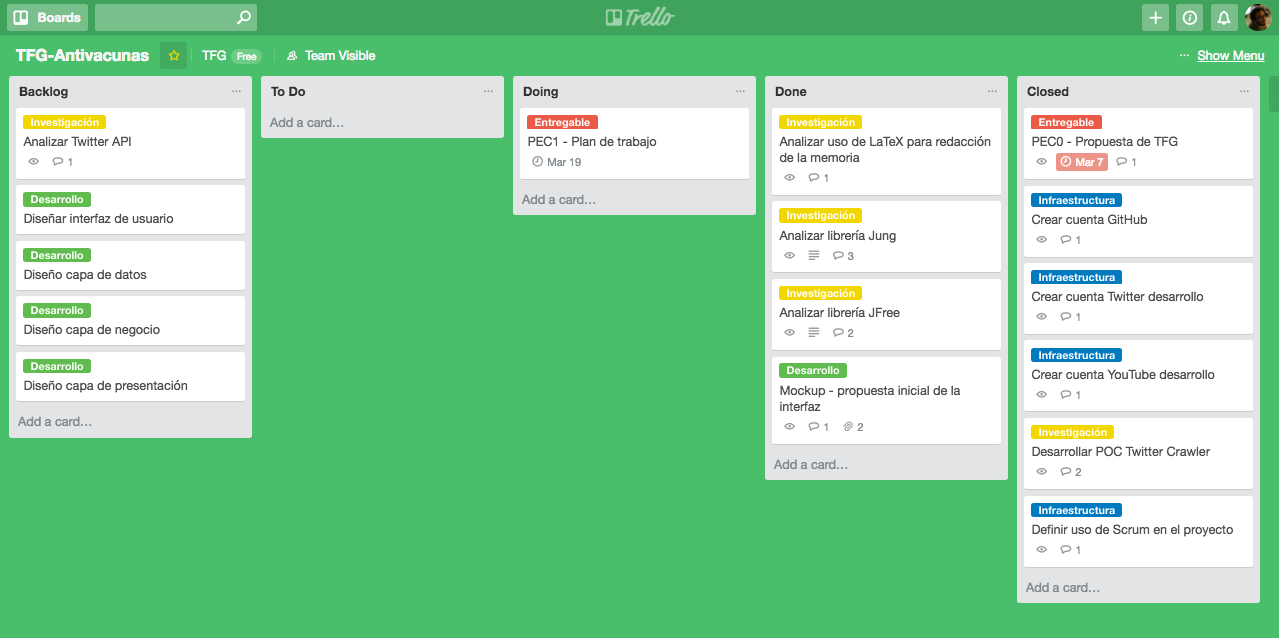
\includegraphics[scale=0.28]{planificacion/trello-backlog.png}
\caption{Ejemplo del backlog del proyecto en Trello}
\end{figure}
\medskip 

\subsection{Planificación del Trabajo}\label{planificacionTrabajao} 
En la realización del proyecto se propuso inicialmente seguir una planificación tentativa tal y como se detalla en el diagrama de \textit{Grantt} facilitado en las figuras dos y tres:

\begin{figure}[H]
\centering
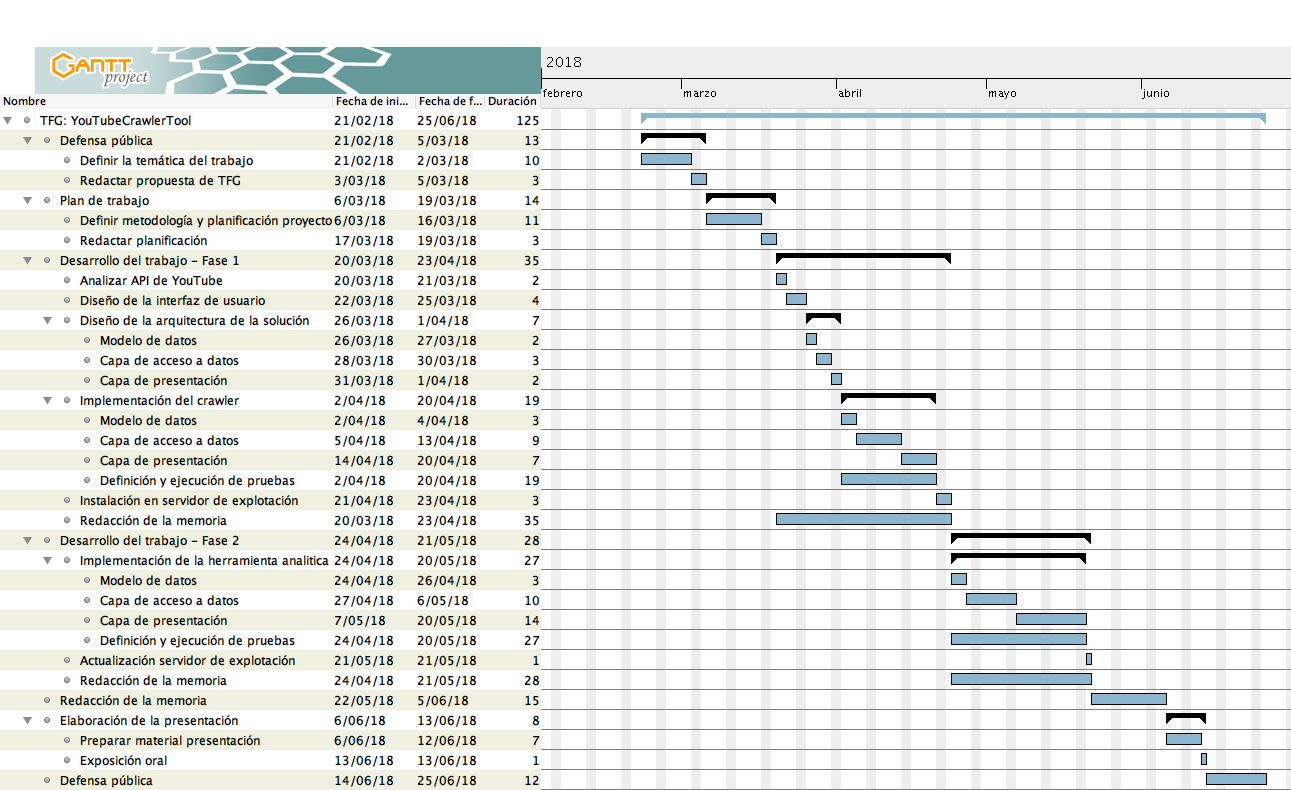
\includegraphics[scale=0.25]{planificacion/planificacion.png}
\caption{Listado de tareas y diagrama de Gantt}
\end{figure}

\begin{figure}[H]
\centering
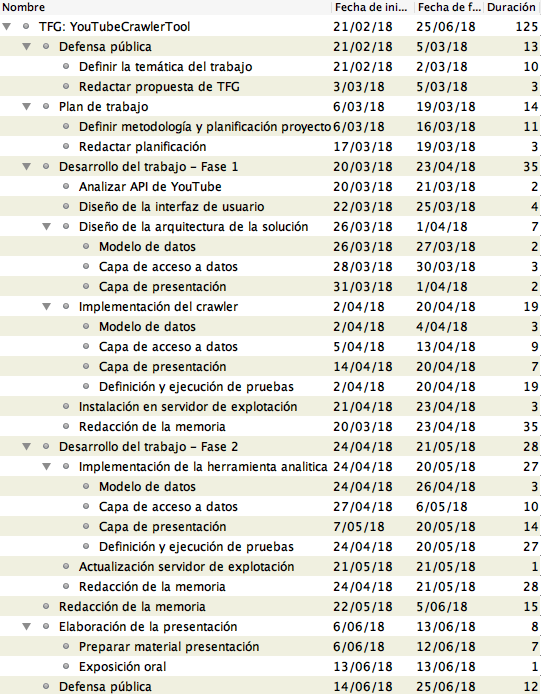
\includegraphics[scale=0.4]{planificacion/listado-tareas.png}
\caption{Listado de tareas}
\end{figure}
\newpage

De la planificación inicial cabe destacar que la redacción de la memoria se diseño como una tarea evolutiva que se desarrollaría durante todas las fases del proyecto pero mas intensamente durante la antepenúltima fase dedicada exclusivamente a su redacción. Además, durante las dos fases de desarrollo se  planificaron dos tareas recurrentes para la definición y realización de pruebas de calidad del producto a realizar durante todo el ciclo de desarrollo.
\\

Como se puede observar, en el diagrama facilitado en cada entrega se pretendían conseguir unos hitos concretos. La relación de los mas destacables por entrega son los siguientes:

\begin{itemize}
\item \textbf{Definición de los contenidos del trabajo:} Redacción propuesta TFG.
\item \textbf{Plan de trabajo:} Redacción planificación.
\item \textbf{Desarrollo del trabajo – Fase 1:} Instalación en servidor de explotación de la primera versión de la aplicación con funcionalidad de \textit{crawler} implementada.
\item \textbf{Desarrollo del trabajo – Fase 2:} Actualización en servidor de explotación de la versión final de la aplicación con funcionalidad analítica implementada.
\item \textbf{Redacción de la memoria:} Entrega de la memoria del proyecto.
\item \textbf{Elaboración de la presentación:} Realizar exposición oral.
\item \textbf{Defensa pública:} Defender públicamente el proyecto.
\end{itemize}

Los riesgos detectados en la planificación inicial se concentraban principalmente en la consecución del hito definido en la primera fase de desarrollo. Para permitir a la clienta de la aplicación poder empezar a recopilar datos para su investigación lo antes posible, se decidió realizar la instalación de la aplicación desarrollada en un entorno de explotación en dos fases distintas, una con la funcionalidad del \textit{crawler} y otra con la funcionalidad analítica implementada. La demora en la primera fase de desarrollo podría comprometer el éxito de la investigación del cliente. Para mitigar este riesgo se realizo el seguimiento del mismo durante las diferentes iteraciones en esa fase de desarrollo. 
\\

Cabe destacar que el diagrama proporcionado en esta sección representa la estimación inicial de la planificación del proyecto de forma tentativa y fue sujeto a modificaciones al inicio de cada nueva fase de desarrollo para garantizar el éxito del proyecto. En la sección de conclusiones del presente documento en el apartado \ref{sec:seguiminetoPlanificacion} se realiza una comparación entre la planificación inicial y sus respectivas revisiones.
\newpage


\subsection{Arquitectura tecnológica}
Para la consecución de los objetivos definidos se ha desarrollado una aplicación web bautizada como \textit{YouTubeCrawlerTool} la cual ha sido diseñada por capas.
\\

En la capa de datos se utiliza una base de datos orientada a grafos \cite{10} la cual nos permite persistir los vídeos obtenidos en forma de grafo junto con sus relaciones ademas de otras informaciones derivadas y necesarias para el uso y funcionamiento de la aplicación.
\\

La capa de aplicación ha sido desarrollada con tecnología Java EE \cite{11} implementada mayormente utilizando proyectos del marco de desarrollo \textit{Spring Framework} \cite{12} entre otros. En esta capa se hace uso intensivo de servicios externos en forma de API pública ofrecida por \textit{YouTube} con el fin de consumir dicha API para recolectar los vídeos requeridos por el usuario para su estudio.
\\

Finalmente, en la capa de cliente las vistas desarrolladas utilizan lenguaje JavaScript \cite{13} con un gran uso de \textit{JQuery} \cite{14} para modificar el DOM y realizar llamadas asíncronas a la API REST habilitada en la capa de aplicación para tales efectos.
\\

En los siguientes apartados se profundiza en la arquitectura y el diseño de la aplicación introducidos en esta sección.
\medskip 

\subsection{Resumen de capítulos}
En los próximos capítulos se detalla el trabajo realizado juntamente con los productos obtenidos y sus conclusiones. La relación de capítulos es la siguiente:

\begin{itemize}
\item \textbf{Análisis y diseño:} Explicación de la metodología de diseño escogida así como los pasos que se llevaron a cabo para definir una propuesta a la clienta y su posterior análisis para acabar definiendo la arquitectura de la solución.
\item \textbf{Desarrollo:} Descripción del desarrollo efectuado y de las decisiones realizadas durante el proceso.
\item \textbf{Implementación y puesta en funcionamiento:} Detalle de los productos obtenidos con las instrucciones para su correcta puesta en funcionamiento ademas de las acciones de formación realizadas.
\item \textbf{Conclusiones:} Sumario de resultados obtenidos y conclusiones sobre el trabajo realizado.
\end{itemize}

\newpage 



\section{Análisis y diseño}
\bigskip 

\subsection{Metodología}\label{metodologia} 
Para realizar el diseño de la aplicación se opto de entre diferentes posibilidades el enfoque definido por la filosofía del 'Diseño centrado en el usuario' \cite{15}.
\\

El diseño centrado en el usuario, como bien indica su nombre, se caracteriza por conocer a fondo a los futuros usuarios de una aplicación para diseñar un producto que resuelva sus necesidades y expectativas buscando en todo momento conseguir la mayor satisfacción del usuario posible. Se trata de un proceso iterativo y cíclico por fases en donde en cada una de ellas se utilizan distintas técnicas para conseguir los objetivos propuestos. 
\\

En nuestro proyecto se ha decidido seguir esta y no otra metodología de diseño tales como el 'Diseño centrado en la actividad' o el 'Diseño centrado en el uso' debido a que, como en nuestro caso la clienta de la aplicación va a ser también la usuaria final de la misma, se ha decidido realizar el análisis de la aplicación centrada en ella y sus necesidades por encima de la actividad que se llevara a cabo o el uso.
\\

La relación de fases y técnicas utilizadas ha sido la siguiente:

\begin{itemize}
\item \textbf{Definir contexto de uso:} El objetivo de esta fase es el de determinar que necesidades pretende la usuaria final que la aplicación resuelva y a que se va a destinar su uso. La técnica escogida para la realización de esta fase fueron las entrevistas con la usuaria final que se realizaron mediante videoconferencia sobretodo durante las diferentes \textit{sprint reviews} al termino de cada \textit{sprint}.
\item \textbf{Especificar requisitos:} En la siguiente fase se definen los requisitos del sistema a partir de la información recogida en la fase previa. Para los requisitos funcionales se opto por recogerlos como 'casos de uso' \cite{16}.
\item \textbf{Diseñar el producto:} En esta fase se diseñan y implementan los requisitos definidos en la fase anterior ya sea con el objetivo de proporcionar una solución final o una propuesta de solución a ser refinada en sucesivas iteraciones. Las técnicas utilizadas en esta fase fueron la creación de maquetas para evaluar la solución y el prototipo mediante pruebas de concepto realizadas con el objetivo de estudiar posibles soluciones antes de realizar su implementación en la aplicación.
\item \textbf{Poner a prueba el producto:} Finalmente, en esta fase se pone a prueba el producto obtenido. Para hacerlo, se definieron y ejecutaron pruebas de integración diseñadas teniendo en cuenta los casos de uso definidos previamente y se realizaron test con usuarios para evaluar su grado de satisfacción.
\end{itemize}

Gracias al enfoque escogido fue posible encontrar respuestas a preguntas sobre las expectativas que la usuaria tenia depositadas sobre la aplicación y que fueron de gran ayuda a la hora de diseñar la solución final. Algunas de las principales preguntas fueron:\\
\textit{¿Quiénes son los usuarios de la aplicación?}\\
\textit{¿Cuáles son las tareas a realizar?}\\
\textit{¿Qué funcionalidades se necesitan?}\\
\textit{¿Qué información se necesita?}
\\

También cabe destacar que gracias a que tanto \textit{Scrum} como el diseño centrado en el usuario son dos procesos iterativos, resulto fácil integrar esta metodología dentro del marco ágil de desarrollo.
\medskip 

\subsection{Propuesta de la solución}
\medskip 

\subsubsection{Reuniones y entrevistas}
Tal y como se ha introducido en la sección \ref{metodologia} sobre la metodología de diseño utilizada, para definir el contexto de uso y conocer las necesidades a ser cubiertas por la aplicación, se realizaron varias entrevistas con la clienta y los \textit{stakeholders} donde la gran mayoría de ellas fueron dentro del contexto de \textit{scrum} como reuniones de \textit{sprint review} y \textit{sprint planning}.
\\

A continuación se resumen las entrevistas y reuniones realizadas junto con los principales temas tratados y decisiones tomadas:
\\

\noindent\textbf{Fecha:} 05/03/2018
\\
\noindent\textbf{Hora de inicio:} 21:00
\\
\noindent\textbf{Hora final:} 21:45
\\
\noindent\textbf{Asistentes:} 
\begin{itemize}
\item Carlos Luis Sánchez Bocanegra: \textit{stakeholder}
\item Johanna Milena Rodríguez Vera: clienta
\item Javier Sánchez Mendoza: \textit{product owner}, \textit{scrum master} y desarrollador
\end{itemize}
\noindent\textbf{Temas tratados:}
\begin{itemize}
\item Que conocimiento sobre el movimiento antivacunas se quiere obtener. 
\item Que se pretende hacer con la información recolectada.
\item Definición de los objetivos de la aplicación.
\end{itemize}
\noindent\textbf{Decisiones:}
\begin{itemize}
\item La clienta definirá los criterios de búsqueda y el conocimiento que debe ser obtenido por la aplicación.
\item El análisis de los datos los realizara la clienta con herramientas especializadas.
\item El objetivo principal de la aplicación es la obtención de datos mediante búsquedas en redes sociales.
\item La aplicación debe ofrecer funcionalidad para exportar los datos recolectados a otras herramientas.
\end{itemize}

\begin{center}\rule{10cm}{0.4pt}\end{center}

\noindent\textbf{Fecha:} 12/03/2018
\\
\noindent\textbf{Hora de inicio:} 21:00
\\
\noindent\textbf{Hora final:} 21:30
\\
\noindent\textbf{Asistentes:} 
\begin{itemize}
\item Carlos Luis Sánchez Bocanegra: \textit{stakeholder}
\item Johanna Milena Rodríguez Vera: clienta
\item Javier Sánchez Mendoza: \textit{product owner}, \textit{scrum master} y desarrollador
\end{itemize}
\noindent\textbf{Temas tratados:}
\begin{itemize}
\item Alcance del estudio a realizar.
\item Sobre que redes sociales debe centrarse el estudio.
\end{itemize}
\noindent\textbf{Decisiones:}
\begin{itemize}
\item Se decide adoptar el marco de trabajo \textit{scrum} para la realización del proyecto.
\item El estudio se centrara inicialmente en una sola red social a determinar.
\item En la aplicación sera posible ejecutar varios procesos de recolección de datos al mismo tiempo.
\item Se incorporara una sección para analizar los datos obtenidos de forma visual (por definir).
\item El \textit{product owner} realizara una propuesta inicial de la interfaz de usuario.
\end{itemize}

\begin{center}\rule{10cm}{0.4pt}\end{center}

\noindent\textbf{Fecha:} 19/03/2018
\\
\noindent\textbf{Hora de inicio:} 21:00
\\
\noindent\textbf{Hora final:} 21:30
\\
\noindent\textbf{Asistentes:} 
\begin{itemize}
\item Carlos Luis Sánchez Bocanegra: \textit{stakeholder}
\item Johanna Milena Rodríguez Vera: clienta
\end{itemize}
\noindent\textbf{Temas tratados:}
\begin{itemize}
\item Comentarios sobre la propuesta inicial de la interfaz de usuario realizada por el \textit{product owner}.
\item Pros y contras sobre la elección de \textit{Twitter} como red social para el estudio.
\end{itemize}
\noindent\textbf{Decisiones:}
\begin{itemize}
\item Elección de \textit{Twitter} como red social a utilizar en el estudio.
\item La aplicación incluirá una visualización en forma de grafo para poder analizar visualmente las relaciones existente en la información recolectada y descubrir patrones.
\item El \textit{product owner} debe estudiar la viabilidad de utilizar \textit{Twitter} para la consecución de los objetivos. 
\end{itemize}

\begin{center}\rule{10cm}{0.4pt}\end{center}

\noindent\textbf{Fecha:} 26/03/2018
\\
\noindent\textbf{Hora de inicio:} 21:00
\\
\noindent\textbf{Hora final:} 21:45
\\
\noindent\textbf{Asistentes:} 
\begin{itemize}
\item Carlos Luis Sánchez Bocanegra: \textit{stakeholder}
\item Johanna Milena Rodríguez Vera: clienta
\end{itemize}
\noindent\textbf{Temas tratados:}
\begin{itemize}
\item Debido a las limitaciones de uso detectadas en la API de \textit{Twitter}, se propone utilizar la red social \textit{YouTube} como alternativa.
\item Definición del grafo a utilizar y que elementos actuaran como nodo y aristas.  
\end{itemize}
\noindent\textbf{Decisiones:}
\begin{itemize}
\item Elección de \textit{YouTube} como red social a utilizar en el estudio.
\item El \textit{product owner} debe estudiar la viabilidad de utilizar \textit{YouTube} para la consecución de los objetivos. 
\item Actualizar la propuesta de interfaz de usuario para reflejar el cambio de red social.
\end{itemize}

\begin{center}\rule{10cm}{0.4pt}\end{center}

\noindent\textbf{Fecha:} 05/04/2018
\\
\noindent\textbf{Hora de inicio:} 21:00
\\
\noindent\textbf{Hora final:} 21:45
\\
\noindent\textbf{Asistentes:} 
\begin{itemize}
\item Carlos Luis Sánchez Bocanegra: \textit{stakeholder}
\item Johanna Milena Rodríguez Vera: clienta
\item Javier Sánchez Mendoza: \textit{product owner}, \textit{scrum master} y desarrollador
\end{itemize}
\noindent\textbf{Temas tratados:}
\begin{itemize}
\item Comentarios sobre la propuesta inicial de la interfaz de usuario realizada por el \textit{product owner}.
\item Analizar criterios de búsqueda y información devuelta por la API de \textit{YouTube}
\item Detección de vídeos duplicados.
\item Detectar usuarios \textit{influencers} a partir de la información obtenida.
\item Avances en la definición de los componentes del grafo.
\end{itemize}
\noindent\textbf{Decisiones:}
\begin{itemize}
\item Criterios de búsqueda de \textit{YouTube} a utilizar para recolectar los vídeos.
\item Campos a almacenar de cada vídeo.
\item Incorporar funcionalidad para ver resumen de las búsquedas realizadas junto con la información recolectada con pre visualización de vídeos.
\item Utilizar una variable pre calculada (bautizada como "\textit{scopeRange}") para determinar el tamaño de los nodos al ser visualizados en el grafo.
\end{itemize}

\begin{center}\rule{10cm}{0.4pt}\end{center}

\noindent\textbf{Fecha:} 12/04/2018
\\
\noindent\textbf{Hora de inicio:} 21:30
\\
\noindent\textbf{Hora final:} 22:15
\\
\noindent\textbf{Asistentes:} 
\begin{itemize}
\item Carlos Luis Sánchez Bocanegra: \textit{stakeholder}
\item Johanna Milena Rodríguez Vera: clienta
\item Javier Sánchez Mendoza: \textit{product owner}, \textit{scrum master} y desarrollador
\end{itemize}
\noindent\textbf{Temas tratados:}
\begin{itemize}
\item Comentarios sobre la visualización en grafo.
\item Identificación de vídeos pro y anti vacunación.
\end{itemize}
\noindent\textbf{Decisiones:}
\begin{itemize}
\item Queda definida la visualización en grafo.
\item Los contenidos a visualizar en el grafo podrán ser filtrados.
\item Se define funcionalidad para etiquetar los vídeos recolectados utilizando categorías previamente definidas por el usuario en la aplicación.
\item En la aplicación habrá dos tipos de usuarios, usuarios anónimos que no podrán realizar acciones de escritura ni borrado y usuarios registrados que podrán realizar todas la acciones.
\item Incorporar visualizaciones estadísticas sobre el uso de las categorías.
\item Realización de una ultima propuesta de interfaz de usuario que recoja los últimos cambios propuestos junto con la visualización en grafo.
\end{itemize}

\begin{center}\rule{10cm}{0.4pt}\end{center}

\noindent\textbf{Fecha:} 19/04/2018
\\
\noindent\textbf{Hora de inicio:} 21:30
\\
\noindent\textbf{Hora final:} 22:00
\\
\noindent\textbf{Asistentes:} 
\begin{itemize}
\item Carlos Luis Sánchez Bocanegra: \textit{stakeholder}
\item Johanna Milena Rodríguez Vera: clienta
\item Javier Sánchez Mendoza: \textit{product owner}, \textit{scrum master} y desarrollador
\end{itemize}
\noindent\textbf{Temas tratados:}
\begin{itemize}
\item Comentarios sobre la propuesta de interfaz de usuario. 
\item Priorización de funcionalidades.
\end{itemize}
\noindent\textbf{Decisiones:}
\begin{itemize}
\item La clienta da por aprobada la propuesta de interfaz de usuario.
\item Definición de valores por defecto al realizar las búsquedas de contenidos.
\item Las funcionalidades estadísticas y de visualización de canales quedan asignadas con una prioridad secundaria en relación a otras funcionalidades.
\item Se va a buscar la colaboración de un estadista para definir la formula de la variable "\textit{scopeRange}".
\end{itemize}

\begin{center}\rule{10cm}{0.4pt}\end{center}

\noindent\textbf{Fecha:} 26/04/2018
\\
\noindent\textbf{Hora de inicio:} 21:00
\\
\noindent\textbf{Hora final:} 21:30
\\
\noindent\textbf{Asistentes:} 
\begin{itemize}
\item Carlos Luis Sánchez Bocanegra: \textit{stakeholder}
\item Johanna Milena Rodríguez Vera: clienta
\item Javier Sánchez Mendoza: \textit{product owner}, \textit{scrum master} y desarrollador
\end{itemize}
\noindent\textbf{Temas tratados:}
\begin{itemize}
\item Seguimiento de la implementación de la aplicación
\item Seguimiento de la definición de la fórmula para calcular el alcance de los vídeos ("\textit{scopeRange}").
\end{itemize}
\noindent\textbf{Decisiones:}

\begin{center}\rule{10cm}{0.4pt}\end{center}

\noindent\textbf{Fecha:} 03/05/2018
\\
\noindent\textbf{Hora de inicio:} 21:00
\\
\noindent\textbf{Hora final:} 21:30
\\
\noindent\textbf{Asistentes:} 
\begin{itemize}
\item Carlos Luis Sánchez Bocanegra: \textit{stakeholder}
\item Johanna Milena Rodríguez Vera: clienta
\item Javier Sánchez Mendoza: \textit{product owner}, \textit{scrum master} y desarrollador
\end{itemize}
\noindent\textbf{Temas tratados:}
\begin{itemize}
\item Seguimiento de la implementación de la aplicación.
\item Seguimiento de la definición de la fórmula para calcular el alcance de los vídeos ("\textit{scopeRange}").
\end{itemize}
\noindent\textbf{Decisiones:}

\begin{center}\rule{10cm}{0.4pt}\end{center}

\noindent\textbf{Fecha:} 10/05/2018
\\
\noindent\textbf{Hora de inicio:} 20:30
\\
\noindent\textbf{Hora final:} 21:00
\\
\noindent\textbf{Asistentes:} 
\begin{itemize}
\item Carlos Luis Sánchez Bocanegra: \textit{stakeholder}
\item Johanna Milena Rodríguez Vera: clienta
\item Javier Sánchez Mendoza: \textit{product owner}, \textit{scrum master} y desarrollador
\end{itemize}
\noindent\textbf{Temas tratados:}
\begin{itemize}
\item Seguimiento de la implementación de la aplicación.
\item Seguimiento de la definición de la fórmula para calcular el alcance de los vídeos ("\textit{scopeRange}").
\end{itemize}
\noindent\textbf{Decisiones:}
\begin{itemize}
\item Instalación de la aplicación en entorno de explotación durante la próxima semana.
\item Mientras no se disponga de la formula para la variable "\textit{scopeRange}", utilizar formula alternativa definida por la clienta.
\end{itemize}

\begin{center}\rule{10cm}{0.4pt}\end{center}

\noindent\textbf{Fecha:} 17/05/2018
\\
\noindent\textbf{Hora de inicio:} 20:30
\\
\noindent\textbf{Hora final:} 21:30
\\
\noindent\textbf{Asistentes:} 
\begin{itemize}
\item Carlos Luis Sánchez Bocanegra: \textit{stakeholder}
\item Johanna Milena Rodríguez Vera: clienta
\item Javier Sánchez Mendoza: \textit{product owner}, \textit{scrum master} y desarrollador
\end{itemize}
\noindent\textbf{Temas tratados:}
\begin{itemize}
\item Presentación de la aplicación desarrollada y formación a la clienta.
\end{itemize}
\noindent\textbf{Decisiones:}
\begin{itemize}
\item Se decide utilizar la formula alternativa propuesta por la clienta para la variable "\textit{scopeRange}".
\item Añadir nueva funcionalidad de favoritos.
\item Realización de cambios en la visualización de los listados de los vídeos.
\end{itemize}

\begin{center}\rule{10cm}{0.4pt}\end{center}

En los siguientes apartados se detallan algunas de las decisiones tomadas en estas reuniones las cuales tuvieron mas repercusión en el resultado final de la aplicación.
\medskip 

\subsubsection{Elección de YouTube como red social}\label{eleccionYouTube} 
A la hora de escoger una red social para realizar el estudio del movimiento antivacuna nos encontramos con una gran variedad de opciones, tales como \textit{Facebook}, \textit{Twitter} o \textit{YouTube} para nombrar solo algunas.
\\

Johanna, clienta de la aplicación y la encargada de realizar el estudio, mostró su predilección inicial por \textit{Twitter}. En su criterio, \textit{Twitter} presentaba una estructuración de la información que favorecía su posterior análisis y estudio al basarse, principalmente, un mensaje (\textit{tweet}) de los campos titulo y descripción, hecho que facilitaba la categorización de los contenidos obtenidos. Por otro lado, el uso extensivo de etiquetas en esta red social (\textit{hashtags}) simplificaría el proceso de búsqueda de contenidos. Por lo referente al alcance de la red social, Johanna consideraba que a nivel de usuarios y actividad relacionada con la vacunación, \textit{Twitter} superaba a otras redes sociales tales como \textit{YouTube}.
\\

Debido a estas consideraciones, \textit{Twitter} fue escogida inicialmente como la red social a utilizar en el proyecto. Por este motivo, inicialmente la aplicación desarrollada se llamaba \textit{TwitterCrawlerTool} y las primeras versiones de la propuesta de interfaz de usuario se habían realizado teniendo en consideración a \textit{Twitter} como red social escogida. Incluso, una prueva de concepto llego a desarrollarse: \href{https://github.com/jsanchezmend/TFGAntivacunas/tree/master/POCTwitterCrawler}{POCTwitterCrawler}.
\\

Con la elección realizada y teniendo desarrollada una prueba de concepto, se procedió al estudio en profundidad de la API de \textit{Twitter} y fue entonces cuando se descubrieron limitaciones sobre su uso. Concretamente, \textit{Twitter} define tres niveles de uso: \textit{Standard}, \textit{Premium} y \textit{Enterprise}; de todas ellas solo la opción \textit{Standard} es completamente gratuita pero, en este caso, con unas severas restricciones de uso a la hora de buscar mensajes \cite{17}. Algunas de las restricciones son:
\begin{itemize}
\item Máximo de 100 \textit{"tweets"} por búsqueda.
\item Información disponible solo de los últimos 7 días.
\item Solo permite búsqueda textual, no se permite búsqueda temporal.
\end{itemize}

A causa de estas restricciones, resultaba imposible poder recabar información con una antigüedad inferior a siete días o realizar comparaciones en el tiempo sobre la evolución de los movimientos pro y anti vacunas, hecho que es requerido en el estudio. Ante los descubrimientos realizados se decidió explorar otras alternativas al uso de \textit{Twitter}.
\\

Fue entonces que la opción de utilizar \textit{YouTube} como red social de estudio en el proyecto se considero en profundidad. Y es que aunque se llegara anteriormente a la conclusión de que \textit{Twitter} tenia un alcance mayor en numero de usuarios y potencial de contenidos a obtener, no se debe desestimar tampoco el alcance de \textit{YouTube} que, si bien inicialmente no era considerada como una red social al uso, a día de hoy el numero de usuarios que no solo visualizan sus vídeos sino que también comparten contenidos y comentarios crece día a día, convirtiendo a \textit{YouTube} como una buena opción para encontrar la información requerida. Y en lo referente a la estructuración de la información, debido a que juntamente con los vídeos se provee un titulo y una descripción no era necesario cambiar el enfoque dado inicialmente en este sentido.
\\

Por lo referente a la API ofrecida por \textit{YouTube} para la obtención de contenidos, los criterios de búsqueda disponibles son mucho mas amplios que los ofrecidos por \textit{Twitter}, permitiéndonos entre otras posibilidades, filtrar los contenidos a obtener por rangos de fechas. No existe limitación a la hora de obtener contenidos independientemente de su fecha de publicación (en todo caso posterior a 14/02/2005, fecha de fundación de \textit{YouTube}). Y en relación a limitaciones en el volumen de información a obtener, \textit{YouTube} no impone limitaciones por búsqueda, lo que posibilita obtener toda la información requerida sobre un termino en concreto. En su defecto, \textit{YouTube} utiliza un sistema de cuotas que se aplica a periodos de tiempo en concreto \cite{18}, por ejemplo, en su versión gratuita permite realizar hasta 1.000.000 de operaciones de lectura por día que, tal y como se ha demostrado, han sido suficientes para el uso dado a la aplicación desarrollada. Para estudiar su viabilidad en el proyecto, se realizo una prueba de concepto con resultados satisfactorios: \href{https://github.com/jsanchezmend/TFGAntivacunas/tree/master/POCYouTubeCrawler}{POCYouTubeCrawler}.
\\

En el apartado \ref{youTubeDataAPI} se detalla en profundidad los servicios de la API de \textit{YouTube} utilizados y el modo en que la aplicación los consume para obtener contenidos. 
\medskip 

\subsubsection{Visualización de vídeos en grafo}\label{propuestaGrafo} 
Otra de las decisiones de diseño mas debatidas fue la definición de una vista en la aplicación que permitiera de forma visual analizar como se relacionan los movimientos anti y pro vacuna en la red social de \textit{YouTube}. 
\\

La motivación principal de la misma es la de proporcionar una funcionalidad con la cual fuera posible estudiar las vías de acceso a los contenidos y observar que movimiento tiene mas alcance de audiencia en \textit{YouTube}. Para tales efectos, se llego a la conclusión que una visualización en formato de grafo donde fuera posible distinguir los dos movimientos a estudio seria la forma mas efectiva de representar dicha información.
\\

Para difinir el grafo, necesitábamos analizar que componentes actuarían como nodo y que representarían las aristas entre ellos, ademas de tomar otras decisiones como si se incorporarían pesos al grafo y si este seria dirigido o no. Para ayudar en la definición del grafo, se realizaron propuestas que se apoyaron con pruebas realizadas manualmente por parte de la clienta con contenidos reales:

\begin{figure}[H]
\centering
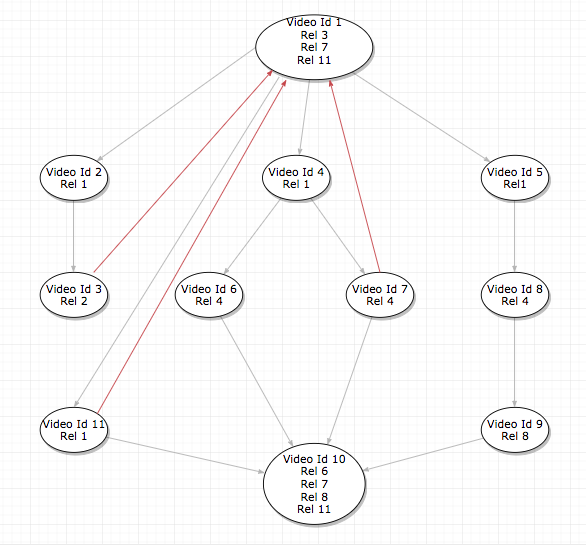
\includegraphics[scale=0.40]{grafo/propuesta1.png}
\caption{Propuesta grafo dirigido}
\end{figure}

\begin{figure}[H]
\centering
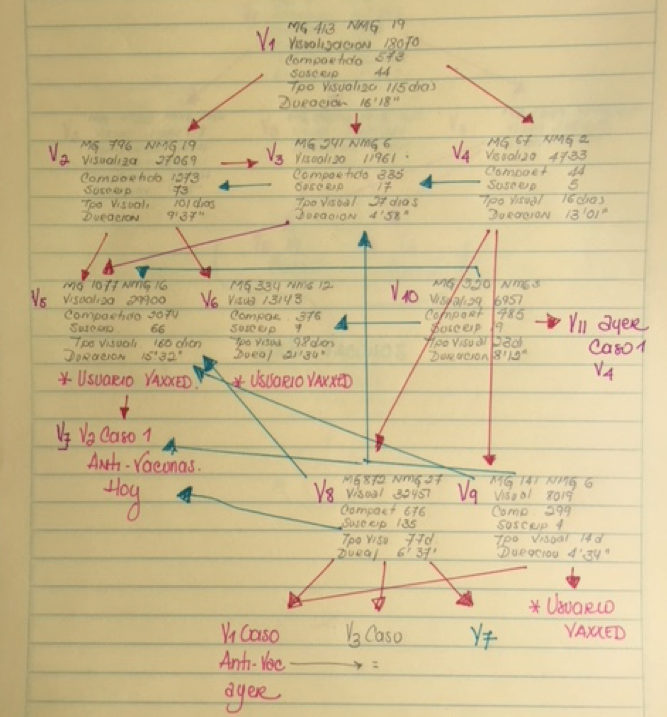
\includegraphics[scale=0.40]{grafo/pruebaManual.png}
\caption{Maqueta de grafo dirigido}
\end{figure}
\bigskip 

Como conclusiones del análisis realizado se definió el grafo a representar con las siguientes características:
\begin{itemize}
\item \textbf{Tipo:} Grafo dirigido sin pesos.
\item \textbf{Nodos:} Vídeos y canales (canales de forma opcional).
\item \textbf{Aristas:} Entre dos vídeos representa que desde el vídeo origen es posible acceder al vídeo destino (mediante la recomendación realizada por \textit{YouTube} como vídeos relacionados). Y entre un vídeo y un canal representa que el vídeo (nodo origen) ha sido publicado por el canal relacionado (nodo destino).
\item \textbf{Visualización:} En nodos tipo vídeo, su tamaño sera determinado por su alcance de audiencia y el color de representación sera determinado por su categoría (anti o pro vacuna). En el caso de nodos tipo canal su tamaño y representación no sera determinado por ninguna de sus características, por lo que todos los canales se visualizaran con el mismo formato pero diferenciados de los nodos tipo vídeo. Sera posible ver una pre visualización del contenido al hacer clic en el.
\end{itemize}

Para estudiar su viabilidad, se realizo una prueba de concepto con resultado favorable: \href{https://github.com/jsanchezmend/TFGAntivacunas/tree/master/POCYouTubeCrawler}{POCYouTubeCrawler}.
\begin{figure}[H]
\centering
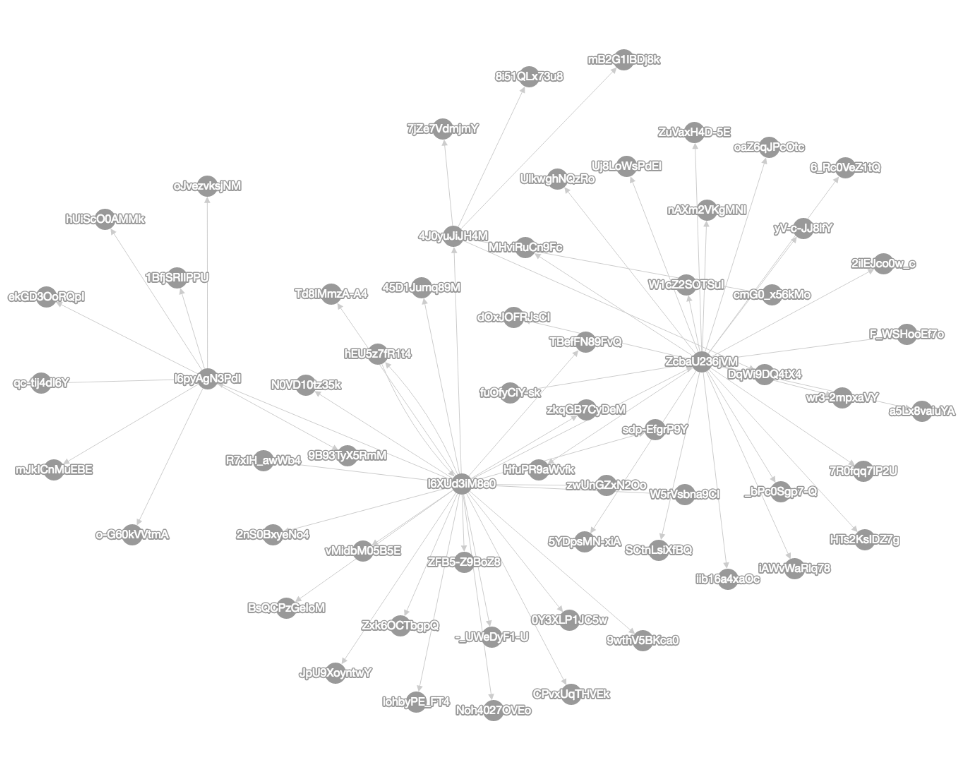
\includegraphics[scale=0.30]{grafo/pocGrafo.png}
\caption{Prueba de concepto de grafo dirigido}
\end{figure}

En la propuesta de grafo detallada, se detectaron dos requerimientos encubiertos necesarios para su realización: la necesidad de categorizar vídeos y la definición de una variable que nos permitiera determinar el alcance de audiencia de un vídeo para definir su tamaño en el grafo.
\\

Para la categorización de los vídeos, se diseño una funcionalidad genérica que permitiera al usuario definir las categorías necesarias con las cuales posteriormente poder etiquetar los vídeos. El inconveniente de esta solución es que para poder visualizar correctamente el grafo y identificar los grupos de nodos, se requiere realizar previamente una tarea de categorización manual de los vídeos. Después de analizar la problemática, debido a que el volumen de datos requeridos para realizar el estudio se determino en una cifra menor a mil, se acepto la solución como viable pero, en este caso, se debía tener presente esta circunstancia en la planificación del proyecto.
\\

Por otro lado, para definir el tamaño de visualización del nodo se estudio la creación de una variable apodada como \textit{scopeRange}. Dicha variable, debía representar dentro de un rango de valores valido, el alcance o popularidad obtenido por un vídeo en concreto. Para ello se estudio poder identificar a los usuarios mas influyentes de \textit{YouTube} (conocidos como \textit{influencers}), pero finalmente se decidió utilizar la información estadística ofrecida por \textit{YouTube} para cada vídeo, la cual se compone de los campos:
\begin{itemize}
\item \textbf{\textit{viewCount}:} Numero de visualizaciones del vídeo.
\item \textbf{\textit{likeCount}:} Numero de personas a las cuales le ha gustado el vídeo.
\item \textbf{\textit{dislikeCount}:} Numero de personas a las cuales no le ha gustado el vídeo.
\item \textbf{\textit{commentCount}:} Numero de comentario que ha recibido el vídeo.
\end{itemize}

Para la definición de la formula se pidió la colaboración de un estadista. Pero debido a que la fecha final de desarrollo del proyecto se aproximaba y aun no se disponía de la colaboración, se opto por aplicar una formula definida por la clienta que en las pruebas realizadas demostró efectividad:
\begin{center}
$$scopeRange = \frac{likeCount}{dislikeCount}$$
\end{center}
Con un valor mínimo definido de 10 para asegurar la visualización del vídeo en el grafo.
\\

A modo ilustrativo, a continuación se adjunta una imagen de la implementación del grafo en la aplicación:
\begin{figure}[H]
\centering
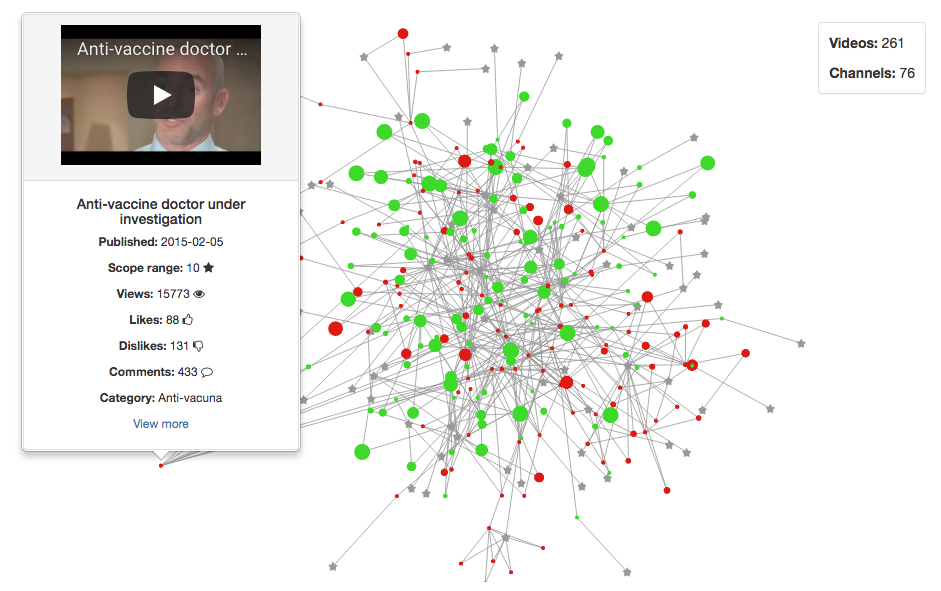
\includegraphics[scale=0.40]{grafo/final.png}
\caption{Implementación del grafo en la aplicación}
\end{figure}
\medskip 

\subsubsection{Casos de uso}\label{casosDeUso} 
Hacer uso de un marco ágil de desarrollo no debe ser escusa para no disponer de una documentación adecuada de los requisitos de una aplicación y, aunque estos sufran modificaciones durante las diferentes iteraciones de desarrollo, estos deben de estar actualizados. Por esta razón se ha decidido realizar la toma de requerimientos de la aplicación en forma de casos de uso, en donde para facilitar la gestión de cambios se ha decidido hacer constar solo el titulo, actores y descripción en cada uno de ellos.
\\

Así entonces y con lo expuesto en apartados anteriores, a continuación se expone una imagen representativa de los casos de uso identificados agrupados por componentes según la funcionalidad realizada y a continuación el listado completo de cada uno de ellos:

\begin{figure}[H]
\centering
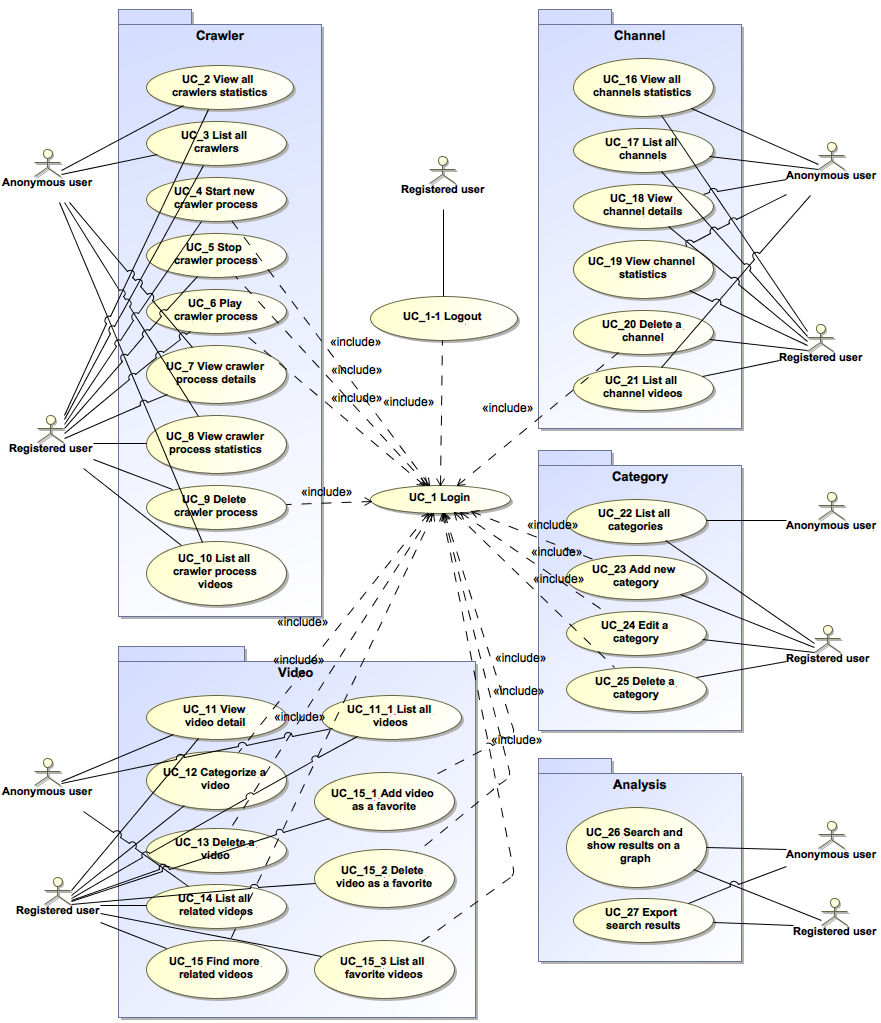
\includegraphics[scale=0.35]{requisitos/UseCases.png}
\caption{Casos de uso}
\end{figure}
\medskip 
\medskip 

\noindent\textbf{Componente \textit{User session}:}
\\

\noindent\textbf{UC\_1: Login}\\
\textbf{Actores:} Usuario anónimo\\
\textbf{Descripción:} Como usuario anónimo, quiero identificarme en la aplicación mediante nombre de usuario y contraseña.
\\

\noindent\textbf{UC\_1-1: logout}\\
\textbf{Actores:} Usuario registrado\\
\textbf{Descripción:} Como usuario identificado, quiero cerrar la sesión actual en la aplicación.
\\

\begin{center}\rule{10cm}{0.4pt}\end{center}

\noindent\textbf{Componente \textit{Crawler}:}
\\

\noindent\textbf{UC\_2: View all crawlers statistics}\\
\textbf{Actores:} Usuario anónimo, Usuario registrado\\
\textbf{Descripción:} Como usuario, quiero ver el total de vídeos recolectados, el porcentaje de categorizados y la distribución de las categorías.
\\

\noindent\textbf{UC\_3: List all crawlers}\\
\textbf{Actores:} Usuario anónimo, Usuario registrado\\
\textbf{Descripción:} Como usuario, quiero ver todos los procesos de recolección que se han iniciado en el sistema.
\\

\noindent\textbf{UC\_4: Start new crawler process}\\
\textbf{Actores:} Usuario registrado\\
\textbf{Descripción:} Como usuario identificado, quiero iniciar un nuevo proceso de recolección de vídeos según criterio de búsqueda introducido.
\\

\noindent\textbf{UC\_5: Stop crawler process}\\
\textbf{Actores:} Usuario registrado\\
\textbf{Descripción:} Como usuario identificado, quiero parar un proceso de recolección de vídeos que este en ejecución.
\\

\noindent\textbf{UC\_6: Play crawler process}\\
\textbf{Actores:} Usuario registrado\\
\textbf{Descripción:} Como usuario identificado, quiero poner en marcha un proceso de recolección previamente detenido.
\\

\noindent\textbf{UC\_7: View crawler process details}\\
\textbf{Actores:} Usuario anónimo, Usuario registrado\\
\textbf{Descripción:} Como usuario, quiero ver el detalle de un proceso de recolección.
\\

\noindent\textbf{UC\_8: View crawler process statistics}\\
\textbf{Actores:} Usuario anónimo, Usuario registrado\\
\textbf{Descripción:} Como usuario, dado un proceso de recolección en concreto quiero ver su total de vídeos recolectados, su porcentaje de categorizados y su distribución de las categorías.
\\

\noindent\textbf{UC\_9: Delete crawler process}\\
\textbf{Actores:} Usuario registrado\\
\textbf{Descripción:} Como usuario identificado, quiero borrar un proceso de recolección en concreto y todos sus vídeos relacionados.
\\

\noindent\textbf{UC\_10: List all crawler process videos}\\
\textbf{Actores:} Usuario anónimo, Usuario registrado\\
\textbf{Descripción:} Como usuario, quiero ver el listado completo de vídeos recolectados por un proceso de recolección en concreto.
\\

\begin{center}\rule{10cm}{0.4pt}\end{center}

\noindent\textbf{Componente \textit{Video}:}
\\

\noindent\textbf{UC\_11-1: List all videos}\\
\textbf{Actores:} Usuario anónimo, Usuario registrado\\
\textbf{Descripción:} Como usuario, quiero ver listados todos los vídeos del sistema.
\\

\noindent\textbf{UC\_11: View video detail}\\
\textbf{Actores:} Usuario anónimo, Usuario registrado\\
\textbf{Descripción:} Como usuario, quiero ver el detalle de un vídeo en concreto.
\\

\noindent\textbf{UC\_12: Categorize a video}\\
\textbf{Actores:} Usuario registrado\\
\textbf{Descripción:} Como usuario identificado, quiero cambiar la categoría asociada a un vídeo en concreto.
\\

\noindent\textbf{UC\_13: Delete a video}\\
\textbf{Actores:} Usuario registrado\\
\textbf{Descripción:} Como usuario identificado, quiero borrar un vídeo en concreto.
\\

\noindent\textbf{UC\_14: List all related videos}\\
\textbf{Actores:} Usuario anónimo, Usuario registrado\\
\textbf{Descripción:} Como usuario, quiero ver listados todos los vídeos relacionados con un  en concreto.
\\

\noindent\textbf{UC\_15: Find more related videos}\\
\textbf{Actores:} Usuario registrado\\
\textbf{Descripción:} Como usuario identificado, quiero iniciar un nuevo proceso de recolección de vídeos para que encuentre vídeos relacionados a un vídeo en concreto.
\\

\noindent\textbf{UC\_15-1: Add a video as a favorite}\\
\textbf{Actores:} Usuario registrado\\
\textbf{Descripción:} Como usuario identificado, quiero añadir un vídeo en concreto al listado de favoritos.
\\

\noindent\textbf{UC\_15-2: Delete a video as a favorite}\\
\textbf{Actores:} Usuario registrado\\
\textbf{Descripción:} Como usuario identificado, quiero eliminar un vídeo en concreto del listado de favoritos.
\\

\noindent\textbf{UC\_15-3: List all favorite videos}\\
\textbf{Actores:} Usuario registrado\\
\textbf{Descripción:} Como usuario identificado, quiero ver el listado de vídeos favoritos.
\\

\begin{center}\rule{10cm}{0.4pt}\end{center}

\noindent\textbf{Componente \textit{Channel}:}
\\

\noindent\textbf{UC\_16: View all channels statistics}\\
\textbf{Actores:} Usuario anónimo, Usuario registrado\\
\textbf{Descripción:} Como usuario, quiero ver el total de canales importados en el sistema.
\\

\noindent\textbf{UC\_17: List all channels}\\
\textbf{Actores:} Usuario anónimo, Usuario registrado\\
\textbf{Descripción:} Como usuario, quiero ver listados todos los canales importado en el sistema.
\\

\noindent\textbf{UC\_18: View channel details}\\
\textbf{Actores:} Usuario anónimo, Usuario registrado\\
\textbf{Descripción:} Como usuario, quiero ver el detalle de un canal en concreto.
\\

\noindent\textbf{UC\_19: View channel statistics}\\
\textbf{Actores:} Usuario anónimo, Usuario registrado\\
\textbf{Descripción:} Como usuario, dado un canal en concreto quiero ver su total de vídeos recolectados, su porcentaje de categorizados y su distribución de las categorías.
\\

\noindent\textbf{UC\_20: Delete a channel}\\
\textbf{Actores:} Usuario registrado\\
\textbf{Descripción:} Como usuario identificado, quiero eliminar un canal en concreto y todos sus vídeos relacionados.
\\

\noindent\textbf{UC\_21: List all channel videos}\\
\textbf{Actores:} Usuario anónimo, Usuario registrado\\
\textbf{Descripción:} Como usuario, dado un canal en concreto quiero ver listados todos sus vídeos relacionados.
\\

\begin{center}\rule{10cm}{0.4pt}\end{center}

\noindent\textbf{Componente \textit{Category}:}
\\

\noindent\textbf{UC\_22: List all categories}\\
\textbf{Actores:} Usuario anónimo, Usuario registrado\\
\textbf{Descripción:} Como usuario, quiero ver todas las categorías dadas de alta en el sistema.
\\

\noindent\textbf{UC\_23: Add new category}\\
\textbf{Actores:} Usuario registrado\\
\textbf{Descripción:} Como usuario identificado, quiero dar de alta una nueva categoría en el sistema definiendo su nombre y color.
\\

\noindent\textbf{UC\_24: Edit a category}\\
\textbf{Actores:} Usuario registrado\\
\textbf{Descripción:} Como usuario identificado, quiero editar el color de una categoría en concreto.
\\

\noindent\textbf{UC\_25: Delete a category}\\
\textbf{Actores:} Usuario registrado\\
\textbf{Descripción:} Como usuario identificado, quiero eliminar una categoría en concreto del sistema y eliminar todos sus vídeos relacionados.
\\

\begin{center}\rule{10cm}{0.4pt}\end{center}

\noindent\textbf{Componente \textit{Analysis}:}
\\

\noindent\textbf{UC\_26: Search and show results on a graph}\\
\textbf{Actores:} Usuario anónimo, Usuario registrado\\
\textbf{Descripción:} Como usuario, quiero realizar una búsqueda de vídeos en el sistema y visualizarlos en un grafo donde los nodos representen los vídeos encontrados y las aristas sus vídeos relacionados.
\\

\noindent\textbf{UC\_27: Export search results}\\
\textbf{Actores:} Usuario anónimo, Usuario registrado\\
\textbf{Descripción:} Como usuario, quiero realizar una búsqueda de vídeos en el sistema y exportarlos a fichero con formato \textit{csv}.
\\


\subsubsection{Propuesta de interfaz de usuario}\label{propuestaInterfazUsuario} 
Finalmente, en la ultima etapa en lo que ha diseño del producto se refiere, se presentaron a la clienta diferentes propuestas de interfaz de usuario que se fueron refinando a medida que se modificaban o definían nuevas funcionalidades. En concreto se presentaron tres propuestas:
\\

\noindent\textbf{Propuesta inicial presentada el 15/03/2018:}

\begin{figure}[H]
\centering
\subfigure[\textit{Twitter} búsqueda]{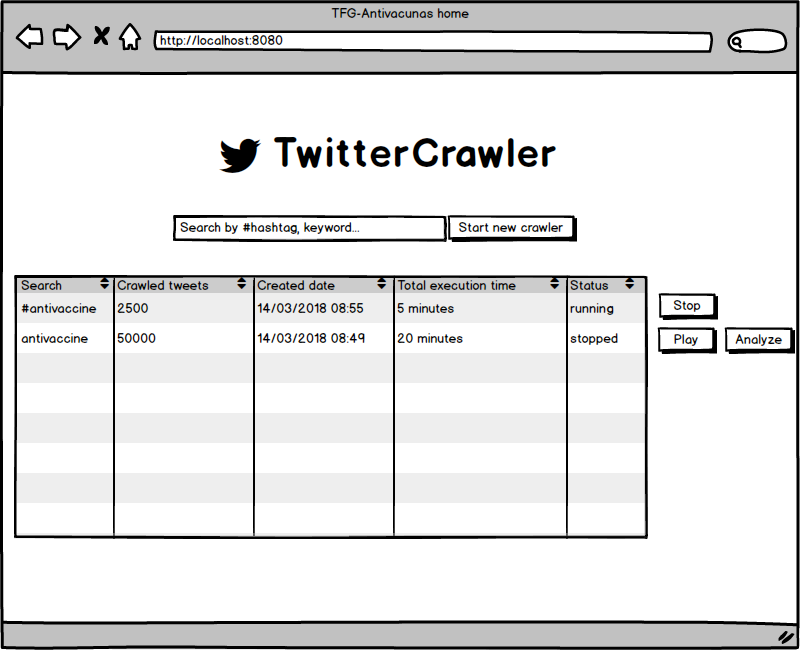
\includegraphics[width=60mm]{interfaz/03-15/1.png}}
\subfigure[\textit{Twitter} análisis]{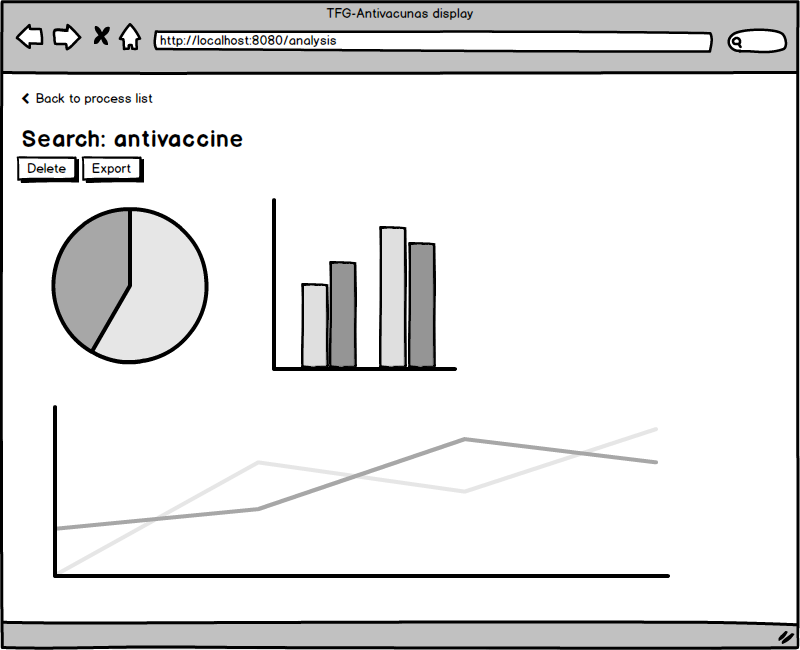
\includegraphics[width=60mm]{interfaz/03-15/2.png}}
\caption{Propuesta inicial interfaz de usuario}
\end{figure}
\pagebreak 

\noindent\textbf{Segunda propuesta presentada el 05/04/2018:}

\begin{figure}[H]
\centering
\subfigure[\textit{YouTube} búsqueda textual]{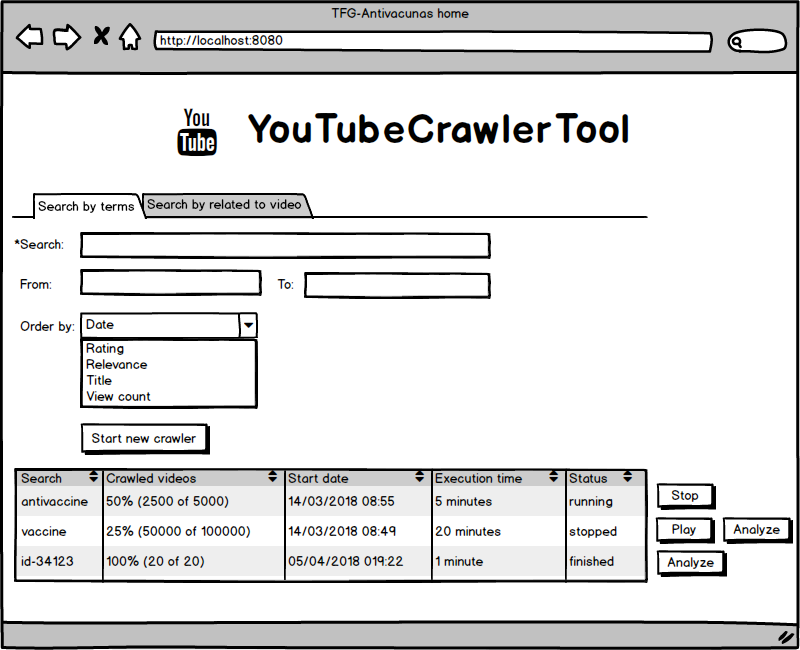
\includegraphics[width=60mm]{interfaz/04-05/1.png}}
\subfigure[\textit{YouTube} análisis textual]{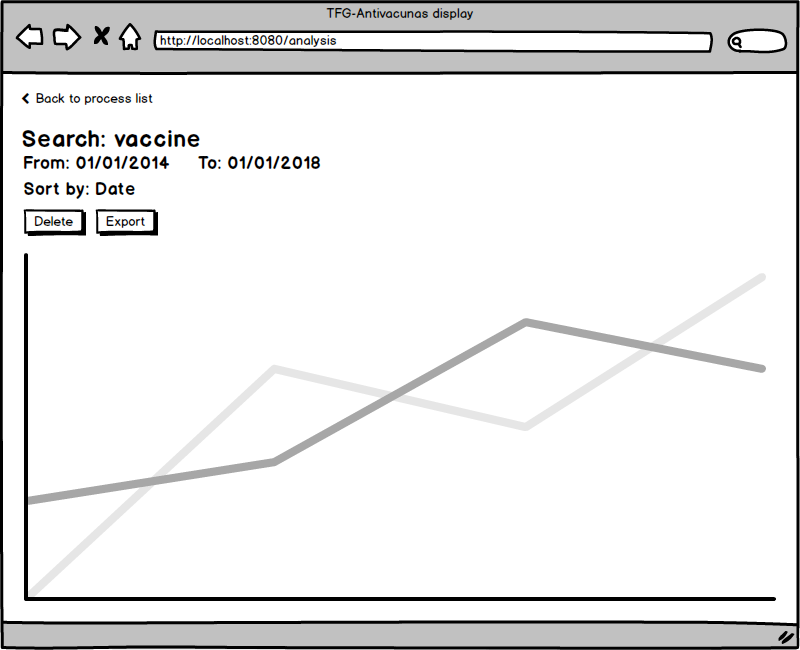
\includegraphics[width=60mm]{interfaz/04-05/2.png}}
\subfigure[\textit{YouTube} búsqueda vídeo relacionado]{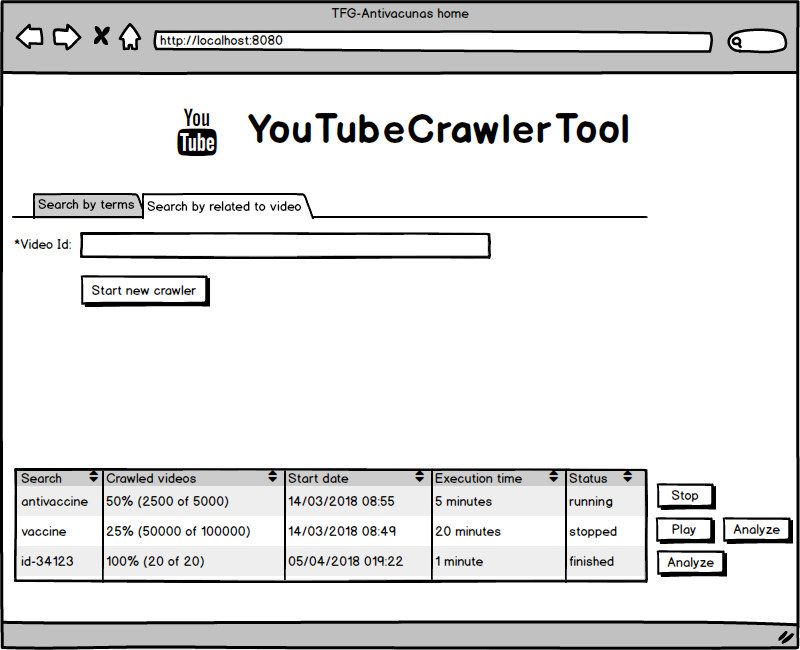
\includegraphics[width=60mm]{interfaz/04-05/3.png}}
\subfigure[\textit{YouTube} análisis vídeo relacionado]{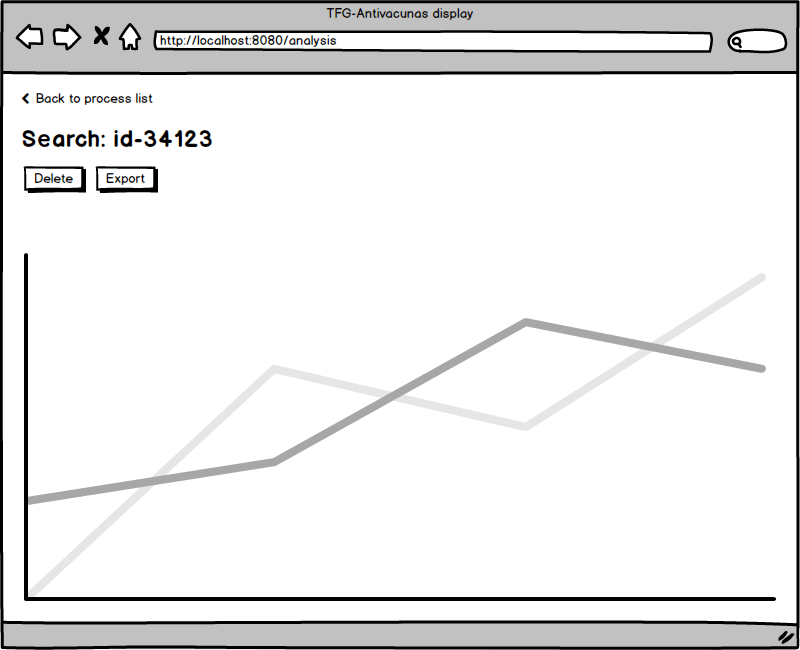
\includegraphics[width=60mm]{interfaz/04-05/4.png}}
\caption{Segunda propuesta interfaz de usuario}
\end{figure}

\noindent\textbf{Tercera y ultima propuesta presentada el 15/04/2018:}

\begin{figure}[H]
\centering
\subfigure[Login]{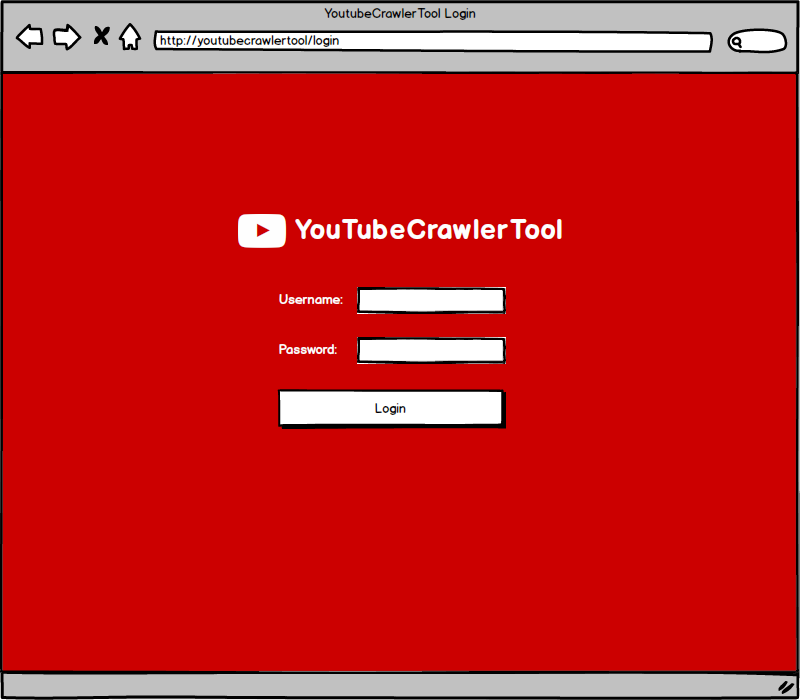
\includegraphics[width=60mm]{interfaz/04-15/1.png}}
\subfigure[Procesos de recolección]{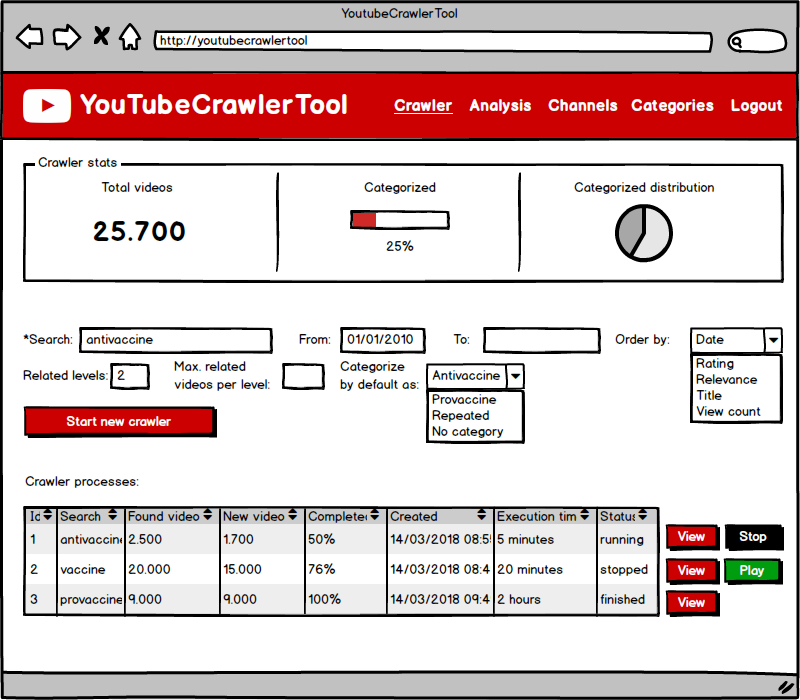
\includegraphics[width=60mm]{interfaz/04-15/2.png}}
\end{figure}
\begin{figure}[H]
\centering
\subfigure[Proceso de recolección]{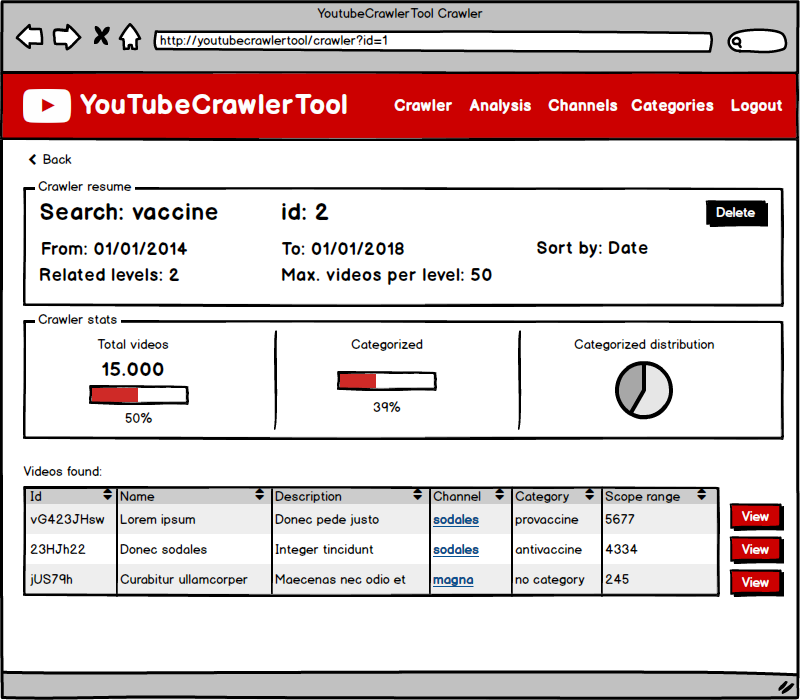
\includegraphics[width=60mm]{interfaz/04-15/3.png}}
\subfigure[Vista vídeo en detalle]{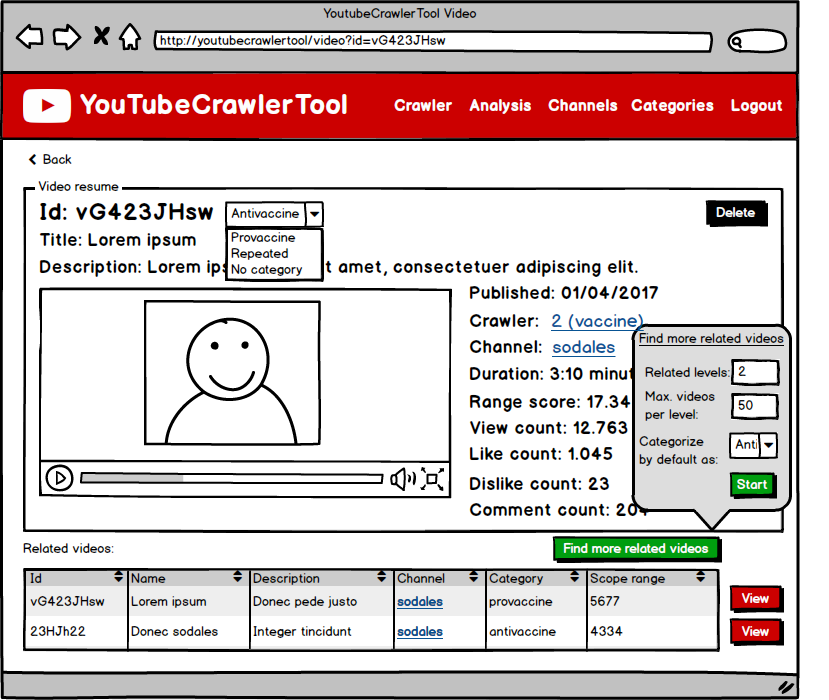
\includegraphics[width=60mm]{interfaz/04-15/4.png}}
\end{figure}
\begin{figure}[H]
\centering
\subfigure[Listado de canales]{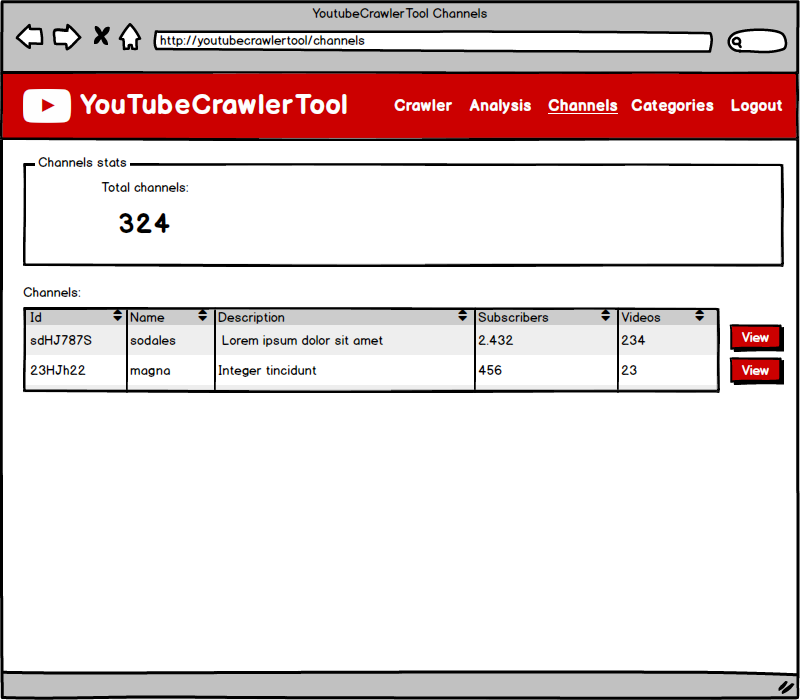
\includegraphics[width=60mm]{interfaz/04-15/5.png}}
\subfigure[Vista canal en detalle]{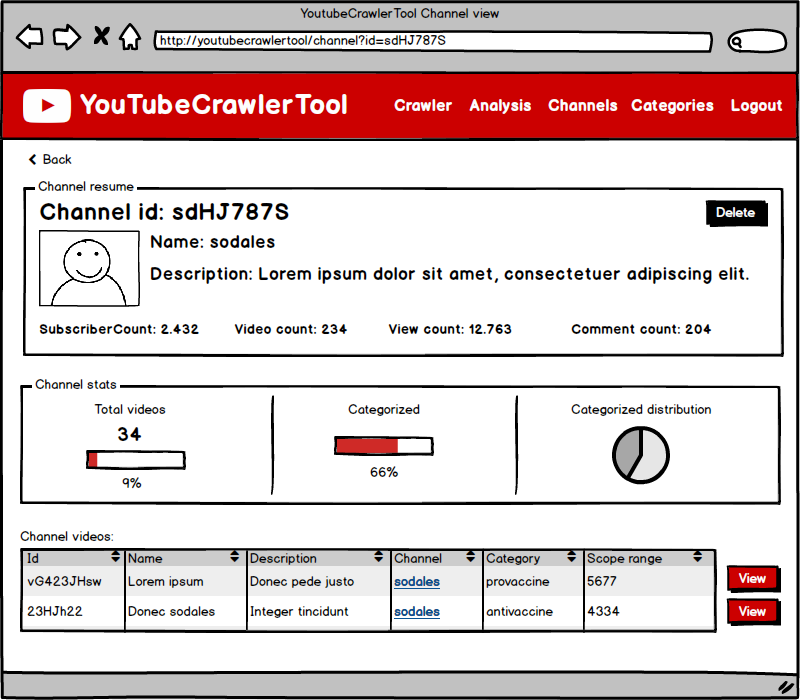
\includegraphics[width=60mm]{interfaz/04-15/6.png}}
\end{figure}
\begin{figure}[H]
\centering
\subfigure[Listado de categorías]{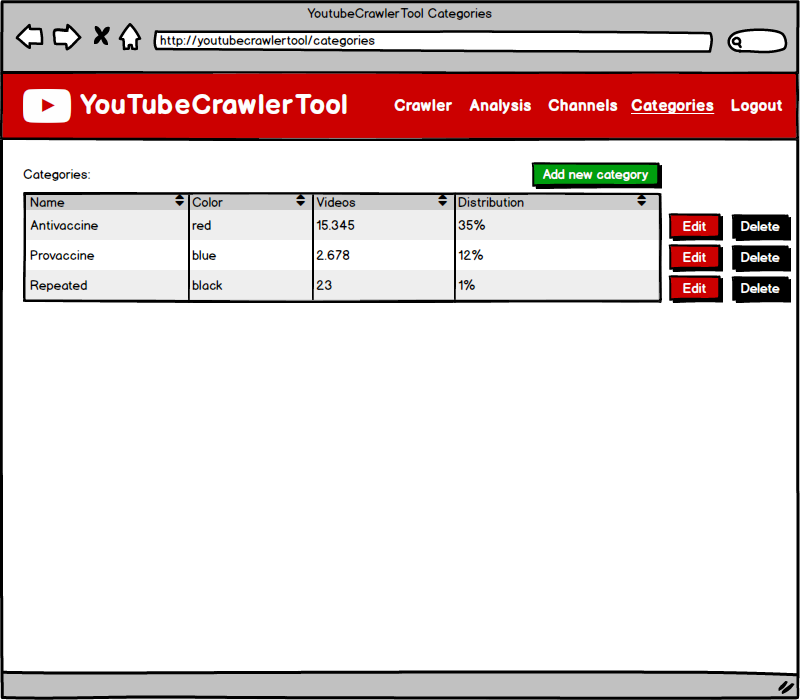
\includegraphics[width=60mm]{interfaz/04-15/7.png}}
\subfigure[Añadir nueva categoría]{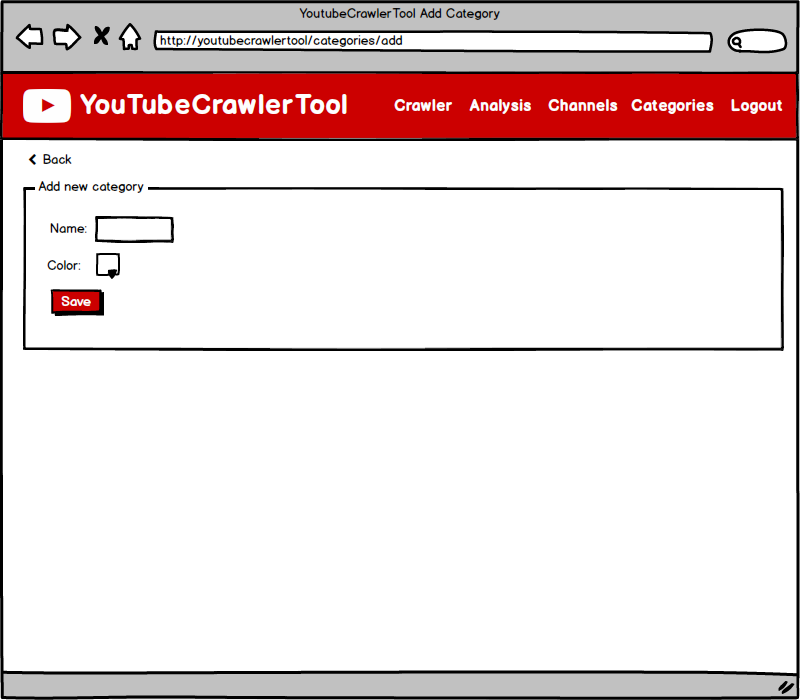
\includegraphics[width=60mm]{interfaz/04-15/8.png}}
\end{figure}
\begin{figure}[H]
\centering
\subfigure[Editar categoría]{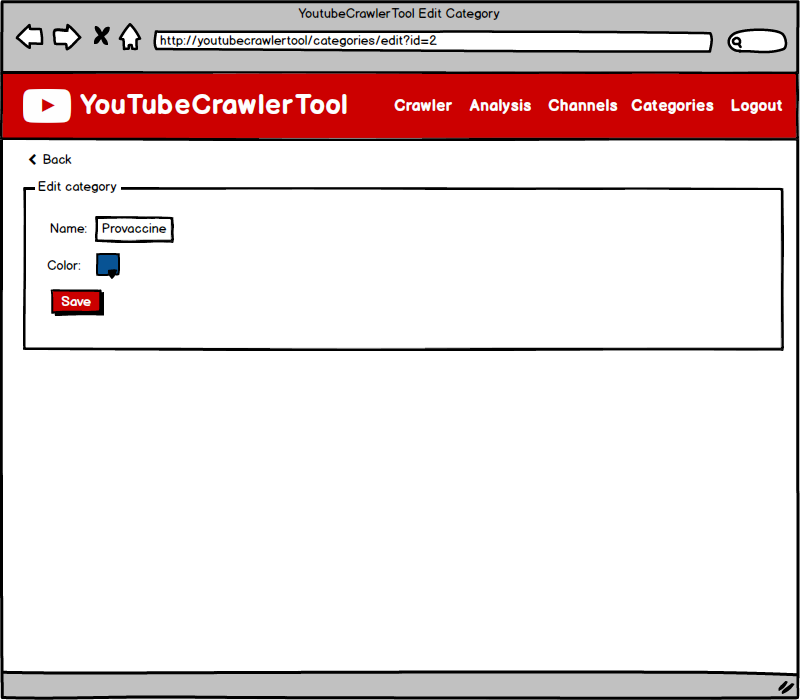
\includegraphics[width=60mm]{interfaz/04-15/9.png}}
\subfigure[Vista de análisis]{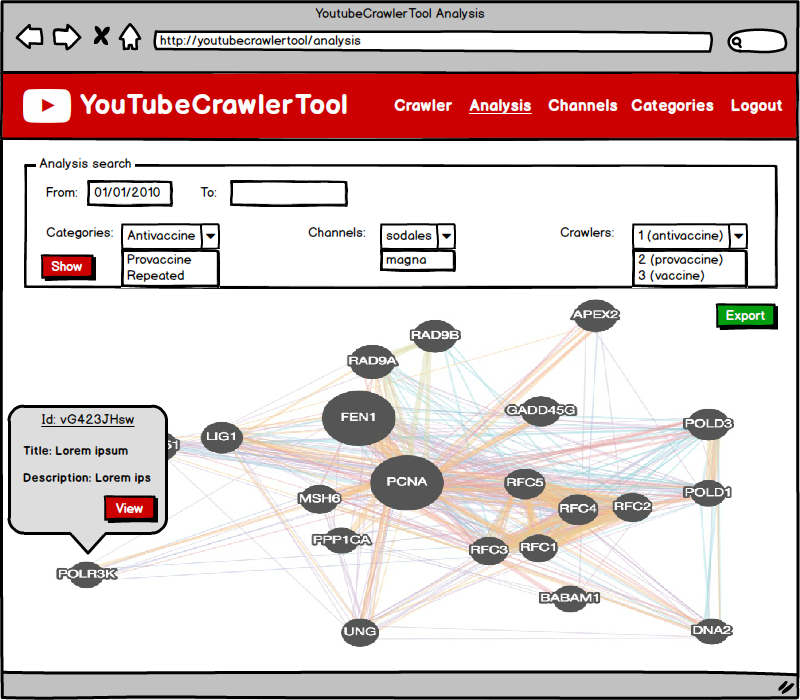
\includegraphics[width=60mm]{interfaz/04-15/10.png}}
\caption{Tercera y ultima propuesta de interfaz de usuario}
\end{figure}

Cabe destacar que, debido a iteraciones de desarrollo realizadas posteriormente a la presentación y aprobación de la ultima propuesta de interfaz de usuario presentada, esta no refleja el estado final de la aplicación.
\bigskip 

\subsection{Arquitectura WEB}
La decisión de realizar una aplicación Web viene motivada por las ventajas que aporta este medio en comparación con las aplicaciones de escritorio como por ejemplo, facilidades el trabajo colaborativo o centralizar la información y los procesos entre otros. Y de entre las diferentes arquitecturas Web, para el desarrollo del proyecto se escogió implementar una arquitectura REST por capas.
\\

REST (proveniente del acrónimo en ingles \textit{REpresentation State Transfer}) es un estilo arquitectónico en el desarrollo de aplicaciones Web que esta definido por una serie de principios. Algunos de los mas destacados son:
\begin{itemize}
\item Las solicitudes son sin estado.
\item Se sirven recursos, no funcionalidades (tales como objectos de base de datos).
\item Se accede a los recursos mediante URI que debe ser única por recurso.
\item Las operaciones sobre los recursos se realizan mediante HTTP especificando métodos estándar (tales como  \textit{GET}, \textit{PUT}, \textit{POST} y \textit{DELETE}).
\item Como formato para el intercambio de recursos se suele utilizar JSON o XML. 
\end{itemize}

La elección de esta arquitectura es a razón de los beneficios inherentes que aporta, tales como simplicidad en la arquitectura, escalable, extensible o la separación entre la capa de aplicación y capa de presentación. Gracias a esta arquitectura y de ser requerido en el futuro, ademas de disponer de un cliente Web como el diseñado en el proyecto actual, también seria factible, por ejemplo, proveer una aplicación móvil nativa sin tener que cambiar los servicios ofrecidos por el sistema.
\\

Como alternativa al uso de REST se considero utilizar una arquitectura basada en RPC. La gran diferencia entre ambas (entre otras) reside en el hecho que REST se centra en recursos mientras que RPC en funcionalidades. Por facilidad de uso y simplicidad se escogió implementar una arquitectura REST en detrimento de RPC.
\\

La aplicación de los principios REST conllevo a realizar otra decisión arquitectónica, dividir la aplicación por capas. En este caso, se escogió aplicar una arquitectura cliente-servidor de tres capas divididas en: 
\begin{itemize}
\item \textbf{Capa de datos}: Donde se persistirá la información de la aplicación utilizando un SGBD.
\item \textbf{Capa de aplicación}: En donde se llevara a cabo el acceso a datos, la lógica de negocio y de presentación que, a la vez, estará dividida entre el controlador de solicitudes de navegador (vistas HTML) y el controlador de solicitudes de recursos (API REST).
\item \textbf{Capa cliente}: Consistente en una interfaz de usuario web.
\end{itemize}

\begin{figure}[H]
\centering
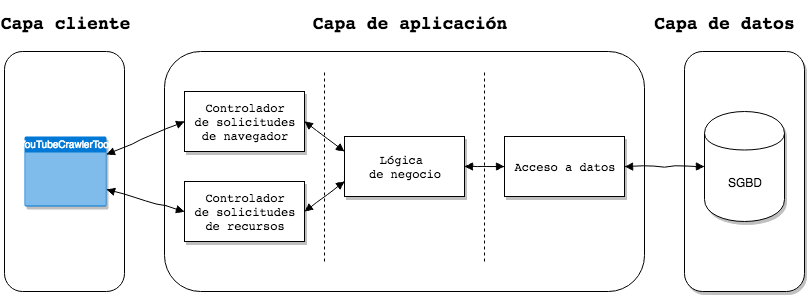
\includegraphics[scale=0.40]{diseno/ArquitecturaRESTPorCapas.png}
\caption{Arquitectura REST por capas}
\end{figure}

Gracias a esta distribución, se espera poder atorgar a la aplicación de una gran capacidad de reutilización y extensibilidad. En lo que ha distribución física se refiere, la capa cliente se ejecutara en los clientes Web de los usuarios y la capa de aplicación y de datos en un servidor. En los siguientes capítulos se detalla el diseño realizado para cada una de las capas.
\medskip 

\subsection{Diseño capa de datos}\label{disenoDatos} 
En la capa de datos es donde se persistirá la información necesaria para el funcionamiento de la aplicación. Para tales efectos haremos uso de un sistema gestor de base de datos (SGBD) donde la implementación escogida de la misma se detalla en el apartado \ref{sgbd}.
\\

Para diseñar la capa de datos se proporciono un diagrama UML de clases del esquema invariante de la información:

\begin{figure}[H]
\centering
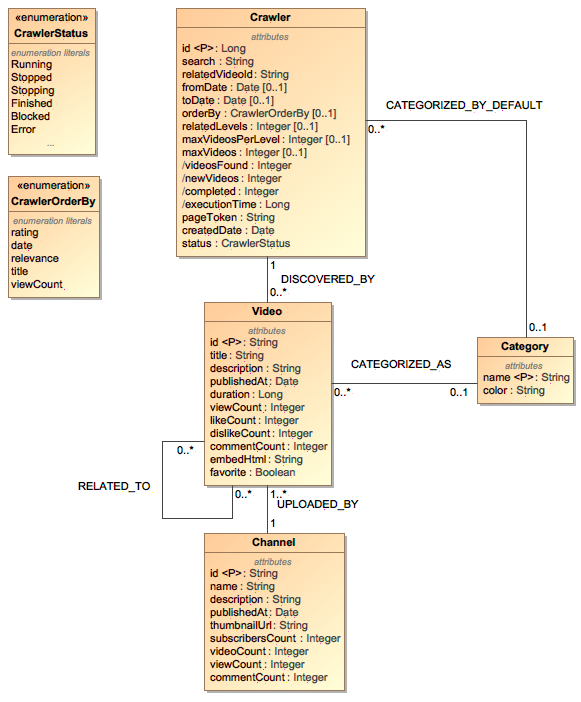
\includegraphics[scale=0.6]{diseno/DatabaseUML.png}
\caption{Diagrama de classes UML capa de datos}
\end{figure}

A continuación se detallan las entidades diseñadas:
\begin{itemize}
\item \textbf{\textit{Crawler}:} Representa a un proceso de recolección de vídeos y contiene, ademas de los criterios de búsqueda introducidos por el usuario, información sobre el estado y resultado del proceso. Un proceso de recolección puede tener asignada una categoría por defecto y haber recolectado varios vídeos.
\item \textbf{\textit{Video}:} Representa un vídeo en la red social \textit{YouTube}. Un vídeo puede tener asignada una categoría, ha sido recolectado por un proceso de recolección, ha sido publicado por un canal y puede estar relacionado con otros vídeos.
\item \textbf{\textit{Channel}:} Representa a un canal de publicación de vídeos en la red social \textit{YouTube}. Un canal puede haber publicado varios vídeos.
\item \textbf{\textit{Category}:} Representa una categoría creada por el usuario de la aplicación. Una categoría puede etiquetar varios vídeos y puede estar asignada por defecto en varios procesos de recolección.
\end{itemize}

\medskip 

\subsection{Diseño capa de aplicación}\label{capaAplicacion} 
Para el diseño de la capa de aplicación se decidió definir un componente por cada grupo de funcionalidad identificada en los casos de uso definidos en el apartado \ref{casosDeUso}. En concreto, los componentes diseñados fueron los siguientes:

\begin{itemize}
\item \textbf{\textit{Crawler}:} Agrupa la funcionalidad del recolector de vídeos.
\item \textbf{\textit{Video}:} Agrupa la funcionalidad relacionada con la entidad \textit{video}.
\item \textbf{\textit{Channel}:} Agrupa la funcionalidad relacionada con la entidad \textit{channel}.
\item \textbf{\textit{Category}:} Agrupa la funcionalidad relacionada con la entidad \textit{category}.
\item \textbf{\textit{Analysis}:} Agrupa la funcionalidad relacionada con la visualización en formato de grafo y exportación a fichero csv.
\end{itemize}

En donde en cada capa de la aplicación podemos encontrar representado el diseño realizado de cada componente.
\\

A continuación se facilita la figura donde se representa el diagrama de componentes de la aplicación al completo y en próximos apartados se detallan cada una de las capas juntos con los diferentes diagrama refinados:
\newpage 

\begin{figure}[H]
\centering
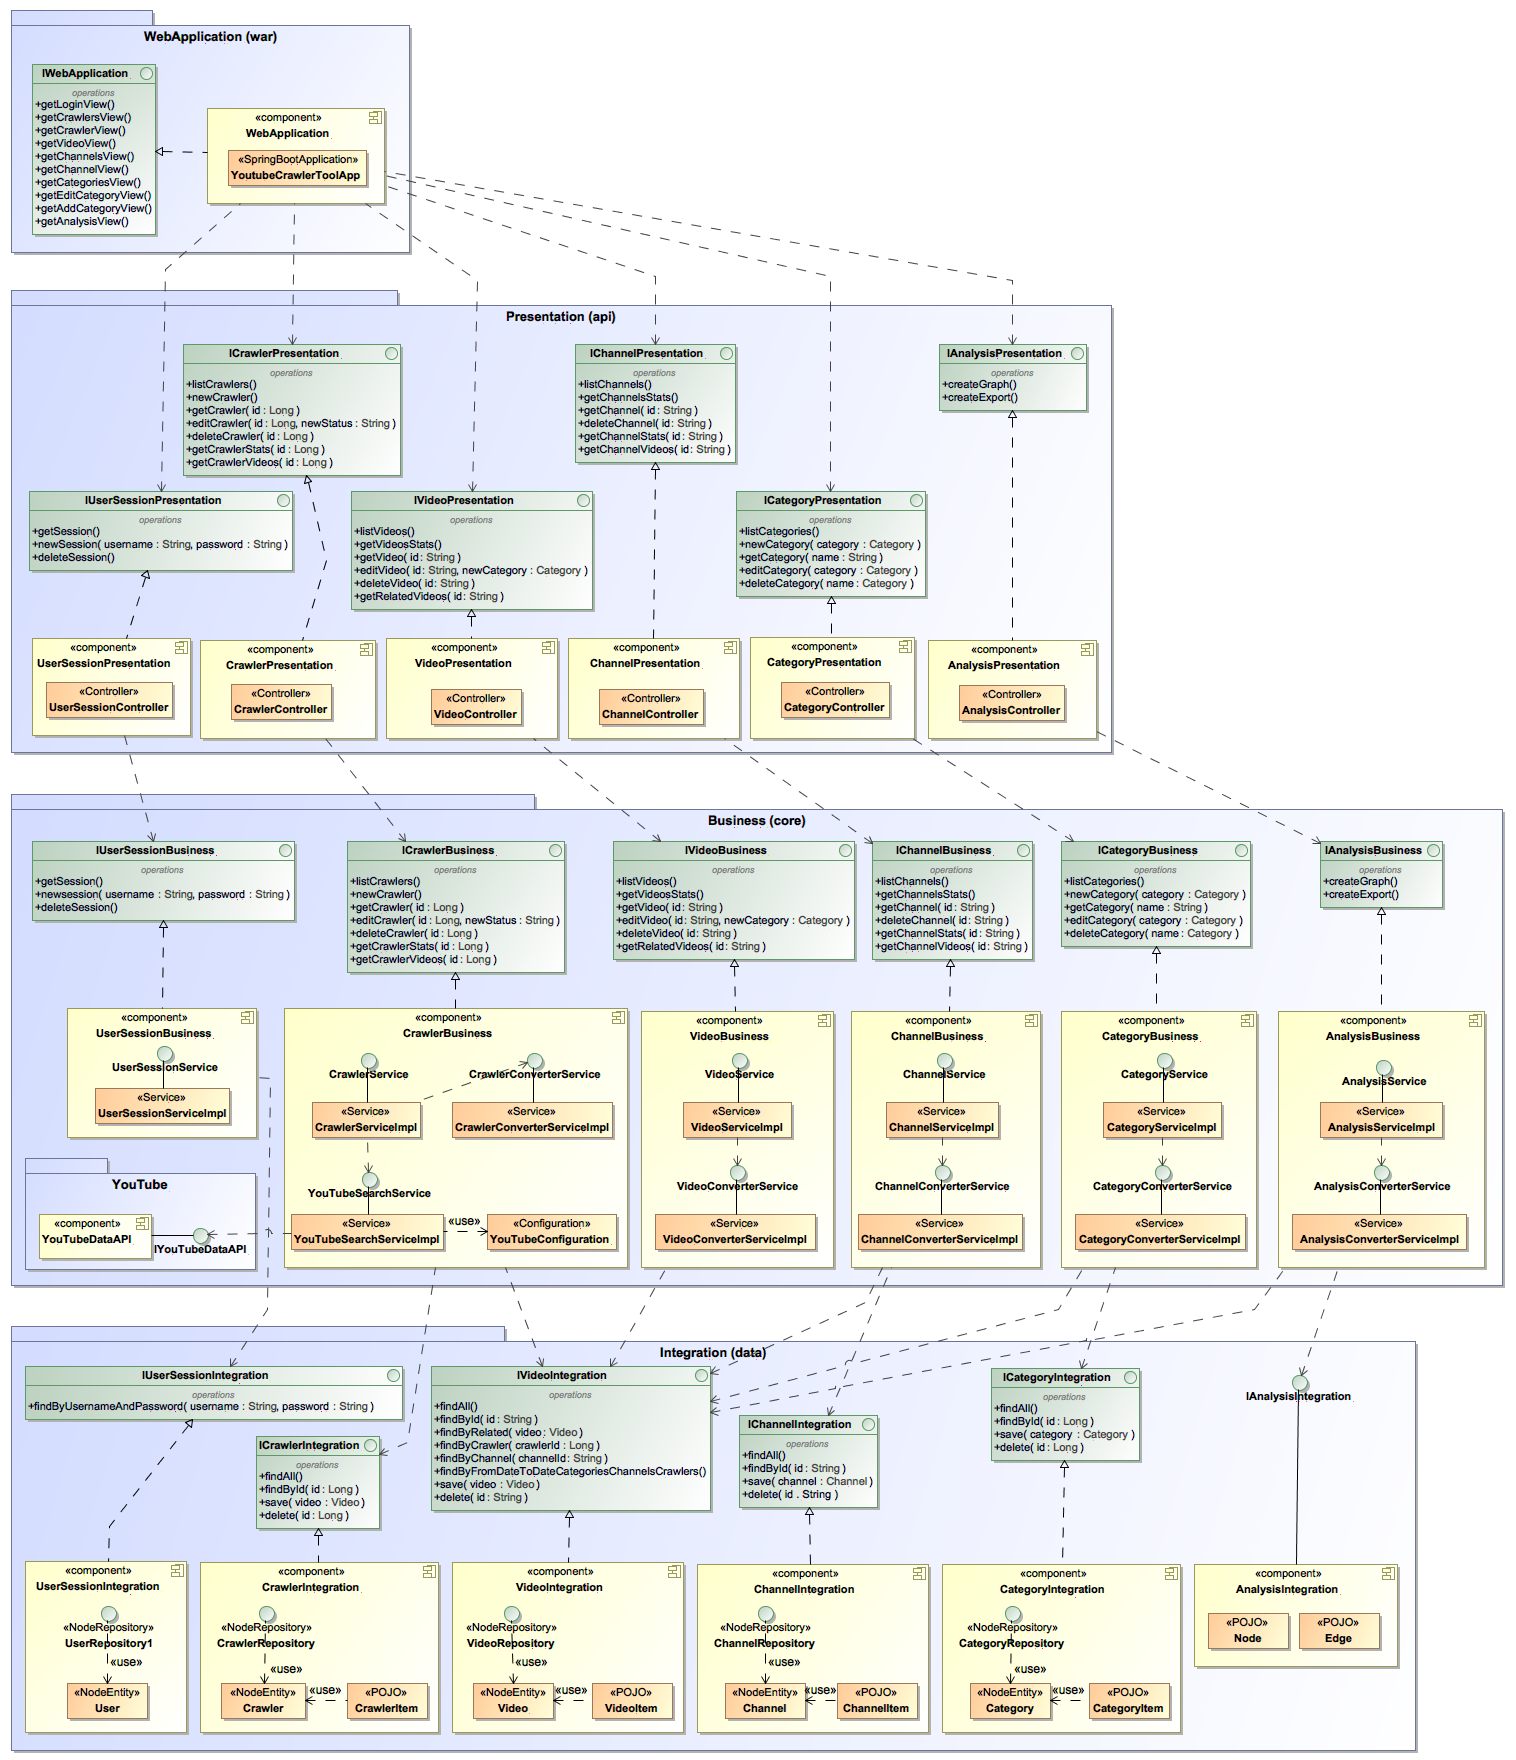
\includegraphics[scale=0.27]{diseno/ComponentDiagram3.png}
\caption{Diagrama de componentes}
\end{figure}
\newpage 

\subsubsection{Capa de acceso a datos}
Esta capa es la encargada de proporcionar acceso a la aplicación a los datos realizando y gestionando las conexiones y peticiones al SGDB.
\\


\noindent\textbf{Definición de componentes}
\begin{figure}[H]
\centering
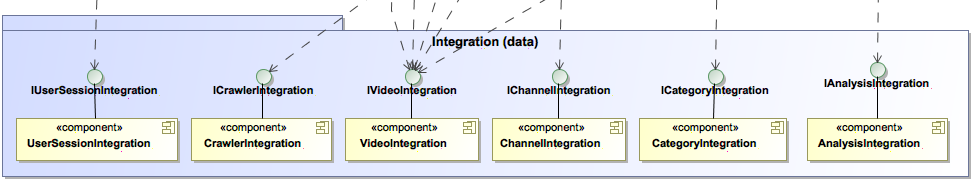
\includegraphics[scale=0.35]{diseno/accesoDatos/ComponentsDiagram.png}
\caption{Diagrama de componentes capa acceso a datos - componentes}
\end{figure}

\noindent\textbf{Definición de interfaces}
\begin{figure}[H]
\centering
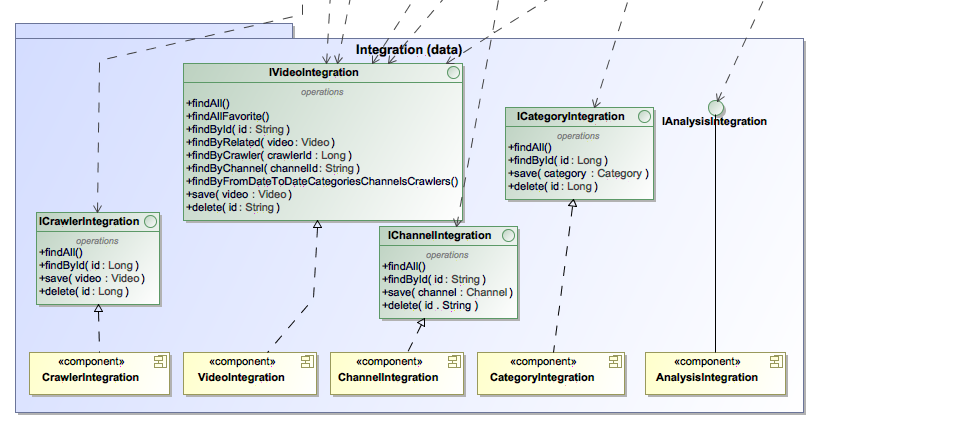
\includegraphics[scale=0.3]{diseno/accesoDatos/ComponentDiagram2.png}
\caption{Diagrama de componentes capa acceso a datos - interfaces}
\end{figure}

\noindent\textbf{Definición de implementaciones}
\begin{figure}[H]
\centering
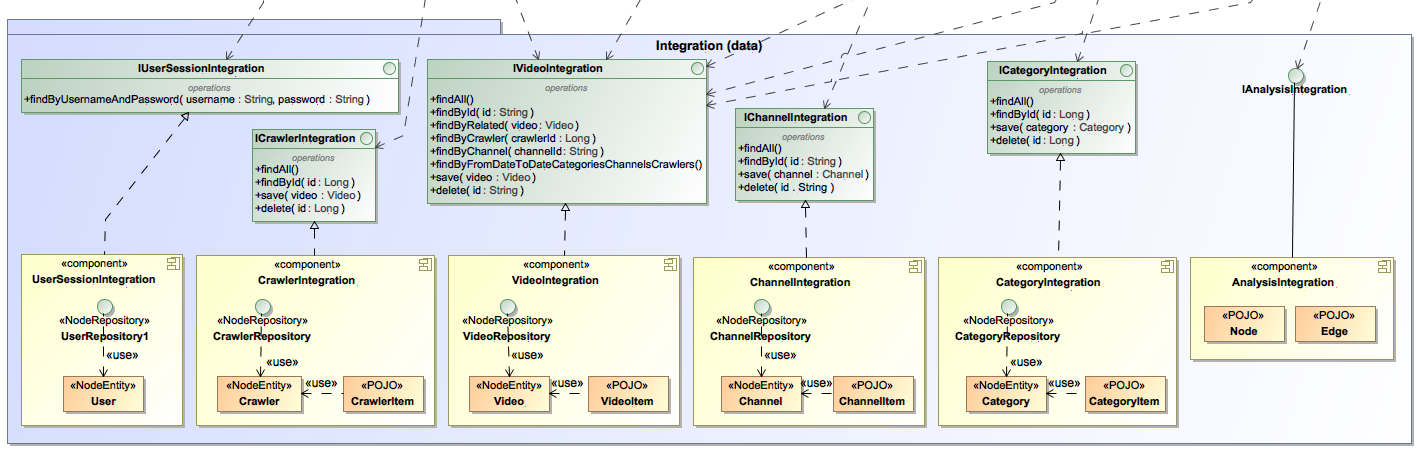
\includegraphics[scale=0.25]{diseno/accesoDatos/ComponentDiagram3.png}
\caption{Diagrama de componentes capa acceso a datos - implementaciones}
\end{figure}

\medskip 

\subsubsection{Capa de lógica de negocio}
La capa de lógica de negocio es la encarga de actuar como mediadora entre la capa de acceso a datos y la capa de presentación añadiendo la lógica necesaria sobre los datos que los requerimientos de la aplicación necesiten. Es en esta capa también, donde se realizara la conexión con el servicio externo en forma de API  de \textit{YouTube} para obtener los vídeos.
\\

\noindent\textbf{Definición de componentes}
\begin{figure}[H]
\centering
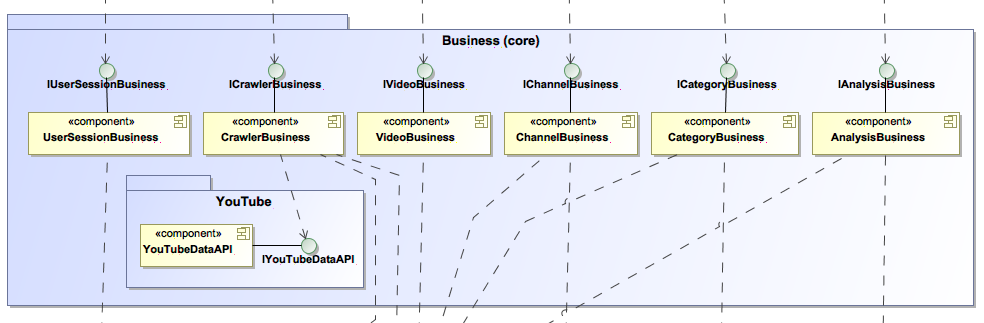
\includegraphics[scale=0.35]{diseno/negocio/ComponentsDiagram.png}
\caption{Diagrama de componentes capa de lógica de negocio - componentes}
\end{figure}

\noindent\textbf{Definición de interfaces}
\begin{figure}[H]
\centering
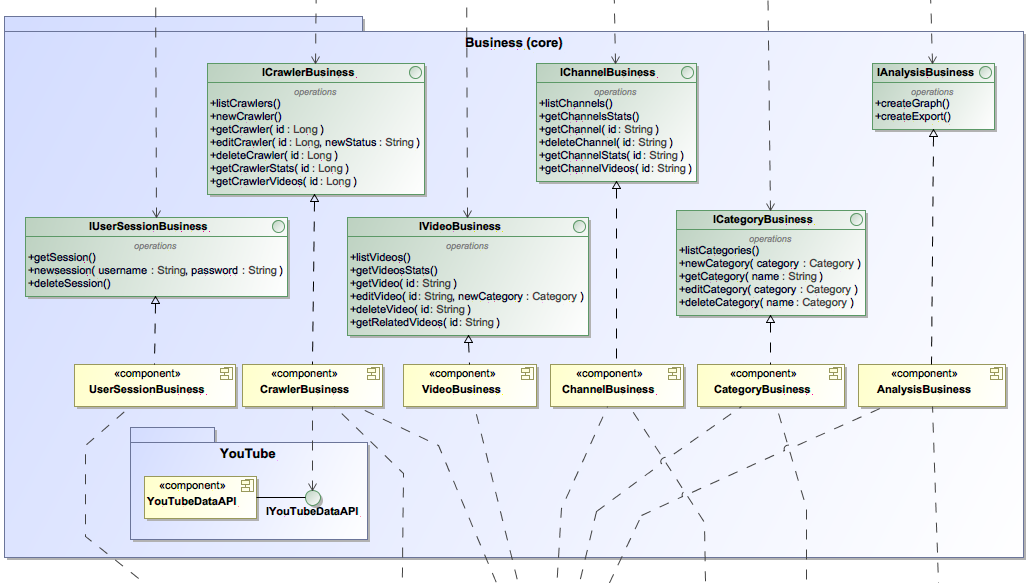
\includegraphics[scale=0.3]{diseno/negocio/ComponentDiagram2.png}
\caption{Diagrama de componentes capa de lógica de negocio - interfaces}
\end{figure}
\newpage 

\noindent\textbf{Definición de implementaciones}
\begin{figure}[H]
\centering
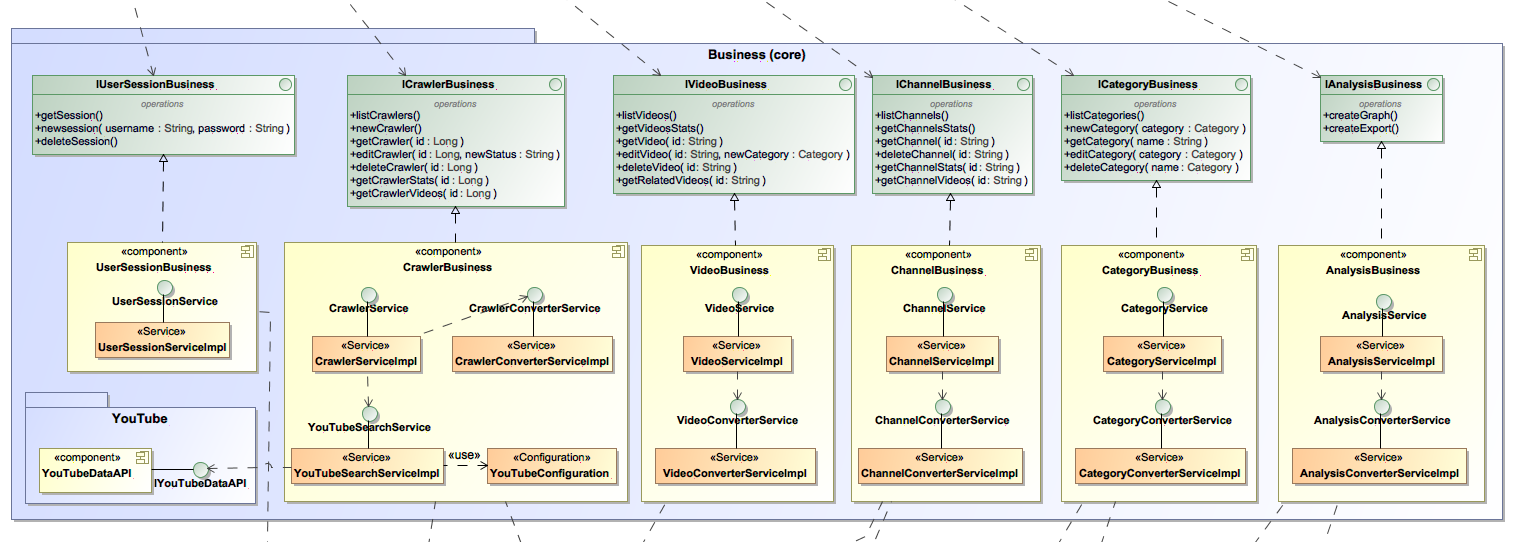
\includegraphics[scale=0.25]{diseno/negocio/ComponentDiagram3.png}
\caption{Diagrama de componentes capa de lógica de negocio - implementaciones}
\end{figure}

\medskip 

\subsubsection{Capa de presentación}
En la capa de presentación es donde habitan el controlador de solicitudes de recursos (paquete '\textit{Presentation (api)}') y el controlador de solicitudes de navegador (paquete '\textit{WebApplication (war)}') aplicando el patrón modelo vista controlador (MVC) \cite{19}.
\\

\noindent\textbf{Definición de componentes}
\begin{figure}[H]
\centering
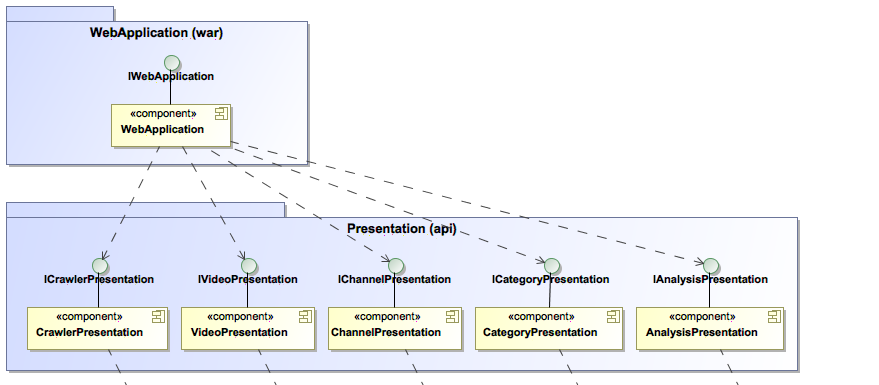
\includegraphics[scale=0.35]{diseno/presentacion/ComponentsDiagram.png}
\caption{Diagrama de componentes capa de presentación - componentes}
\end{figure}
\newpage 

\noindent\textbf{Definición de interfaces}
\begin{figure}[H]
\centering
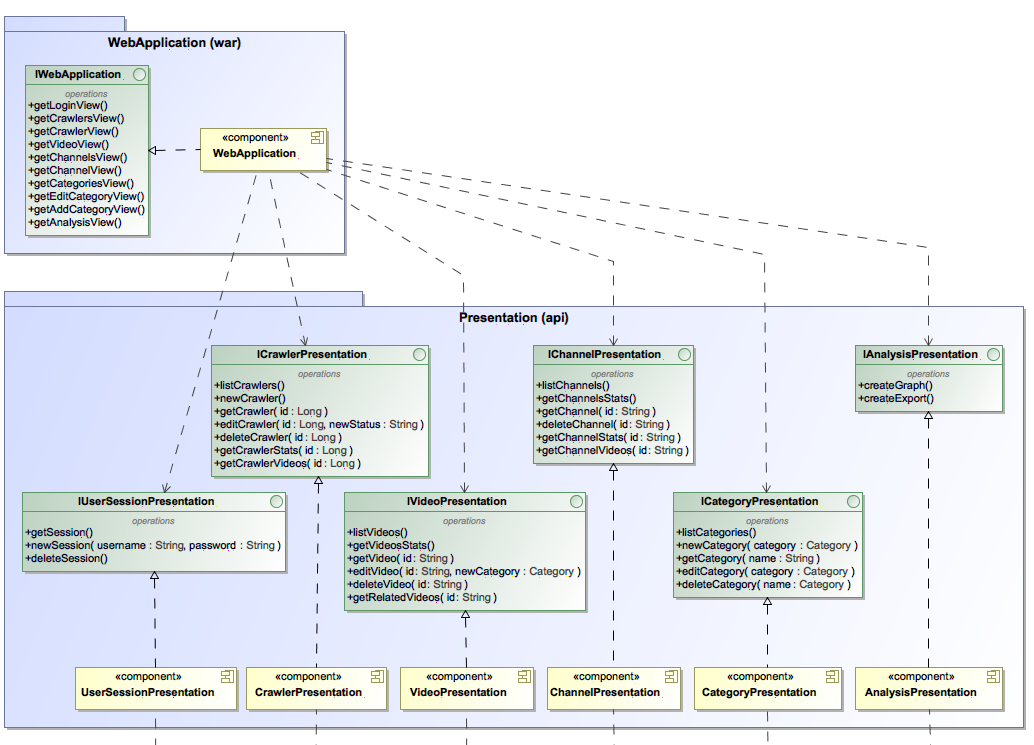
\includegraphics[scale=0.3]{diseno/presentacion/ComponentDiagram2.png}
\caption{Diagrama de componentes capa de presentación - interfaces}
\end{figure}

\noindent\textbf{Definición de implementaciones}
\begin{figure}[H]
\centering
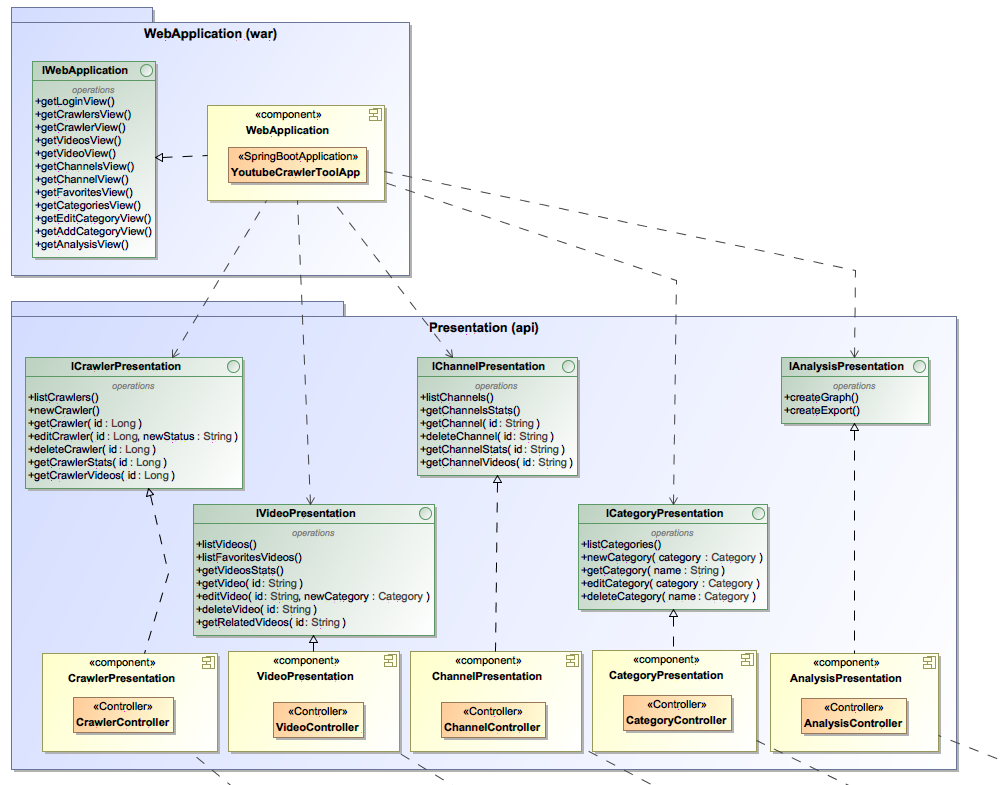
\includegraphics[scale=0.25]{diseno/presentacion/ComponentDiagram3.png}
\caption{Diagrama de componentes capa de presentación - implementaciones}
\end{figure}

\subsubsection{API REST}\label{rest} 
A continuación se facilita el diseño realizado de la API REST de la aplicación detallando la URI del recurso, el método de ejecución y una breve descripción.
\\

La API se ha diseñado respetando los patrones de diseño definidos por la arquitectura REST \cite{20}:
\\

\noindent\textbf{Componente \textit{crawler}:}
\begin{table}[H]
\centering
\resizebox{\textwidth}{!}{%
\begin{tabular}{|l|l|l|}
\hline
\textbf{Metodo} & \textbf{Uri}            & \textbf{Descripción}                                               \\ \hline
GET             & api/crawlers               & Lista todos los procesos de recolección.                           \\ \hline
POST            & api/crawlers               & Inicia un nuevo proceso de recolección. Requiere autentificación.  \\ \hline
GET             & api/crawlers/\{id\}        & Devuelve un proceso de recolección.                                \\ \hline
PUT             & api/crawlers/\{id\}        & Editar un proceso de recolección. Requiere identificación.        \\ \hline
DELETE          & api/crawlers/\{id\}        & Borra un proceso de recolección. Requiere identificación.         \\ \hline
GET             & api/crawlers/\{id\}/stats  & Devuelve las estadísticas de un proceso de recolección.            \\ \hline
GET             & api/crawlers/\{id\}/videos & Lista todos los vídeos descubiertos por un proceso de recolección. \\ \hline
\end{tabular}%
}
\caption{Componente \textit{crawler} API}
\end{table}

\noindent\textbf{Componente \textit{video}:}
\begin{table}[H]
\centering
\resizebox{\textwidth}{!}{%
\begin{tabular}{|l|l|l|}
\hline
\textbf{Metodo} & \textbf{Uri}             & \textbf{Descripción}                              \\ \hline
GET             & api/videos               & Lista todos los vídeos.                           \\ \hline
GET             & api/videos/stats         & Devuelve las estadísticas de todos los vídeos.    \\ \hline
GET             & api/videos/favorites     & Devuelve los vídeos favoritos.                    \\ \hline
GET             & api/videos/\{id\}        & Devuelve un vídeo.                                \\ \hline
PUT             & api/videos/\{id\}        & Editar un vídeo. Requiere identificación.         \\ \hline
DELETE          & api/videos/\{id\}        & Borra un vídeo. Requiere identificación.          \\ \hline
GET             & api/videos/\{id\}/videos & Lista todos los vídeos relacionados con un vídeo. \\ \hline
\end{tabular}%
}
\caption{Componente \textit{video} API}
\end{table}

\noindent\textbf{Componente \textit{channel}:}
\begin{table}[H]
\centering
\resizebox{\textwidth}{!}{%
\begin{tabular}{|l|l|l|}
\hline
\textbf{Metodo} & \textbf{Uri}               & \textbf{Descripción}                              \\ \hline
GET             & api/channels               & Lista todos los canales                           \\ \hline
GET             & api/channels/\{id\}        & Devuelve un canal.                                \\ \hline
DELETE          & api/channels/\{id\}        & Borra un canal. Requiere identificación            \\ \hline
GET             & api/channels/\{id\}/stats  & Devuelve la estadísticas de un canal              \\ \hline
GET             & api/channels/\{id\}/videos & Lista todos los vídeos relacionados con un canal. \\ \hline
\end{tabular}%
}
\caption{Componente \textit{channel} API}
\end{table}
\newpage 

\noindent\textbf{Componente \textit{category}:}
\begin{table}[H]
\centering
\resizebox{\textwidth}{!}{%
\begin{tabular}{|l|l|l|}
\hline
\textbf{Metodo} & \textbf{Uri}                   & \textbf{Descripción}                                    \\ \hline
GET             & api/categories                 & Lista todas las categorías                              \\ \hline
POST            & api/categories                 & Crea una nueva categoría. Requiere identificación.      \\ \hline
GET             & api/categories/\{name\}        & Devuelve una categoría.                                 \\ \hline
PUT             & api/categories/\{name\}        & Editar una categoría. Requiere identificación.          \\ \hline
DELETE          & api/categories/\{name\}        & Borra una categoría.                                    \\ \hline
GET             & api/categories/\{name\}/stats  & Devuelve las estadísticas de una categoría.             \\ \hline
GET             & api/categories/\{name\}/videos & Lista todos los vídeos categorizados por una categoría. \\ \hline
\end{tabular}%
}
\caption{Componente \textit{category} API}
\end{table}

\noindent\textbf{Componente \textit{analysis}:}
\begin{table}[H]
\centering
\resizebox{\textwidth}{!}{%
\begin{tabular}{|l|l|l|}
\hline
\textbf{Metodo} & \textbf{Uri} & \textbf{Descripción}                                           \\ \hline
POST            & api/graphs   & Crea un nuevo grafo (no se persiste, se muestra por pantalla). \\ \hline
\end{tabular}%
}
\caption{Componente \textit{analysis} API}
\end{table}

\medskip 

\subsection{Diseño capa cliente}\label{capaCliente} 
Finalmente, para el diseño de la capa cliente correspondiente a la interfaz de usuario de la aplicación web, se especificaron las vistas de acuerdo con los casos de uso definidos en el apartado \ref{casosDeUso} y a la propuesta de interfaz de usuario aprobada por la clienta \ref{propuestaInterfazUsuario}:
\\

\begin{itemize}
\item \textbf{\textit{loginView.html}:} Permite la identificación en el sistema.
\item \textbf{\textit{crawlersView.html}:} Pagina principal de la aplicación. Lista los procesos de recolección existentes y permite gestionarlos y iniciar nuevos procesos.
\item \textbf{\textit{crawlerView.html}:} Vista detalle de un proceso de recolección.
\item \textbf{\textit{videosView.html}:} Listado de todos los vídeos del sistema.
\item \textbf{\textit{videoView.html}:} Vista detalle de un vídeo.
\item \textbf{\textit{channelsView.html}:} Lista de todos los canales del sistema.
\item \textbf{\textit{channelView.html}:} Vista detalle de un canal.
\item \textbf{\textit{analysisView.html}:} Permite visualizar los vídeos en un grafo y exportarlos a fichero csv.
\item \textbf{\textit{favoriteVideosView.html}:} Listado de todos los vídeos favoritos.
\item \textbf{\textit{categoriesView.html}:} Lista todas las categorías del sistema.
\item \textbf{\textit{addCategoryView.html}:} Permite crear una nueva categoría.
\item \textbf{\textit{editCategoryView.html}:} Permite editar una categoría.
\end{itemize}

Dichas vistas serán gestionadas por el controlador de solicitudes de navegador y en ellas, se realizaran peticiones asíncronas a recursos utilizando la API REST de la aplicación que sera gestionada por el controlador de solicitudes de recursos.
\\

La figura a continuación ejemplifica el mapa web de la aplicación con los flujos de interacción posibles y funcionalidades previstas para cada vista:

\begin{figure}[H]
\centering
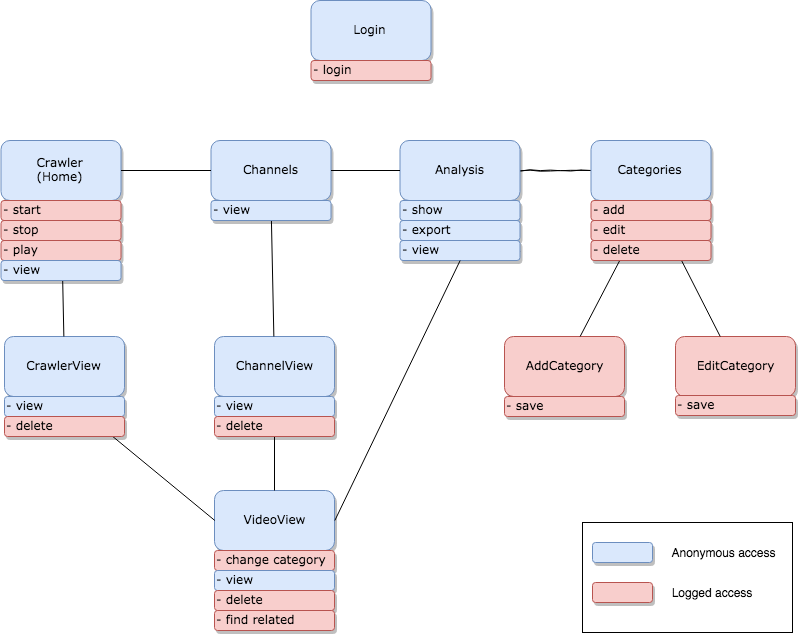
\includegraphics[scale=0.40]{diseno/capaCliente.png}
\caption{Diseño vistas capa cliente}
\end{figure}

\newpage 



\section{Desarrollo}
El código fuente de la aplicación desarrollada la cual se detalla a continuación, se encuentra disponible en un repositorio publico de \textit{GitHub}: \href{https://github.com/jsanchezmend/TFGAntivacunas/tree/master/YouTubeCrawlerTool}{YouTubeCrawlerTool}.
\bigskip

\subsection{Entorno de desarrollo}\label{entorno} 
A continuación se detalla la configuración del entorno de desarrollo utilizada en el desarrollo del proyecto. Algunas de las cuales no representan obligatoriedad siendo posible utilizar alternativas diferentes con los mismos resultados, en este caso solo se pretende exponer la configuración utilizada:

\begin{itemize}
\item \textbf{Sistema operativo:} MacOS.
\item \textbf{Neo4J 3.3.5 Server Community version:} Instalación de servidor de base de datos Neo4J en local necesario para el desarrollo de la capa de datos.
\item \textbf{Java JDK 8:} Kit de desarrollo de Java versión 8 \cite{21} necesario para el desarrollo de la capa de aplicación.
\item \textbf{Git y creación de cuenta en GitHub:} Como herramienta para el control de versiones se ha escogido Git \cite{22}. Ademas, se creo una cuenta con perfil público en Github accesible desde el siguiente enlace: \url{https://github.com/jsanchezmend/TFGAntivacunas}.
\item \textbf{Maven:} Herramienta para la gestión de proyectos Java \cite{23}, fue utilizada para la construcción del proyecto y para la gestión de dependencias.
\item \textbf{Spring Tool Suite:} Entorno de desarrollo utilizado el cual se basa en una customización de Eclipse \cite{24}.
\item \textbf{Tomcat:} Para probar la aplicación se utilizo el servidor de aplicaciones Tomcat \cite{25}, pero devido al uso de Spring Boot \cite{26} no fue necesario realizar su instalación al incorporar esta solución una versión de Tomcat.
\item \textbf{Google API Key:} Para poder realizar consultas a la API de \textit{YouTube} es necesario obtener una clave de API que tendrá que ser utilizada cada vez que se haga uso de sus servicios. Para obtenerla, primero hay que acceder a la consola de desarrollo de \textit{Google} utilizando una cuenta previamente existente, crear un nuevo proyecto de desarrollo y activar los servicios de \textit{YouTube Data API v3} \cite{27}.
\end{itemize}
\medskip 

\subsection{Decisiones previas al desarrollo}
Antes de empezar con el desarrollo de la aplicación, fue necesario realizar algunas decisiones previas las cuales tendrían repercusión en la implementación final de la solución.  Para ayudar en la toma de decisión y estudiar la viabilidad de las mismas, estas fueron respaldadas con pruebas de concepto detalladas en la sección \ref{pocs}.
\\

En los próximos apartados se detallan algunas de las decisiones mas relevantes que se tuvieron que tomar, como fue el estudio y elección de la API de YouTube a consumir y el SGDB a utilizar. 
\medskip

\subsubsection{YouTube Data API}\label{youTubeDataAPI} 
Para ofrecer sus servicios a terceros, \textit{YouTube} divide su funcionalidad en cuatro grupos de APIs distintas dentro de la plataforma \textit{Google APIs}:

\begin{itemize}
\item \textbf{\textit{YouTube Data API v3}:} Proporciona acceso y servicios de búsqueda a recursos tales como vídeos, canales, comentarios entre otros.
\item \textbf{\textit{YouTube Analytics API}:} Permite obtener información analítica sobre la cuenta de un usuario, tales como número de suscripciones o número de visualizaciones entre otros. Este servicio esta limitado a uso personal, siendo solo posible acceder a la información del propio usuario que realiza la petición y no es permitido realizar consultas sobre otros usuarios.
\item \textbf{\textit{YouTube Reporting API}:} Complementaria a la \textit{YouTube Analytics API}, esta API permite al usuario de \textit{YouTube} programar la generación de informes sobre su información analítica. De igual forma que su antecesora, su eso esta limitado al uso personal.
\item \textbf{\textit{YouTube Ad Reach API}:} Dedicada a anunciantes, permite el estudio del alcance obtenido por campaña de publicidad.
\end{itemize}

\begin{figure}[H]
\centering

\includegraphics[scale=0.35]{desarrollo/youTubeAPI.png}
\caption{\textit{YouTube} APIs}
\end{figure}
\newpage 

Así entonces y según lo expuesto, para poder realizar búsquedas y obtener los contenidos que sean requeridos por el usuario, la aplicación hara uso de los servicios web expuestos por la \textit{YouTube Data API v3} \cite{29}.
\\

Dichos servicios se dividen por tipos de recursos a los cuales acceder, en donde cada recurso representa un tipo de contenido de \textit{YouTube} tales como vídeos, canales, listas de reproducción entre otros. Para poder obtener dichos recursos primeramente es necesario conocer los identificadores de los objectos que se quieren obtener, en donde para tales efectos hay habilitado un servició el propósito del cual es la obtención de dichos identificadores. Las únicas operaciones que se realizan en la aplicación son de lectura de recursos, no se requiere realizar operaciones de escritura. Así entonces, el modo en que nuestra aplicación utiliza estos servicios es de la siguiente forma:
\\
\begin{itemize}
\item \textbf{1- Obtención de identificadores de vídeos:} Se realiza una búsqueda para obtener los identificadores de los vídeos que se correspondan con los criterios de búsqueda introducidos por el usuario. Los resultados obtenidos, dependiendo del volumen de coincidencias que la búsqueda haya producido, podrán ser paginados requiriendo realizar peticiones iterativas para obtener los consiguientes resultados. El servició utilizado es el de \textit{'Seach'} y concretamente la operación \textit{'list'} \cite{30}.
\item \textbf{2- Obtención de vídeos:} Una vez obtenidos los identificadores de los vídeos que se quieren recuperar, se realiza una petición a la operación \textit{'list'} del servicio \textit{'Videos'} \cite{31} con dichos identificadores para obtener finalmente su contenido. De igual forma que en la obtención de identificadores, las peticiones a este servició se realizaran de forma iterativa para recuperar los vídeos de forma paginada.
\item \textbf{3- Obtención de canales:} Paralelamente a la obtención de vídeos para cada vídeo recuperado también se obtiene su canal. Para recuperarlo, de detectar que el canal en cuestión aun no se encuentra almacenado en el sistema, se realiza una petición al servicio \textit{'Channels'} operación \textit{'list'} \cite{32} con el identificador del canal obtenido en la información recuperada del vídeo.
\end{itemize}

Como se ha comentado en el apartado \ref{eleccionYouTube}, \textit{YouTube} define un sistema de cuotas en el uso de sus servicios, en el cual cada petición realizada tiene un coste que puede variar dependiendo del tipo de recurso y la información solicitada. Para minimizar el uso de cuota es importante solicitar solo los recursos y los campos que realmente sean necesarios para el usuario. A continuación se detalla el uso realizado para cada tipo de petición:
\\

\noindent\textbf{Obtención de identificadores de vídeos}\\
Petición HTTP: GET https://www.googleapis.com/youtube/v3/search\\

Criterios de búsqueda utilizados:
\begin{itemize}
\item \textbf{\textit{type}:} Permite escoger el tipo de recurso a recuperar. Valor utilizado por defecto \textit{'video'}.
\item \textbf{\textit{relevanceLanguage}:} Permite obtener resultados que son mas relevantes en el idioma introducido. Valor utilizado por defecto \textit{'en'}.
\item \textbf{\textit{q}:} Se utiliza en caso de realizarse una búsqueda textual, permite buscar recursos que correspondan con el texto introducido. En el texto a buscar se pueden utilizar negaciones y conjunciones.
\item \textbf{\textit{relatedToVideoId}:} Alternativamente a la búsqueda textual, con este campo se puede realizar una búsqueda de contenidos que estén relacionados con el identificador solicitado.
\item \textbf{\textit{publishedBefore} y publishedAfter:} Permite acotar la búsqueda a realizar dentro de un rango de fechas determinado. 
\item \textbf{\textit{order}:} Permite ordenar los resultados obtenidos por varios criterios: por fecha, rating, relevancia, titulo y numero de visualizaciones. Por defecto, los resultados son ordenados por relevancia.
\item \textbf{\textit{maxResults}:} Máximo de resultados obtenidos por pagina. El máximo valor aceptado es 50.
\item \textbf{\textit{pageToken}:} Identifica la pagina de resultados que debe ser devuelta. Como respuesta a la petición de búsqueda, juntamente con los recursos solicitados se devuelven los campos \textit{'nextPageToken'} y \textit{'prevPageToken'}, con la información devuelta en estos campos es posible navegar hacia la siguiente pagina de resultados o hacia la anterior.
\end{itemize}

Campos solicitados:
\begin{itemize}
\item \textbf{\textit{id}:} Identificador de los vídeos encontrados.
\end{itemize}
\medskip 

\noindent\textbf{Obtención de vídeos}\\
Petición HTTP: GET https://www.googleapis.com/youtube/v3/videos\\

Criterios de búsqueda utilizados:
\begin{itemize}
\item \textbf{\textit{id}:} Listado separado por comas de los identificadores de vídeos a recuperar.
\end{itemize}
\pagebreak 

Campos solicitados:
\begin{itemize}
\item \textbf{\textit{id}:} Identificador de vídeo.
\item \textbf{\textit{snippet/title}:} Titulo del vídeo.
\item \textbf{\textit{snippet/description}:} Descripción del vídeo.
\item \textbf{\textit{snippet/publishedAt}:} Fecha de publicación del vídeo.
\item \textbf{\textit{snippet/channelId}:} Identificador del canal que ha publicado el vídeo.
\item \textbf{\textit{contentDetails/duration}:} Tiempo de duración del vídeo.
\item \textbf{\textit{statistics/viewCount}:} Número de visualizaciones del vídeo.
\item \textbf{\textit{statistics/likeCount}:} Número de 'me gusta' que ha recibido el vídeo.
\item \textbf{\textit{statistics/dislikeCount}:} Número de 'no me gusta' que ha recibido el vídeo.
\item \textbf{\textit{statistics/commentCount}:} Número de comentarios realizados sobre el vídeo.
\item \textbf{\textit{player/embedHtml}:} Reproductor del vídeo en un formato \textit{iframe} html.
\end{itemize}
\medskip 

\noindent\textbf{Obtención de canales}\\
Petición HTTP: GET https://www.googleapis.com/youtube/v3/channels\\

Criterios de búsqueda utilizados:
\begin{itemize}
\item \textbf{\textit{id}:} Identificador del canal recuperar.
\end{itemize}
\medskip 

Campos solicitados:
\begin{itemize}
\item \textbf{\textit{id}:} Identificador del canal.
\item \textbf{\textit{snippet/title}:} Titulo del canal.
\item \textbf{\textit{snippet/description}:} Descripción del canal.
\item \textbf{\textit{snippet/publishedAt}:} Fecha de publicación del canal.
\item \textbf{\textit{snippet/customUrl}:} Dirección url del canal.
\item \textbf{\textit{snippet/thumbnails/default/url}:} Dirección url de la imagen representativa del canal.
\item \textbf{\textit{statistics/viewCount}:} Número de visualizaciones del canal.
\item \textbf{\textit{statistics/commentCount}:} Número de comentarios que ha recibido el canal.
\item \textbf{\textit{statistics/subscriberCount}:} Número de suscripciones al canal.
\item \textbf{\textit{statistics/videoCount}:} Número de vídeos publicados por el canal.
\end{itemize}

Antes de la implementación final de la solución, para probar los servicios aquí detallados se realizo con éxito la siguiente prueba de concepto: \href{https://github.com/jsanchezmend/TFGAntivacunas/tree/master/POCYouTubeCrawler}{POCYouTubeCrawler}.

\medskip 

\subsubsection{Neo4j como SGBD}\label{sgbd} 
Como consecuencia de los requerimientos del proyecto y al futuro uso para el cual esta destinada la aplicación, se requiere el almacenamiento de grandes cantidades de información que pueden o no estar estructuradas y a las cuales se requiere una alta accesibilidad.
\\

Por estos motivos, como gestor de bases datos se considero el uso de bases de datos NoSQL en vez de hacer uso de una base de datos relacional. Entre las principales características que ofrecen las bases de datos NoSQL que provocaron su elección en el proyecto destacamos las siguientes:

\begin{itemize}
\item \textbf{Manejo de grandes cantidades de datos:} Las bases de datos NoSQL al no garantizar completamente las características ACID (atomicidad, consistencia, aislamiento y durabilidad) \cite{33}, permiten el acceso a grandes cantidades de datos de forma mas eficiente que las bases de datos que si garantizan ACID.
\item \textbf{Estructuras no fijas:} Para almacenar los datos no se requieren estructuras fijas como tablas, pueden almacenarse todo tipo de contenidos sin especificar previamente su estructura.
\item \textbf{Escalabilidad:} Ofrecen buena escalabilidad horizontal que nos permitiría augmentar su capacidad fácilmente.
\item \textbf{Operaciones de lectura:} Debido a sus características, las bases de datos NoSQL son especialmente idóneas en las operaciones de lectura, las cuales son las que se quieren potenciar en la aplicación.
\end{itemize}

Dentro de las bases de datos NoSQL existen subcategorías según la forma en la cual se almacenan los datos. Algunas de ellas son:
\begin{itemize}
\item \textbf{Bases de datos clave-valor:} Almacenan conjuntos donde a cada clave se le asigna un valor. Algunas de sus principales implementaciones son \textit{Cassandra} \cite{34} o \textit{BigTable} de \textit{Google}. 
\item \textbf{Bases de datos documentales:} Almacenan información en formato de documentos que responden a algún formato en concreto. Algunas de sus principales implementaciones son \textit{MongoDB} \cite{35} y \textit{CouchDB} \cite{36}.
\item \textbf{Bases de datos orientadas a grafos:} La información se almacena en formato de grafo en donde la información queda almacenada cono nodo y sus relaciones como aristas. Actualmente la implementacion mas extendida es \textit{Neo4j} \cite{37}.
\end{itemize}

De entre las diferentes opciones, inicialmente se eligió utilizar una base de datos documental y, concretamente, el uso de la implementación ofrecida por \textit{MongoDB}.
\\

Esta decisión fue motivada, en su momento, después de analizar la información que era necesaria persistir en la aplicación en donde los contenidos a recuperar respondían a una estructura de documento. Por su lado, la elección de \textit{MongoDB} como implenmentación de base de datos documental venia motivada principalmente por gozar de alta aceptación y de disponer una amplia documentación. Ademas, al trabajar \textit{MongoDB} con documentos en formato \textit{JSON} facilitaba su tratamiento y posterior presentación en la aplicación. Por estas razones, las dos primera pruebas de concepto desarrolladas se llevaron a cabo con \textit{MongoDB}: \href{https://github.com/jsanchezmend/TFGAntivacunas/tree/master/POCTwitterCrawler}{POCTwitterCrawler} y \href{https://github.com/jsanchezmend/TFGAntivacunas/tree/master/POCYouTubeCrawler}{POCYouTubeCrawler}.
\\

Posteriormente y en etapas mas avanzadas del proyecto, la visualización de los contenidos recolectados en formato de grafo cobro mas importancia dentro de la aplicación, este hecho provoco la consideración del uso de bases de datos orientadas a grafos \cite{38}. Entre las principales ventajas en su uso, destaca el poder  aplicar teoría de grafos en las consultas a realizar y de esta forma recorrer las relaciones entre registros como si de un grafo se tratara para, por ejemplo, encontrar el camino mas corto entre dos vídeos que están relacionados mediante otros vídeos.
\\

Por lo tanto, el uso de una base de datos orientada a grafo nos permitiría añadir capacidades analíticas al  grafo obtenido en la aplicación que serian difíciles de proporcionar con otro tipo de base de datos, habilitando que en un futuro se puedan añadir mas funcionalidades al grafo para facilitar su estudio. Ademas, al estar orientada a grafos nos permite realizar consultas de forma mas natural a la hora de obtener la información a representar.
\\

Y como implementación de base de datos orientada a grafo, se escogió el uso de \textit{Neo4j} al ser esta la solución mas extendida actualmente. Para poner a prueba su uso en la aplicación se adaptaron las pruebas de concepto realizadas anteriormente con \textit{MongoDB} a \textit{Neo4j} con resultado favorable: \href{https://github.com/jsanchezmend/TFGAntivacunas/tree/master/POCYouTubeCrawlerNeo4j}{POCYouTubeCrawlerNeo4j}
\\

Debido a sus características, para habilitar su uso en la aplicación no se requirió modificar el diseño de la capa de datos detallado en el apartado \ref{disenoDatos}, al poderse realizar la de forma natural la transformación de entidad a nodo y de relación a aristas tal y como se ilustra en la siguiente imagen:
\begin{figure}[H]
\centering
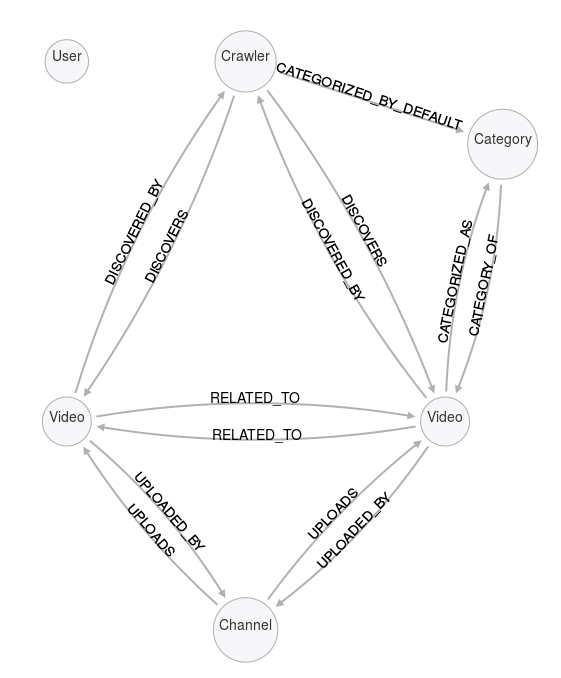
\includegraphics[scale=0.20]{desarrollo/DatabaseGraph.png}
\caption{Diseño capa de datos con nodos y aristas}
\end{figure}

Como curiosidad, \textit{Neo4j} define su propio lenguaje de consultas llamado \textit{Cypher} y proporciona una consola de administración web donde realizar consultas y visualizar los resultados en formato de grafo entre otros:
\begin{figure}[H]
\centering
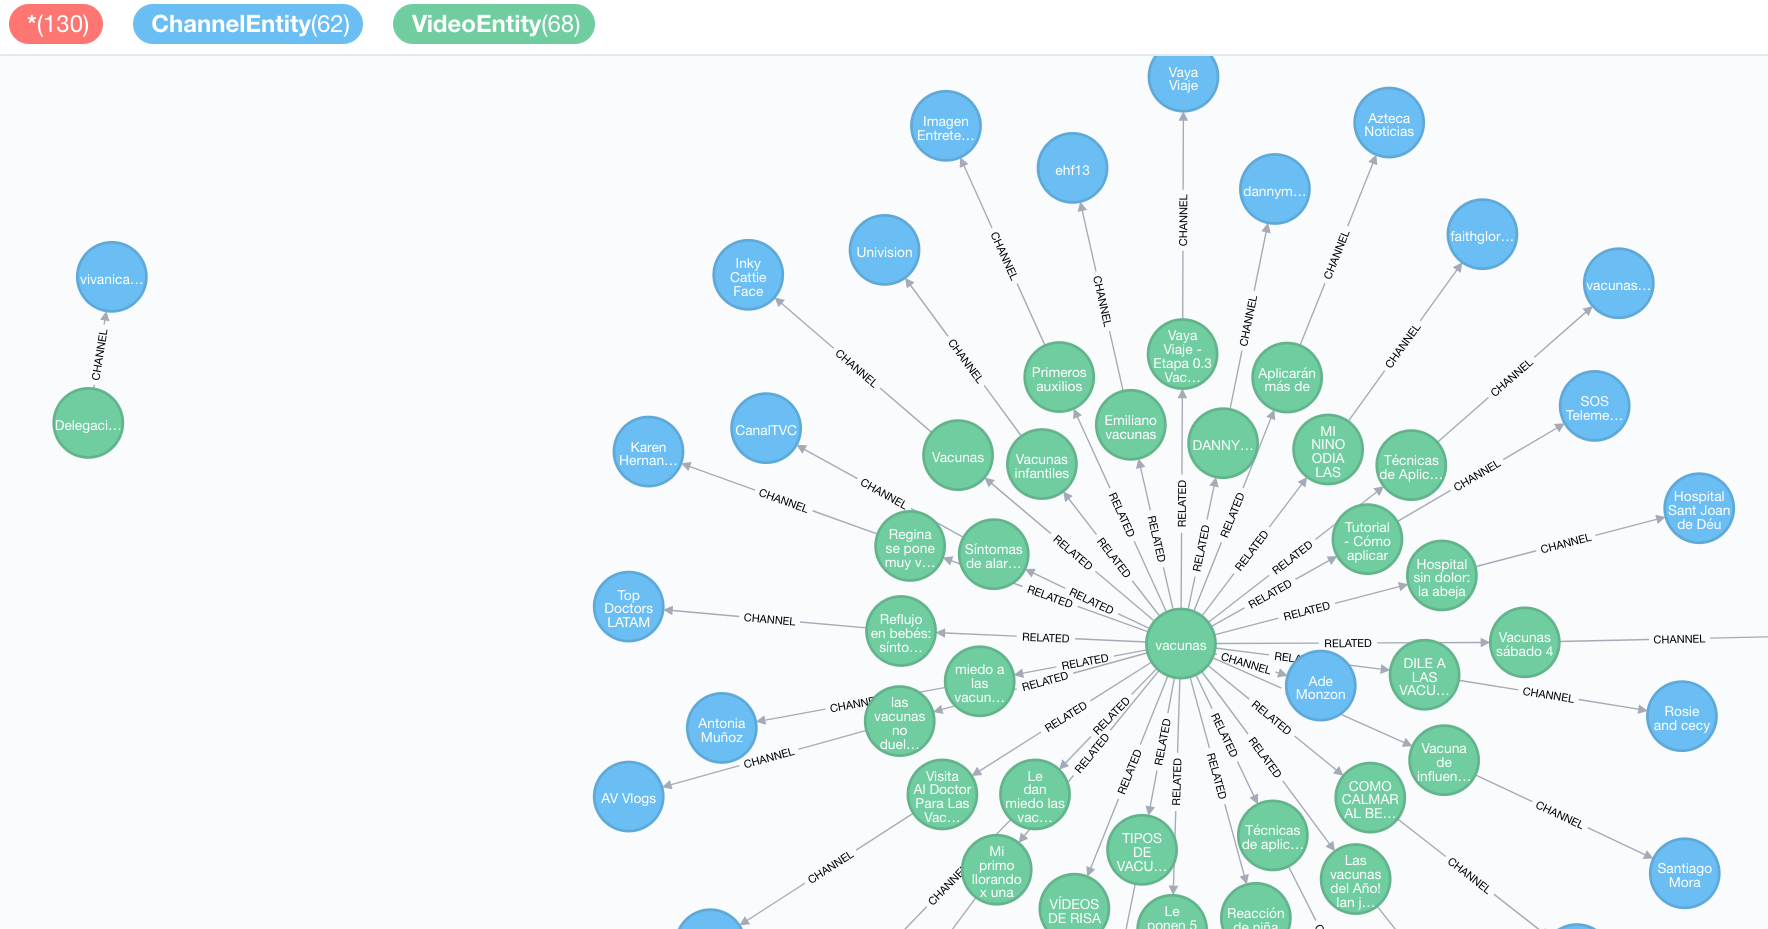
\includegraphics[scale=0.20]{desarrollo/neo4j.png}
\caption{Consola de administración \textit{Neo4j}}
\end{figure}
\pagebreak 

\subsection{Estructura de la aplicación}
Tal y como se ha avanzado anteriormente, para la creación de la estructura del proyecto en \textit{Java} se hizo uso de la herramienta \textit{Maven} (o conocido popularmente como \textit{mvn}).
\\

Con esta herramienta se creo la definición del proyecto juntamente con sus módulos utilizando los \textit{Project Object Model} (definidos mediante ficheros de configuración '\textit{pom.xml}') con los cuales es posible definir la estructura de la aplicación a construir. Ademas, \textit{Maven} nos permite gestionar las dependencias a otros módulos o librerías de terceros añadiendo versionado a nuestra aplicación.
\\

Así entonces, utilizando \textit{Maven} se definió la estructura de la aplicación separada por módulos independientes tomando como referencia la separación por paquetes realizada en el diseño de la capa de aplicación de la sección \ref{capaAplicacion}:

\begin{itemize}
\item \textbf{youtube-crawler-tool:} Modulo padre de la aplicación.
\item \textbf{youtube-crawler-tool-data:} Implementación de la capa de acceso a datos.
\item \textbf{youtube-crawler-tool-core:} Implementación de la capa de lógica de negocio.
\item \textbf{youtube-crawler-tool-api:} Implementación de la capa de presentación.
\item \textbf{youtube-crawler-tool-war:} Implementación de la capa cliente.
\end{itemize}

Gracias a esta separación por módulos, la solución implementada puede ser fácilmente ampliada para, por ejemplo, definir una capa de acceso a datos alternativa que utilice una tecnología de persistencia diferente.

\begin{figure}[H]
\centering
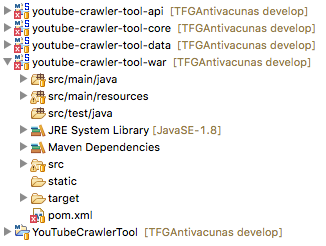
\includegraphics[scale=0.60]{desarrollo/mvn.png}
\caption{Estructura de la aplicación}
\end{figure}

A seguir se facilitan algunos extractos de los ficheros "\textit{pom.xml}" definidos para cada modulo:
\\

\noindent\textbf{youtube-crawler-tool}
\begin{lstlisting}[style=C]
...
<groupId>uoc.edu.jsanchezmend.tfg</groupId>
<artifactId>youtube-crawler-tool</artifactId>
<version>1.0.0</version>
<packaging>pom</packaging>

<parent>
  <groupId>org.springframework.boot</groupId>
  <artifactId>spring-boot-starter-parent</artifactId>
  <version>2.0.1.RELEASE</version>
</parent>
	
<!-- Modules -->
<modules>
  <module>youtube-crawler-tool-data</module>
  <module>youtube-crawler-tool-core</module>
  <module>youtube-crawler-tool-api</module>
  <module>youtube-crawler-tool-war</module>
</modules>
...
\end{lstlisting}
\medskip

\noindent\textbf{youtube-crawler-tool-data}
\begin{lstlisting}[style=C]
...
<artifactId>youtube-crawler-tool-data</artifactId>
<packaging>jar</packaging>

<parent>
  <groupId>uoc.edu.jsanchezmend.tfg</groupId>
  <artifactId>youtube-crawler-tool</artifactId>
  <version>1.0.0</version>
</parent>
    
<dependencies>
  <!-- Spring Data Neo4j -->
  <dependency>
    <groupId>org.springframework.boot</groupId>
    <artifactId>spring-boot-starter-data-neo4j</artifactId>
  </dependency>
  <!-- Json parser -->
  <dependency>
    <groupId>com.google.http-client</groupId>
    <artifactId>google-http-client-jackson2</artifactId>
    <version>1.23.0</version>
  </dependency>
</dependencies>
...
\end{lstlisting}
\medskip

\noindent\textbf{youtube-crawler-tool-core}
\begin{lstlisting}[style=C]
...
<artifactId>youtube-crawler-tool-core</artifactId>
<packaging>jar</packaging>

<parent>
  <groupId>uoc.edu.jsanchezmend.tfg</groupId>
  <artifactId>youtube-crawler-tool</artifactId>
  <version>1.0.0</version>
</parent>

<dependencies>
  <!-- YouTubeCrawlerTool data -->
  <dependency>
    <groupId>uoc.edu.jsanchezmend.tfg</groupId>
    <artifactId>youtube-crawler-tool-data</artifactId>
    <version>${parent.version}</version>
  </dependency>
  <!-- YouTube Data V3 support -->
  <dependency>
    <groupId>com.google.apis</groupId>
    <artifactId>google-api-services-youtube</artifactId>
    <version>v3-rev193-1.23.0</version>
  </dependency>
</dependencies>
\end{lstlisting}
\medskip

\noindent\textbf{youtube-crawler-tool-api}
\begin{lstlisting}[style=C]
...
<artifactId>youtube-crawler-tool-api</artifactId>
<packaging>jar</packaging>

<parent>
  <groupId>uoc.edu.jsanchezmend.tfg</groupId>
  <artifactId>youtube-crawler-tool</artifactId>
  <version>1.0.0</version>
</parent>

<dependencies>
  <!-- YouTubeCrawlerTool core -->
  <dependency>
    <groupId>uoc.edu.jsanchezmend.tfg</groupId>
    <artifactId>youtube-crawler-tool-core</artifactId>
    <version>${parent.version}</version>
  </dependency>
  <!-- Spring Boot Web -->
  <dependency>
    <groupId>org.springframework.boot</groupId>
    <artifactId>spring-boot-starter-web</artifactId>
  </dependency>
  <!-- Spring Security -->
  <dependency>
    <groupId>org.springframework.boot</groupId>
    <artifactId>spring-boot-starter-security</artifactId>
  </dependency>
</dependencies>
...
\end{lstlisting}
\medskip

\noindent\textbf{youtube-crawler-tool-war}
\begin{lstlisting}[style=C]
...
<artifactId>youtube-crawler-tool-war</artifactId>
<packaging>war</packaging>

<parent>
  <groupId>uoc.edu.jsanchezmend.tfg</groupId>
  <artifactId>youtube-crawler-tool</artifactId>
  <version>1.0.0</version>
</parent>

<dependencies>
  <!-- YouTubeCrawlerTool api -->
  <dependency>
    <groupId>uoc.edu.jsanchezmend.tfg</groupId>
    <artifactId>youtube-crawler-tool-api</artifactId>
    <version>${parent.version}</version>
  </dependency>
  <!-- Spring Boot Thymeleaf -->
  <dependency>
    <groupId>org.springframework.boot</groupId>
    <artifactId>spring-boot-starter-thymeleaf</artifactId>
  </dependency>
  <!-- optional, it brings userful tags to display spring security stuff -->
  <dependency>
    <groupId>org.thymeleaf.extras</groupId>
    <artifactId>thymeleaf-extras-springsecurity4</artifactId>
  </dependency>
  <!-- hot swapping, disable cache for template, enable live reload -->
  <dependency>
    <groupId>org.springframework.boot</groupId>
    <artifactId>spring-boot-devtools</artifactId>
    <optional>true</optional>
  </dependency>
</dependencies>
...
\end{lstlisting}
\bigskip 

\subsection{Acceso a datos}
En el modulo \textit{youtube-crawler-tool-data} se implemento la capa de acceso a datos de la aplicación. Al utilizar \textit{Neo4j} como SGBD en la capa de datos, esta capa debía de realizar y gestionar la conexión a esta base de datos i proporcionar acceso a la capa de lógica de negocio.
\\

Para su implementanción se utilizo el marco de desarrollo \textit{Spring Data} y, mas concretamente, el proyecto \textit{Spring Data Neo4j} \cite{39}. Al utilizar este marco de desarrollo, ademas de poder utilizar las características que aporta \textit{Spring Data} para dar soporte a JPA \cite{40}, como el uso de entidades para definir los objetos de dominio y uso de repositorios para la implementación de DAOs (Data Access Objects) \cite{41}, también podemos utilizar características propias que aporta el uso de \textit{Neo4j}, tales como anotaciones para la definición de grafos o soporte para el lenguaje de consultas \textit{Cypher}.
\pagebreak 

La relación de entidades (o objetos de dominio) definidos fue:
\begin{itemize}
\item \textbf{Crawler.java:} Representación en la aplicación de un proceso de recolección.
\item \textbf{Video.java:} Representación en la aplicación de un vídeo de \textit{YouTube}.
\item \textbf{Channel.java:} Representación en la aplicación de un canal de \textit{YouTube}.
\item \textbf{Category.java:} Representación en la aplicación de una categoría.
\end{itemize}

A modo ilustrativo, se añade a continuación un extracto de la entidad \textit{Video} en donde se observan algunas de las anotaciones propias del proyecto \textit{Spring Data Neo4j}:
\begin{lstlisting}[style=C]
@NodeEntity
public class Video {
  
  @Id
  protected String id;
  ...
  @Relationship(type = "UPLOADED_BY", direction = Relationship.OUTGOING)
  protected Channel channel;
	
  @Relationship(type = "RELATED_TO", direction = Relationship.OUTGOING)
  public Set<Video> related;
  ...
\end{lstlisting}
En donde la anotación \textit{@NodeEntity} identifica esta clase como un objeto de dominio o nodo en \textit{Neo4j} y la anotación \textit{@Relationship} permite definir el tipo de relación o arista entre dos nodos.
\\

Y por lo que se refiere a los repositorios para dar acceso a estas entidades en el proyecto se definieron los siguientes:
\begin{itemize}
\item \textbf{CrawlerRepository.java:} Proporciona acceso a objetos de dominio de tipo \textit{Crawler}.
\item \textbf{VideoRepository.java:} Proporciona acceso a objetos de dominio de tipo \textit{Video}.
\item \textbf{ChannelRepository.java:} Proporciona acceso a objetos de dominio de tipo \textit{Channel}.
\item \textbf{CategoryRepository.java:} Proporciona acceso a objetos de dominio de tipo \textit{Category}.
\end{itemize}

Y de igual forma que con las entidades, a continuación se proporciona un extracto del repositorio \textit{VideoRepository} para ilustrar su implementación: 
\begin{lstlisting}[style=C]
public interface VideoRepository extends Neo4jRepository<Video, String> {

  @Depth(1)
  @Query("MATCH (video:Video) WHERE video.favorite=true WITH video "
    + "MATCH v=(video)-[:UPLOADED_BY|DISCOVERED_BY|CATEGORIZED_AS]->() RETURN video, nodes(v), rels(v)")
  List<Video> findAllFavorite();
  ...		
  @Query("MATCH (v:Video) -[:DISCOVERED_BY]-> (c:Crawler) WHERE ID(c)={0} DETACH DELETE v")
  void removeByCrawlerId(Long crawlerId);
  ...
\end{lstlisting}
En el cual, al extender de \textit{Neo4jRepository} nos brinda muchas funcionalidades estandard que se suelen requerir a los objectos de acceso a datos, tales como operaciones de CRUD \cite{42}. Pero ademas, se nos permite definir nuestras propias consultas las cuales pueden estar definidas en lenguaje \textit{Cypher}.
\\

Finalmente, en esta capa también se definen los objetos planos de \textit{Java} conocidos como POJOs \cite{43}, los cuales en su gran mayoría son representaciones de las entidades definidas anteriormente y su uso esta destinado a actuar como mecanismo de comunicación (previamente serializados como JSON) entre la capa de presentación y la capa cliente.
\medskip 

\subsection{Lógica de negocio}
En el modulo \textit{youtube-crawler-tool-core} esta implementada la capa de lógica de negocio. En ella, diferentes componentes que se ofrecen como servicios a ser utilizados por la capa de presentación, acceden a los recursos definidos en la capa de acceso a datos o en servicios de terceros para implementar la lógica de negocio de la aplicación.
\medskip 

\subsubsection{Servicios}
Así entonces, en el modulo \textit{youtube-crawler-tool-core} se definen tantos servicios como componentes se definieron para la aplicación ademas de otros servicios que, se podría decir, actúan como complementos de los servicios principales. Entre los servicios complementarios se encuentran los denominados \textit{converters} que son los encargados de transformar una entidad de base de datos a su respectivo POJO y, en el caso de ser una entidad proveniente de \textit{YouTube}, también realizan la transformación de entidad de \textit{YouTube} a POJO. Ademas de los \textit{converters}, entre los servicios complementarios también encontramos el servicio \textit{YouTubeSearchService} que es el encargado de realizar las peticiones a la API de \textit{YouTube}.
\\

Aplicando esta estructuración, la aplicación respeta los principios de diseño SOLID \cite{44} al conseguirse, entre otras características,  la especialización de los servicios favoreciendo la extensibilidad y la reutilización de código. 
\\

A continuación se listan los servicios principales a los cuales se acceden desde la capa de presentación:
\begin{itemize}
\item \textbf{CrawlerService.java:} Actúa como interfaz del componente \textit{CrawlerBusiness} y en cuya implementación se encuentra la lógica de negocio necesaria para la recolección de vídeos.
\item \textbf{VideoService.java:} Actúa como interfaz del componente \textit{VideoBusiness} y en cuya implementación se encuentra la lógica de negocio relacionada con los vídeos de la aplicación.
\item \textbf{ChannelService.java:} Actúa como interfaz del componente \textit{ChannelBusiness} y en cuya implementación se encuentra la lógica de negocio relacionada con los canales de la aplicación.
\item \textbf{CategoryService.java:} Actúa como interfaz del componente \textit{CategoryBusiness} y en cuya implementación se encuentra la lógica de negocio relacionada con las categorías de la aplicación.
\item \textbf{AnalysisService.java:} Actúa como interfaz del componente \textit{AnalysisBusiness} y en cuya implementación se encuentra la lógica de negocio relacionada con la representación en grafo de vídeos y canales de la aplicación.
\end{itemize}

Y por lo que se refiere a los servicios que actúan como \textit{converters}, su listado es el siguiente:
\begin{itemize}
\item \textbf{CrawlerConverterServiceImpl.java:} Es el encargado de transformar entidades del tipo \textit{Crawler} a su respectivo POJO (\textit{CrawlerItem}) y viceversa.
\item \textbf{VideoConverterServiceImpl.java:} Es el encargado de transformar entidades del tipo \textit{Video} a su respectivo POJO (\textit{VideoItem}) y viceversa. Ademas, también realiza la trasformaciones de la entidad de \textit{Video} de \textit{YouTuve} a POJO.
\item \textbf{ChannelConverterServiceImpl.java:} Es el encargado de transformar entidades del tipo \textit{Channel} a su respectivo POJO (\textit{ChannelItem}) y viceversa. Ademas, también realiza la trasformaciones de la entidad de \textit{Channel} de \textit{YouTuve} a POJO.
\item \textbf{CategoryConverterServiceImpl.java:} Es el encargado de transformar entidades del tipo \textit{Category} a su respectivo POJO (\textit{CategoryItem}) y viceversa.
\end{itemize}

Para conectar todos estos servicios entre si y habilitarlos en la capa de presentación, en el proyecto se hace un uso extensivo del patrón de inyección de independencias proporcionado por el marco de desarrollo \textit{Spring Core}, el cual se encarga de instanciar objetos y inyectarlos como dependencias allí donde  sean necesarias. De esta forma, se consigue un alto desacoplamiento entre los distintos componentes lo cual facilita el mantenimiento y la reusablilidad del código.
\\

Para aplicar el patrón de inyección de independencias se ha utilizado el mecanismo de anotaciones habilitado por \textit{Spring Core}. En el cual, para definir una nueva instancia a injectar se ha utilizado la anotación \textit{@Service} y para inyectar una dependencia la anotación \textit{@Autowired} tal y como se demuestra en el siguiente extracto de la implementación del servicio \textit{VideoService}.
\begin{lstlisting}[style=C]
@Service("videoService")
public class VideoServiceImpl implements VideoService {
  
  @Autowired
  private VideoRepository videoRepository;
  ...
  @Autowired
  @Qualifier("videoConverterService")
  private YouTubeConverterService<com.google.api.services.youtube.model.Video, Video, VideoItem> videoConverterService;
  ...
\end{lstlisting}	

\medskip 

\subsubsection{Crawler de YouTube}
Una de las funcionalidades mas destacadas que se implementaron en la capa de lógica de negocio fue el proceso recolector (\textit{crawler} en ingles) de vídeos de \textit{YouTube}. En esta sección se detallan las características mas relevantes de dicha implementación.
\\

Antes de nada, para poder desarrollar un proceso de recolección había que definir el modo en el cual la aplicación realizaría peticiones a la \textit{YouTube Data API}. Para tales efectos, se definió en la aplicación el servicio \textit{\textbf{YouTubeSearchService}} el cual tiene la responsabilidad de realizar dichas peticiones.
\\

Para realizar las peticiones a la API de \textit{YouTube} se decidió hacer uso de la librería \textit{Java} cliente de la \textit{YouTube Data API} definida por \textit{Google} \cite{45}. Gracias a esta librería podíamos extraernos de realizar y gestionar las peticiones HTTP a los servicios requeridos de la API de \textit{YouTube} ya que las comunicaciones con este servicio extorno se podían realizar como si de otro servicio de la aplicación se tratase.
\\

Para importar en el proyecto la librería cliente de la \textit{YouTube Data API} fue necesario añadir la siguiente dependencia en el fichero \textit{pom.xml} del modulo \textit{youtube-crawler-tool-core} de la siguiente forma:
\begin{lstlisting}[style=C]
  ...
  <!-- YouTube Data V3 support -->
  <dependency>
    <groupId>com.google.apis</groupId>
    <artifactId>google-api-services-youtube</artifactId>
    <version>v3-rev193-1.23.0</version>
  </dependency>
  ...
\end{lstlisting}	

Y para inicializar el servicio de \textit{YouTube} que realizaría nuestras peticiones a la API de \textit{YouTube}, se añadió la siguiente instancia al contexto de \textit{Spring} mediante una clase de configuración:
\begin{lstlisting}[style=C]
@Configuration
public class YouTubeConfiguration {
  protected static final String YOUTUBE_APPLICATION_NAME="youtube-crawler-tool-app";
  
  @Bean
  public YouTube youTube() {
    // This object is used to make YouTube Data API requests.
    final YouTube youtube = new YouTube.Builder(new NetHttpTransport(), new JacksonFactory(),
      (request) -> {}).setApplicationName(YOUTUBE_APPLICATION_NAME).build();
    return youtube;
  }
}
\end{lstlisting}	
\pagebreak 

Ahora, cada vez que se requiriera realizar una petición a la API de \textit{YouTube}, se podía realizar utilizando el servició definido indicando en cada petición la \textit{Google API Key} obtenida al configurar el entorno de desarrollo en el apartado \ref{entorno} y que esta configurada en la aplicación mediante la propiedad \textit{'ytct.youtube.api.key'}. 
\\

La relación completa de los métodos definidos en el servicio \textit{YouTubeSearchService} es la siguiente:
\begin{itemize}
\item \textbf{searchVideos():} Realiza la petición al servicio \textit{'Search: list'} de la API de \textit{YouTube} para realizar una búsqueda textual y obtener un listado de identificadores de vídeos como respuesta.
\item \textbf{searchRelatedVideos():} Realiza la petición al servicio \textit{'Search: list'} de la API de \textit{YouTube} para realizar una búsqueda por vídeo relacionado y obtener un listado de identificadores de vídeos como respuesta.
\item \textbf{findVideos():} Realiza la petición al servicio \textit{'Videos: list'} de la API de \textit{YouTube} para recuperar el contenido de los vídeos dado un listado de identificadores de vídeos.
\item \textbf{findChannel():} Realiza la petición al servicio \textit{'Channels: list'} de la API de \textit{YouTube} para recuperar el contenido de un canal dado un identificador de canal.
\end{itemize}

Habiendo resuelto el modo en el que se realizarían las peticiones a la API de \textit{YouTube} mediante el servicio \textit{YouTubeSearchService}, ahora era el momento de definir el proceso de recolección propiamente dicho. Para tales efectos se diseño el servicio \textit{\textbf{CrawlerService}} el cual tiene la responsabilidad de realizar y gestionar los procesos de recolección.
\\

A continuación se proporciona un pseudocódigo resumido a modo ilustrativo del proceso de recolección implementado en el servicio \textit{CrawlerService}:
\begin{lstlisting}[style=C]
Funcion doCrawler(crawler)
  crawler.status <- RUNNING;
  Hacer
    busqueda <- youTubeSearchService.searchVideos(crawler);
    
    videos <- youTubeSearchService.findVideos(busqueda.videoIds);
    Para i <- 0 Hasta i = videos.size() Hacer
      Si videoRepository.findBy(video.id) = null Entonces
        videoRepository.save(video);
        
        Si channelRepository.findBy(video.channelId) = null Entonces
          channel <- youTubeSearchService.findChannel(video.channelId);
          channelRepository.save(channel);
        Fin Si
      Fin Si
      
      Si crawler.nivelRelacionado > 0) Entonces
        nuevoCrawler <- new Crawler();
        nuevoCrawler.videoRelacionado <- video.id;
        nuevoCrawler.nivelRelacionado <- crawler.nivelRelacionado -1;
        nuevoCrawler.videosRelacionados <- crawler.videosRelacionados;
        doCrawler(nuevoCrawler);
      Fin Si
      
      i <- i+1;
    Fin Para
    
    Si busqueda.siguientePagina = null Entonces
      crawler.status <- FINISHED;
    Si no Entonces
      crawler.pagina <- busqueda.siguientePagina;
    Fin Si
    
  Mientras crawler.status = RUNNING
  
Fin Funcion
\end{lstlisting}	


Uno de los requerimientos del proyecto era poder realizar varios procesos de recolección de forma simultanea y controlar su ejecución. Por lo tanto, los procesos de recolección debían de ejecutarse en hilos de ejecución (o \textit{Threads} en ingles) distintos al hilo principal de la aplicación para, de este modo, no bloquear el funcionamiento de la herramienta y permitir la ejecución asíncrona en paralelo de varios procesos de recolección.
\\

Para habilitar la ejecución asíncrona de varios procesos de recolección, de nuevo se utilizaron las capacidades ofrecidas por el marco de trabajo \textit{Spring} para la creación y gestión de los hilos de ejecución. Concretamente, para su configuración fue necesario instanciar un \textit{TaskExecutor} mediante la clase de configuración \textit{AsyncExecutorConfiguration} y anotar posteriormente con la anotación \textit{@Async} el método deseado. De esta forma, cada vez que se ejecutara el método anotado con la anotación \textit{@Async}, el \textit{TaskExecutor} configurado crearía y gestionaría un nuevo hilo de ejecución para su procesado.
\newpage 

Así entonces, en nuestro caso el método que iniciaba la ejecución de un proceso de recolección tenia que ser anotado con la anotación \textit{@Async} de la siguiente forma:
\begin{lstlisting}[style=C]
  @Async
  @Override
  public CompletableFuture<CrawlerItem> executeCrawler(Long crawlerId) {
\end{lstlisting}	

Finalmente, el uso de varios hilos de ejecución puede producir errores de concurrencia si mas de un hilo intenta acceder al mismo recurso al mismo tiempo. Para evitar este tipo de problemas, en el código se protegieron los recursos que eran susceptibles de ser accedidos por varios hilos de ejecución al mismo tiempo con la sentencia \textit{synchronized}. De esta forma, cuando un hilo de ejecución entra dentro de un bloque con la sentencia \textit{synchronized}, evita que cualquier otro hilo acceda también dentro de dicho bloque o a los recursos del mismo.
\\

Por ejemplo, durante la ejecución de un proceso de recolección el usuario puede cambiar su estado para detenerlo. Para asegurar que ningún proceso esta cambiando el estado del mismo proceso de recolección al mismo tiempo y evitar problemas de consistencia, se utiliza la sentencia \textit{synchronized} de la siguiente forma:
\begin{lstlisting}[style=C]
  synchronized (this) {
    final Crawler crawler = this.crawlerRepository.findById(id).orElse(null);
    ...
    crawler.setStatusByEnum(newStatus);
    this.crawlerRepository.save(crawler);
    ...
  }
\end{lstlisting}	

\medskip

\subsection{Presentación}
En el modulo \textit{youtube-crawler-tool-api} es donde se implemento el controlador de solicitudes de recursos para habilitar la API REST de la aplicación y en el modulo \textit{youtube-crawler-tool-war} el controlador de solicitudes de navegador y la capa cliente de la aplicación web. A continuación en los siguientes apartados se detallan las características mas relevantes de su implementación.
\medskip 

\subsubsection{Solicitudes de recursos}
Para habilitar la API REST de la aplicación definida en el apartado \ref{rest}, en el modulo \textit{youtube-crawler-tool-api} se hace uso del marco de desarrollo \textit{Spring MVC} \cite{46}. Gracias al cual, fue posible definir la API REST, los recursos disponibles y sus métodos mediante el uso de anotaciones en cada una de las clases de tipo \textit{controller} que fueron definidas para cada componente.
\\

Es en estas clases tipo \textit{controller} es donde se realizan peticiones a los servicios habilitados en la capa de lógica de negocio para responder a las peticiones de recursos realizadas por los usuarios los cuales son devueltos en formato JSON. El listado completo de \textit{controllers} definidos es el siguiente:

\begin{itemize}
\item \textbf{CrawlerController.java:} Gestiona peticiones de recursos del tipo procesos de recolección. Responde a peticiones realizadas a la ruta \textit{'/api/crawlers'}.
\item \textbf{VideoController.java:} Gestiona peticiones de recursos del tipo vídeos. Responde a peticiones realizadas a la ruta \textit{'/api/videos'}.
\item \textbf{ChannelController.java:} Gestiona peticiones de recursos del tipo canales. Responde a peticiones realizadas a la ruta \textit{'/api/channels'}.
\item \textbf{CategoryController.java:} Gestiona peticiones de recursos del tipo categorías. Responde a peticiones realizadas a la ruta \textit{'/api/categories'}.
\item \textbf{AnalysisController.java:} Gestiona peticiones de recursos del tipo grafos. Responde a peticiones realizadas a la ruta \textit{'/api/graphs'}.
\end{itemize}

A modo de ejemplo, se incluye a continuación un extracto del controlador \textit{VideoController.java}:
\begin{lstlisting}[style=C]
@Controller
@RequestMapping("/api/videos")
public class VideoController {
  
  @Autowired
  private VideoService videoService;
  
  @ResponseBody
  @RequestMapping(value = "/favorites", method = RequestMethod.GET)
  public List<VideoItem> listFavoritesVideos() {
    return this.videoService.listFavoritesVideos();
  }
  ...
\end{lstlisting}	


La API REST habilitada mediante estos controladores es consumida por la interfaz web implementada en la capa cliente. En ella, las diferentes vistas de la aplicación realizan peticiones HTTP para acceder a los recursos necesarios. Dichas peticiones se realizan de forma asíncrona utilizando la librería de \textit{JavaScript} \textit{JQuery} y, mas concretamente, haciendo uso de la función \textit{ajax()} \cite{47}.
\\

Para evitar la repetición de código en la capa cliente, se definió una librería \textit{JavaScript} llamada  \textit{youtube-crawler-tool.js} en la cual se implementan de forma genérica las llamadas \textit{ajax}. Por ejemplo, el código \textit{JavaScript} para realizar una petición \textit{ajax} de tipo GET se define de la siguiente forma:
\begin{lstlisting}[style=C]
var doGet = function (requestUrl, callback) {
  console.log("doGet for url: " + requestUrl);
  $.ajax({ 
    url: requestUrl, 
    method: 'GET', 
    success: callback
  });
}
\end{lstlisting}	

En donde, de querer obtener el listado de vídeos favoritos realizaríamos una petición a la API REST de tipo GET de la siguiente forma:
\begin{lstlisting}[style=C]
doGet("/api/videos/favorites", function (favorites) {
  ...
});
\end{lstlisting}	

\medskip 

\subsubsection{Solicitudes de navegador}
En el modulo \textit{youtube-crawler-tool-war} es donde se encuentra implementada la capa cliente de la aplicación y el controlador de solicitudes de navegador.
\\

Dicho controlador es implementado en la clase \textit{YouTubeCrawlerToolController.java} en donde, gracias al uso de \textit{Spring MVC}, se definen las peticiones a las diferentes vistas de la aplicación. A diferencia de los \textit{controllers} definidos para las solicitudes de recursos, en el controlador de solicitudes de navegador como respuestas se devuelven redirecciones a las vistas definidas para cada caso.
\\

A modo de ejemplo, se incluye a continuación un extracto de la clase \textit{YouTubeCrawlerToolController.java} en el cual se gestiona la petición a la vista en detalle de un vídeo en concreto:
\begin{lstlisting}[style=C]
@Controller
@RequestMapping("/")
public class YouTubeCrawlerToolController {
  ...
  private static final String VIDEOS_VIEW = "videosView.html";
  ...
  @RequestMapping(value="videos/{id}")
  public String getVideoView(Model model, @PathVariable(value = "id", required = true) String id) {
    model.addAttribute("activeMenuOption", VIDEOS_VIEW);
    model.addAttribute("videoId", id);
    return VIDEO_VIEW;
  }
  ...
\end{lstlisting}	

Para la construcción de las vistas html de la aplicación, se utilizo el motor de plantillas para Java \textit{Thymeleaf} \cite{48}, el cual, es el recomendado actualmente por la plataforma \textit{Spring}. Con  \textit{Thymeleaf} es posible definir plantillas HTML permitiendo inyectar código servidor de una forma muy natural ademas de ofrecer integración con \textit{Spring}. Utilizando esta tecnología fue posible implementar las vistas definidas en el apartado \ref{capaCliente}.
\\

Para no partir de cero en el desarrollo de dichas vistas, como punto de partida se decidió buscar una plantilla html que se adaptara fácilmente a las funcionalidades diseñadas para la aplicación y que tuviera una licencia libre de uso. La plantilla escogida para tales efectos fue \textit{SB Admin 2} \cite{49}. 
\medskip 

\subsubsection{Seguridad de vistas y recursos}
Uno de los requerimientos de la aplicación era la definición de dos tipos de usuarios distintos:
\begin{itemize}
\item \textbf{Usuario anónimo:} Solo se le permite realizar acciones de lectura en la aplicación y generar grafos.
\item \textbf{Usuario identificado:} Se le permite realizar cualquier acción en la aplicación.
\end{itemize}

Este requerimiento conllevaba proveer a la aplicación de la funcionalidad necesaria para la identificación de usuarios mediante inicio de sesión y añadir una capa de seguridad para proteger los recursos y vistas que no fueran de dominio publico. Para conseguirlo, la aplicación hizo uso del marco de trabajo \textit{Spring Security} \cite{50}.
\\

Al añadir \textit{Spring Security} al proyecto, por defecto se provee a la aplicación de la funcionalidad necesaria para identificar y crear sesiones de usuario en la aplicación realizando peticiones de tipo POST \textit{/login} tal y como se realiza en la vista \textit{loginView.html}. Para probar dicha funcionalidad, en la clase de configuración \textit{YouTubeCrawlerToolSecurityConfiguration.java}, al levantarse la aplicación se añade al contexto de \textit{Spring} un usuario de prueba cuyo nombre y contraseña se definen en las propiedades \textit{ytct.security.default.username} y \textit{ytct.security.default.password}.
\\

Es también en la clase de configuración \textit{YouTubeCrawlerToolSecurityConfiguration.java} en donde se protegen los recursos ofrecidos por la API REST de la aplicación. En este caso, para cumplir con los requerimientos de la aplicación, teníamos que proteger todas las peticiones a recursos que no fueran de tipo GET para asegurarnos que el usuario que las realiza es un usuario identificado. Dicha configuración se facilita a continuación:
\begin{lstlisting}[style=C]
  @Override
  protected void configure(HttpSecurity http) throws Exception {
    http
      .csrf().disable()
        .authorizeRequests()
          // Crawler component security
          .antMatchers(HttpMethod.POST,	"/api/crawlers").authenticated()
          .antMatchers(HttpMethod.PUT,	"/api/crawlers").authenticated()
          .antMatchers(HttpMethod.DELETE,	"/api/crawlers").authenticated()
          // Video component security
          .antMatchers(HttpMethod.PUT,	"/api/videos").authenticated()
          .antMatchers(HttpMethod.DELETE,	"/api/videos").authenticated()
          // Channel component security
          .antMatchers(HttpMethod.DELETE,	"/api/channels").authenticated()
          // Category component security
          .antMatchers(HttpMethod.POST,	"/api/categories").authenticated()
          .antMatchers(HttpMethod.PUT,	"/api/categories").authenticated()
          .antMatchers(HttpMethod.DELETE,	"/api/categories").authenticated()
          // Allow any other request
          .anyRequest().permitAll()
          .and()
          .formLogin()
            .loginPage("/login")
            .permitAll()
            .and()
          .logout()
            .logoutSuccessUrl("/")
            .permitAll();
  }
\end{lstlisting}

Finalmente, para proteger las vistas a las cuales es necesario estar identificado para poder acceder (por ejemplo, en el caso de la vista de vídeos favoritos), gracias a la integración de \textit{Thymeleaf} con \textit{Spring} es posible definir enlaces en las vistas que solo serán renderizados en el caso de cumplirse unos requerimientos de seguridad en concreto. Por ejemplo, en el caso del enlace para acceder a la vista de vídeos favoritos, mediante la etiqueta \textit{sec:authorize} es posible definir que el código html en donde esta definido esta etiqueta solo se renderice en caso que el usuario este identificado:
\begin{lstlisting}[style=C]
<li class="dropdown" sec:authorize="isAuthenticated()">
  <a class="dropdown-toggle" th:href="@{/videos/favorites}" id="favoriteVideosView">
    Favorites <i class="fa fa-star fa-fw"></i>
  </a>
</li>
\end{lstlisting}
\medskip 

\subsubsection{Visualización de vídeos en grafo}
En la capa cliente de la aplicación, en las vistas html se utilizan varias librerías \textit{JavaScript} que aportan funcionalidades de presentación mejoradas a la interfaz gráfica. La mas destacada de ellas es la librería \textit{Cytoscape.js} \cite{51} que es utilizada para la visualización del grafos en la vista de análisis.
\\

Dicha librería consume una fuente de datos en formato JSON en donde se especifican los nodos y las aristas para la construcción del grafo. Gracias a su facilidad de uso y a las posibilidades de personalización que hicieron posible cumplir los requisitos de visualización de la clienta definidos en el apartado \ref{propuestaGrafo}, se eliguio su uso en la aplicación por encima de otras alternativas como \textit{D3.js} \cite{52} o \textit{Sigma.js} \cite{53}.
\\

Para obtener los nodos y las aristas en el formato JSON requerido por la librería, la interfaz de usuario realiza una petición asíncrona al recurso \textit{POST api/graphs} el cual devuelve los vídeos y canales que hayan sido recolectados previamente por el sistema y que sean resultados de unos criterios de búsqueda introducidos por el usuario.
\\

A continuación se facilita un ejemplo de la respuesta JSON obtenida por el recurso \textit{POST api/graphs} y que cumple con el formato requerido por la librería \textit{Cytoscape.js}:
\begin{lstlisting}[style=C]
{
  "elements": {
    "nodes": [
      {
        "data": {
          "id": "v-haqi4xvjvKo",
          "resourceId": "haqi4xvjvKo",
          "typeCode": "v",
          "shape": "ellipse",
          "color": "#dd1313",
          "size": 25,
          "video": {
            //campos propios del objecto video
          }
        }
      },
      ...
    ],
    "edges": [
      {
        "data": {
          "source": "v-L0jQz6jqQS0",
          "target": "v-5d667Bb_iYA",
          "outgoing": "L0jQz6jqQS0",
          "incoming": "5d667Bb_iYA",
          "outgoingType": "v",
          "incomingType": "v"
        }
      },
      ...
    ]
  }
}
\end{lstlisting}

Una vez obtenida la respuesta, en la aplicación se genera un nuevo grafo inicializando \textit{Cytoscape.js} con los elementos obtenidos de la siguiente forma:
\begin{lstlisting}[style=C]
function initCytoscape(elements) {
  cy = cytoscape({
    container: document.getElementById('cy'),
    style: cytoscape.stylesheet()
      .selector('node')
        .css({
          'shape': 'data(shape)',
          'background-color': 'data(color)',
          'width': 'mapData(size, 0, 100, 10, 60)',
          'height': 'mapData(size, 0, 100, 10, 60)'
        })
      .selector('edge')
        .css({
          'curve-style': 'haystack' // fast edges!
        }),
      layout: {
        name: 'cose',
        animate: false,
        idealEdgeLength: 100,
        nodeOverlap: 20,
        refresh: 20,
        fit: true,
        padding: 30,
        randomize: false,
        componentSpacing: 100,
        nodeRepulsion: 400000,
        edgeElasticity: 100,
        nestingFactor: 5,
        gravity: 80,
        numIter: 20,
        initialTemp: 200,
        coolingFactor: 0.95,
        minTemp: 1.0
      },
      elements: elements
   });
   
   cy.nodes().forEach(function(node){
     nodeJson = node.json();
     cy.getElementById(node.id()).qtip({
       content: generateNodeContent(nodeJson.data),
       position: {
         my: 'top center',
         at: 'bottom center'
       },
       style: {
         classes: 'qtip-bootstrap',
         tip: {
           width: 16,
           height: 8
         }
       }
     });
   });
   ...
 };
\end{lstlisting}
\medskip 

\subsection{Definición y ejecución de pruebas}
Durante el desarrollo de la aplicación y a medida que se iba finalizando la implementación de los distintos componentes, se fueron definiendo y ejecutando pruebas de integración para probar la funcionalidad desarrollada.
\\

Las pruebas a realizar se definieron según los casos de uso documentados en la sección \ref{casosDeUso} asignando un código de identificación para cada uno de ellos. Ademas, al agrupar las pruebas a realizar por componentes nos permitió evaluar la calidad de cada componente por separado tan pronto estaba disponible.
\\

En el apartado anexo \ref{pruevasIntegracion} se facilita el resultado completo de las pruebas de integración realizadas.
\medskip 

\subsection{Pruebas de concepto}\label{pocs}
Tal y como se ha comentado en anteriores apartados, en el desarrollo de la aplicación se realizaron varias pruebas de concepto para poner a prueba distintas soluciones y estudiar la viabilidad se ser incorporadas en el sistema.
\\

En esta apartado se resume brevemente cada una de ellas junto con su finalidad y los resultados obtenidos:
\\

\noindent\textbf{POCTwitterCrawler}\\
\textbf{Descripción:} Prueba de concepto desarrollada para probar la integración con la API de \textit{Twitter} y guardar los contenidos recolectados en \textit{MongoDB}.\\
\textbf{Resultados:} Aunque la prueba resulto satisfactoria y fue posible obtener mensajes de \textit{Twitter} y guardarlos en \textit{MongoDB}, debido a la posterior elección de \textit{YouTube} como red social a utilizar y a \textit{Neo4j} como SGBD, no se pudo aprovechar el conocimiento adquirido para la implementación final.\\
\textbf{Enlace:} \url{https://github.com/jsanchezmend/TFGAntivacunas/tree/master/POCTwitterCrawler}.
\\

\noindent\textbf{POCYouTubeCrawler}\\
\textbf{Descripción:} Prueba de concepto desarrollada para probar la integración con la API de \textit{YouTube} y guardar los contenidos recolectados en \textit{MongoDB}. Posteriormente también se añadio la visualización en grafo utilizando librería JavaScript '\textit{Cytoscape.js}'.\\
\textbf{Resultados:} La prueba resulto satisfactoria y fue posible obtener mensajes de \textit{YouTube} y guardarlos en \textit{MongoDB} ademas de su visualización en formato de grafo. De esta prueba de concepto en la implementación de la aplicación se aprovecho el conocimiento adquirido a la hora de utilizar la API de\textit{YouTube} y de mostrar los videos en formato de grafo.\\
\textbf{Enlace:} \url{https://github.com/jsanchezmend/TFGAntivacunas/tree/master/POCYouTubeCrawler}.
\\

\noindent\textbf{POCYouTubeCrawlerNeo4j}\\
\textbf{Descripción:} Prueba de concepto desarrollada para probar la persistencia de contenidos recolectados en \textit{Neo4j}.\\
\textbf{Resultados:} La prueba resulto satisfactoria y fue posible guardar los contenidos recolectados en \textit{Neo4j}. El conocimiento adquirido a la hora de implementar el acceso a los datos utilizando \textit{Neo4j} como capa de datos fue utilizado en la implementación final de la aplicación.\\
\textbf{Enlace:} \url{https://github.com/jsanchezmend/TFGAntivacunas/tree/master/POCYouTubeCrawlerNeo4j}.
\\

\newpage 


\section{Implementación y puesta en funcionamiento}
\bigskip 

\subsection{Servidor de explotación}
Para dar acceso a la clienta y \textit{stakeholders}, se habilito un servidor de explotación desde donde el cual poder acceder a la aplicación.
\\

Fue con la aplicación instalada en este servidor donde la clienta pudo realizar el estudio sobre el movimiento antivacunas en la red social \textit{YouTube} recolectando vídeos y analizando sus relaciones. La aplicación instalada en este servidor fue actualizándose a medida que se avanzaba en el desarrollo.
\\

Para realizar la instalación de la aplicación se realizo el procedimiento detallado en el manual de instalación descrito en el apartado \ref{Manual} del anexo a este documento. También en el anexo en la sección \ref{IlustracionApp}, se encuentran ilustraciones de la puesta en funcionamiento de la aplicación con imágenes de la ultima versión instalada.
\\

Inicialmente, para tales efectos se habilito una aplicación Web en el servicio \textit{Microsoft Azure} con el dominio: \url{http://youtubecrawlertoolwebapp.azurewebsites.net}. Pero debido a los recursos necesarios para la instalación de Neo4j y al escaso presupuesto que \textit{Microsoft Azure} ofrece a las cuentas de estudiante, rápidamente este servició quedo bloqueado por falta de presupuesto disponible.
\\

\medskip 

\subsection{Formación y sensibilización}
En toda aplicación, ya sea de escritorio, móvil o web, para el usuario existe una primera fase de aprendizaje o de sensibilización que es mas o menos prolongada en medida de lo usable y bien diseñada que este una aplicación.
\\

\textit{YouTubeCrawlerTool} no es una excepción y, aunque la aplicación goza de una alta usabilidad bajo el criterio de la propia clienta, se han llevado a cabo sesiones de formación para acelerar este proceso.
\\

Dichas sesiones se realizaron de forma online en las cuales asistieron la clienta y los \textit{stakeholders} de la aplicación, llegando a enregistrarse una de las sesiones en \textit{YouTube}: \url{https://youtu.be/ETWtbywxOmI}.
\\

Gracias a estas sesiones, ademas de sensibilizar a los futuros usuarios de la aplicación, sirvieron para recoger sugerencias y mejoras con las cuales se llevaron a cabo posteriores refinamientos de la aplicación, como por ejemplo la adicción de la funcionalidad de favoritos o una visualización diferente para los listados de vídeos.

\medskip 

\subsection{Funcionalidades no implementadas}
De las funcionalidades diseñadas y recogidas como requisitos de la aplicación en forma de casos de uso en la sección \ref{casosDeUso}, las únicas que no han sido finalmente implementadas en la aplicación son las relativas a la habilitación de información estadística sobre el estado de la aplicación y la categorización de vídeos realizada. Concretamente los casos de uso no implementados han sido:

\begin{itemize}
\item \textbf{UC\_2:} View all crawlers statistics.
\item \textbf{UC\_8:} View crawler process statistics.
\item \textbf{UC\_16:} View all channels statistics.
\item \textbf{UC\_19:} View channel statistics.
\end{itemize}

Las razones por las que estos casos de uso no se llegaron a implementar son debido a falta de tiempo para su desarrollo y la priorización de otras funcionalidades en detrimento de estas. En la sección \ref{sec:seguiminetoPlanificacion} se proporcionan más detalles sobre estas decisiones.
\newpage 


\section{Conclusiones}
\bigskip 

\subsection{Conclusiones del trabajo}
En la realización de este trabajo ademas de darme la oportunidad de poner a prueba los conocimientos adquiridos durante el grado en ingeniería informática, me ha permitido experimentar como es el proceso de desarrollo de software en contacto directo con los usuarios finales y, en este caso, con la clienta de la solución.
\\

Gracias a esta circunstancia, he podido obtener lecciones muy valiosas que creo que me serán de utilidad en el futuro. Ya que, al tener contacto con la usuaria final de la aplicación durante todo el desarrollo de la misma, he podido aprender de su perspectiva y no centrarme únicamente en el desarrollo de la solución. Una de las conclusiones mas valiosas que he obtenido, es que en un proyecto de software siempre se pueden producir cambios (sobretodo en etapas finales), y debido a ello, hay que estar siempre atento y prevenirlos para minimizar sus riesgos siempre que sea posible.
\\

Como resultado de esta colaboración y la metodología utilizada, la aplicación obtenida ademas de cumplir los objetivos marcados al inicio del proyecto, a conseguido cumplir con las expectativas de la clienta permitiendo iniciar el estudio del movimiento antivacuna en la red social \textit{YouTube}. En palabras de la propia Johanna Milena Rodríguez Vera clienta de la aplicación:
\\

\textit{La herramienta tiene una interfaz visual que le facilita al usuario realizar las búsquedas y los filtros que son necesarios para encontrar la información que necesita.}

\textit{Por las características que tiene al API de YouTube los resultados que se obtienen se encuentran  dependiendo de la localización de quien realiza la búsqueda, siendo diferentes los vídeos que se proponen aunque tengan los mismos términos de búsqueda y filtrado. Este punto se puede convertir en un aspecto interesante a evaluar en el futuro por parte del investigador.}

\textit{Debido a como YouTube relaciona sus contenidos, los vídeos que se muestran como resultado en muchas ocasiones no tienen relación alguna con el término utilizado. Con lo cual hace necesario un trabajo manual de filtrado de la información por parte del investigador para categorizar correctamente los vídeos que se obtienen como resultado.}

\textit{La funcionalidad de grafos con la selección de múltiples variables, permite en éste escenario la obtención de grafos con diferente información que puede permitir de manera posterior su análisis de acuerdo a las características del estudio.}
\\

Ademas de lo expuesto hasta el momento, personalmente la realización de este proyecto me ha permitido desarrollar una aplicación de principio a fin, pasando des de la etapa de definición y diseño de la solución al desarrollo de la capa de datos, de aplicación y de la interfaz de usuario, obteniendo una visión global sobre el significado de desarrollar software. Por otro lado, he aprendido nuevas tecnologías tales como el uso de bases de datos NoSQL orientadas a grafos, que considero muy interesantes y con las cuales me gustaría trabajar en el futuro.
\\

Así entonces, por los puntos destacados anteriormente y por el grado de satisfacción conseguido por la usuaria, considero que la realización del proyecto ha sido un éxito.
\medskip 

\subsection{Grado de cumplimiento de los objetivos}
Aunque algunas de las funcionalidades diseñadas inicialmente para el proyecto no se han llegado a implementar (tales como la incorporación de datos estadísticos sobre la categorización de los contenidos), se han podido lograr todos los objetivos planteados inicialmente en el apartado \ref{objectivos}.
\\

A continuación se facilita la relación de objetivos definidos y su grado de cumplimiento al termino del desarrollo del proyecto:

\begin{itemize}
\item \textbf{Investigar que funcionalidades aportan las API públicas ofrecidas por \textit{YouTube} y analizar como se pueden utilizar para la obtención de la información requerida}: Se ha analizado la API de \textit{YouTube} en la sección \ref{youTubeDataAPI} y se ha estudiado conjuntamente con la clienta que información va a ser recolectada por la aplicación. Este objetivo se realizo durante la primera fase de desarrollo.
\item \textbf{Determinar como almacenar y acceder de forma eficiente a la gran cantidad de información que se obtendrá}: Se ha tomado la decisión de utilizar una base de datos NoSQL enfocada a grafos (\textit{Neo4j}) para poder acceder a la información de forma eficiente. Se ha diseñado un diagrama UML para representar el esquema invariante de la información y se ha adaptado al concepto de nodos y relaciones de las base de datos de grafos. Se realizo una prueba de concepto para estudiar la viabilidad de utilizar \textit{Neo4j} como base de datos en el proyecto con resultado favorable. La prueba de concepto realizada fue utilizada como base para la implementación de la aplicación durante la segunda fase de desarrollo. Este objetivo se considera realizado.
\newpage 
\item \textbf{Permitir la recolección de información según criterios de búsqueda proporcionados por el usuario final}: Conjuntamente con el cliente se han determinado los criterios de búsqueda a utilizar. Se ha desarrollado una prueba de concepto en la cual ha sido posible recolectar información de vídeos y canales utilizando la API de \textit{YouTube}. La prueba de concepto realizada fue utilizada como base para la implementación de la aplicación durante la segunda fase de desarrollo. Este objetivo se considera realizado.
\item \textbf{Habilitar la gestión, visualización y exportación de datos obtenidos en distintos procesos de extracción para su posterior análisis en herramientas especializadas}: Se ha diseñado una interfaz de usuario para proporcionar estas funcionalidades y se ha diseñado la arquitectura de la aplicación para hacerlas viables. En la segunda fase de desarrollo se ha adoptado y implementado la arquitectura propuesta en la primera fase de desarrollo y la interfaz de usuario necesarias para habilitar estas funcionalidades al usuario final. Este objetivo se considera realizado.
\item \textbf{Ofrecer herramientas de visualización para el análisis y comprensión de los datos obtenidos}: Se ha decidido el uso de un grafo para la visualización de los datos obtenidos y se ha determinado cuales serán sus componentes. Se ha realizado una prueba de concepto en la cual ha sido posible visualizar los datos obtenidos a través de la API de \textit{YouTube} en un grafo. La prueba de concepto realizada fue utilizada como base para la implementación final de la aplicación y se consiguió visualizar los datos obtenidos en un grafo acorde a las especificaciones del cliente. Este objetivo se considera realizado.
\item \textbf{Proporcionar una interfaz de usuario usable que permita realizar las acciones requeridas por el usuario final}: Se ha realizado una propuesta de interfaz de usuario que ha sido aprobada por la cliente. En la segunda fase de desarrollo se implemento la interfaz gráfica propuesta con la aprobación final de la clienta. Este objetivo se considera realizado.
\end{itemize}
\newpage 

\subsection{Seguimiento de la planificación y metodología}\label{sec:seguiminetoPlanificacion}
Debido a la naturaleza del proyecto desarrollado en donde se ha trabajado conjuntamente con la clienta y usuaria final de la aplicación, creo que la elección de una metodología de diseño centrado en el usuario ha sido la correcta al priorizar, por encima de todo, la satisfacción de los usuarios. 
\\

Por otro lado, la aplicación de una metodología de desarrollo ágil como \textit{Scrum} nos ha permitido poder aplicar dicha metodología de forma efectiva produciendo componentes de software funcionales en cortos plazos de tiempo desde que fueran requeridos por la cliente y su inclusión en la aplicación, especialmente en las ultimas fases de desarrollo.
\\

Durante la realización del proyecto se recibieron peticiones por parte de la clienta y de los \textit{stakeholder} que afectaron al alcance de la aplicación o a su implementación final. La relación de los cambios más destacados efectuados con relación a la propuesta inicial fue la siguiente:
\begin{itemize}
\item \textbf{Cambio de red social:} Debido a las restricciones de uso de la API gratuita de Twitter tal y como se describe en el apartado \ref{eleccionYouTube}, se decidió utilizar en substitución la red social \textit{YouTube}.
\item \textbf{Cambio de SGBD:} Inicialmente se había planteado el uso de la base de datos documental NoSQL MongoDB como el SGBD de la aplicación, pero debido a los motibos expuestos en el apartado \ref{sgbd}, finalmente se opto por el uso de una bases de datos oriantada a grafos como \textit{Neo4j}.
\item \textbf{No inclusión de información estadística sobre la categorización:} En la propuesta de interfaz de usuario presentada, en algunas secciones de la aplicación se incluía información estadística sobre el estado de la aplicación y de la información recolectada (porcentaje de vídeos categorizados, distribución de categorías, etc.). Debido al ajustado tiempo disponible para la implementación de esta funcionalidad y a la baja prioridad dada por la clienta en comparación a otras funcionalidades, finalmente esta característica no fue incluida dentro de la aplicación.
\item \textbf{Funcionalidad de favoritos:} En las ultimas fases de desarrollo y después de realizar la presentación de la aplicación a la clienta, debido a la gran cantidad de vídeos que pueden ser recolectados por la aplicación y para poder facilitar su identificación, se considero oportuno añadir la funcionalidad de favoritos para poder marcar los vídeos que la clienta considerara oportunos como favoritos para poder acceder a ellos de forma mas eficiente.
\item \textbf{Nuevas funcionalidades en el listado de vídeos:} También en las ultimas fase de desarrollo, para hacer mas eficiente la tarea de categorización, en los diferentes listados de vídeos en la aplicación se añadió la funcionalidad para la categorización de vídeos. De esta forma, ya no es requerido acceder a un vídeo para cambiar su categoría. 
\\

Debido principalmente a las actividades no previstas detalladas, de la planificación inicial para la primera fase de desarrollo no se pudieron ejecutar las actividades relacionadas con la implementación del recolector de vídeos. Aunque en su momento represento una desviación importante en el proyecto de un total de 19 días, gracias al detallado diseño de la aplicación, el exhaustivo análisis de la API de \textit{YouTube} y, sobretodo, a las diferentes pruebas de concepto realizadas, fue posible absorber estas tareas dentro de la segunda fase de desarrollo. 
\\

Debido a los motivos expuestos, la planificación inicial del proyecto facilitada en la sección \ref{planificacionTrabajao} se vio afectada, debiendo ser actualizada por el siguiente diagrama de Gantt:

\begin{figure}[H]
\centering
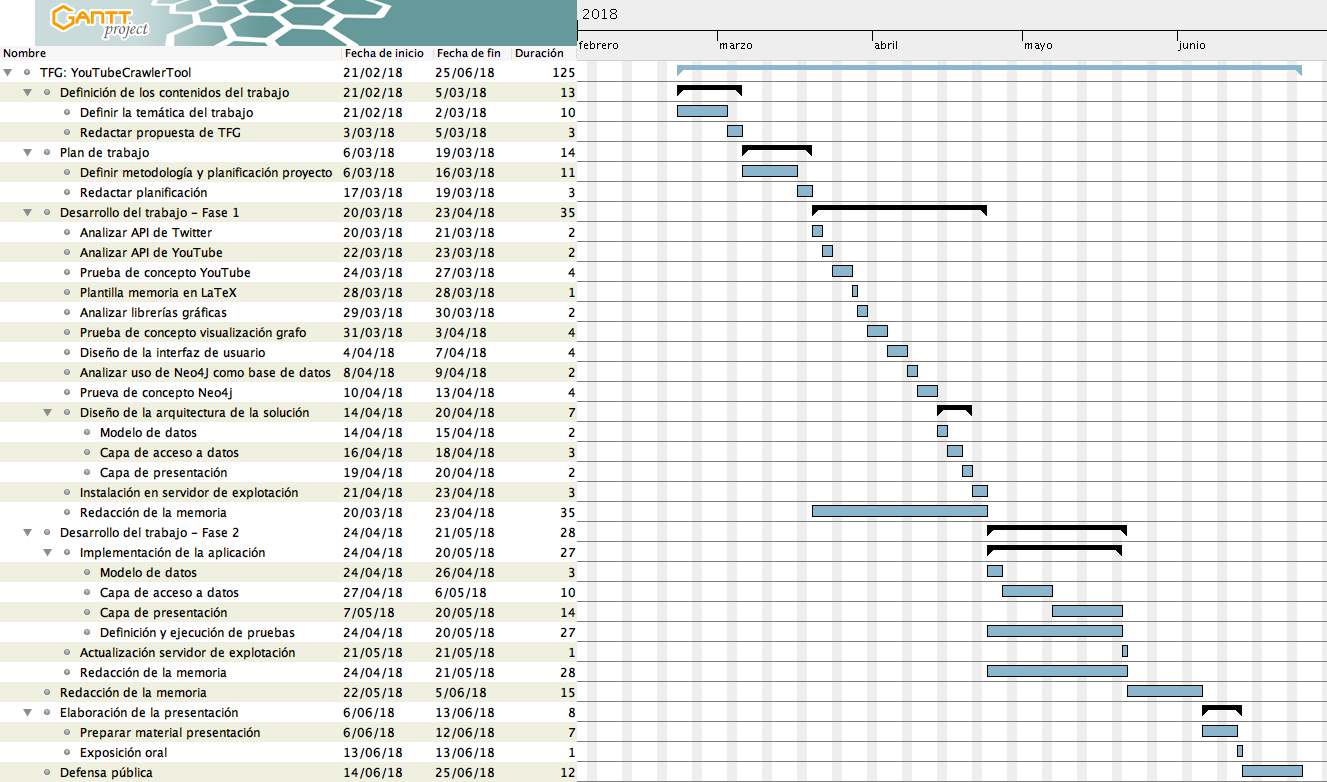
\includegraphics[scale=0.20]{planificacion/planificacion2.png}
\caption{Listado final de tareas y diagrama de Gantt}
\end{figure}

\begin{figure}[H]
\centering
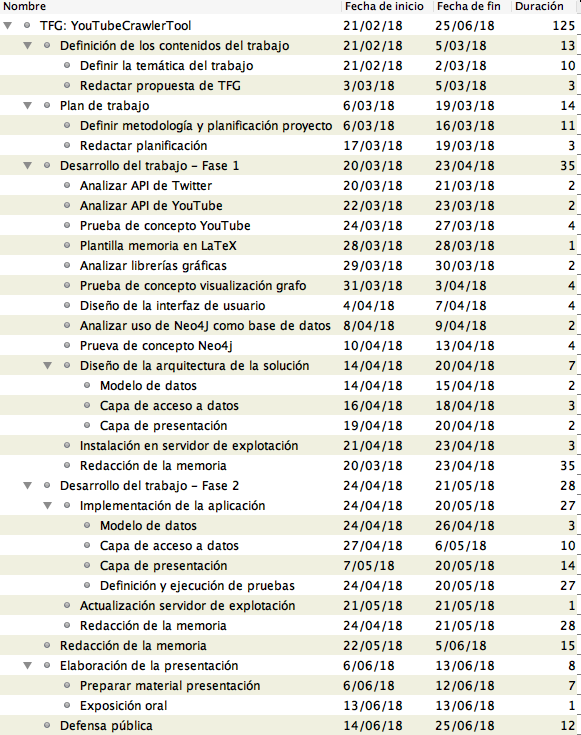
\includegraphics[scale=0.35]{planificacion/listado-tareas2.png}
\caption{Listado final de tareas}
\end{figure}

\end{itemize}


\medskip 

\subsection{Propuesta de mejoras}
Como en toda aplicación, siempre existen propuestas que pueden mejorar la calidad y la satisfacción de los usuarios sobre el producto desarrollado, las cuales pueden ser funcionales o no funcionales. Las razones por las que estas propuestas no han sido incorporadas en el producto final entregado pueden ser varias, ya sea por ejemplo por falta de tiempo asignado para su desarrollo o por quedar fuera del alcance real del proyecto.
\\

A continuación se facilita un listado de propuestas de mejora de la aplicación que fueron detectadas durante el desarrollo de la misma:
\\

\noindent\textbf{Propuestas funcionales:}
\begin{itemize}
\item \textbf{Accesibilidad y usabilidad}: El propósito principal de la capa cliente desarrollada fue la de habilitar las funcionalidades desarrolladas a la clienta de la aplicación, por lo que la interfaz de usuario diseñada y implementada se centra en este objetivo. Para asegurar que la aplicación puede usarse de forma usable por un publico más amplio, debería someterse a un estudio de experiencia de usuario que tomara también en consideración la accesibilidad de la aplicación.
\item \textbf{Añadir inteligencia artificial para la categorización de vídeos}: Ahora mismo, para mostrar grupos de contenidos bien diferenciados en el grafo se requiere realizar previamente un trabajo manual de categorización, el cual, dependiendo del volumen de datos sobre el que se requiera trabajar puede llegar a ser inviable. Para solucionar esta problemática se propone la adicción al proyecto de capacidades de inteligencia artificial que hagan posible la categorización automática de los contenidos recolectados. Como propuesta inicial a estudio, se podría considerar el uso de un modelo basado en reglas que, al aplicarlas sobre los metadatos de los vídeos (tales como titulo o descripción), se pudiera asignar automáticamente categorías a los vídeos.
\end{itemize}
\medskip 

\noindent\textbf{Propuestas no funcionales:}
\begin{itemize}
\item \textbf{Manejo de errores en la API REST:} Debido a que la API REST desarrollada inicialmente va a ser utilizada solo por un cliente web, esta no provee un manejo de errores adecuado delegando esta parte de la lógica en la interfaz web. Para que esta API pueda ser consumida por terceros o distintos tipos de clientes, esta debería proporcionar códigos y mensajes de error adecuados a cada situación.
\item \textbf{Paginación de resultados en la API REST:} Parecido al punto anterior, actualmente la paginación de resultados se realiza en la interfaz de usuario. La API desarrollada debería incorporar la funcionalidad necesaria para permitir la paginación de listados de resultados para minimizar las llamadas a la API y el ancho de banda utilizado por la aplicación.
\item \textbf{Mejorar los registros de la aplicación:} Aunque en la ejecución de la aplicación se genera un fichero de registro, la aplicación debería proporcionar mejor y un mayor nivel de registro por tal de facilitar su monitorización.
\item \textbf{Realizar filtros en la búsqueda de \textit{'Analysis'} por base de datos en vez de lógicamente:} En la consulta realizada a base de datos para la obtención de vídeos a ser presentados en el grafo, solo se realiza el filtrando de los campos obligatorios (por fecha), los demás filtros disponibles en esta funcionalidad (tales como por categoría o proceso de recolección) no son obligatorios y pueden venir informados o no. Por falta de tiempo en la investigación, no se encontró la forma de realizar consultas a \textit{Neo4J} con parámetros que podían venir informados o no, como solución temporal se decidió realizar el filtrado de los parámetros opcionales de forma lógica posteriormente a la realización de la consulta a la base de datos. Esta solución temporal puede conllevar problemas de rendimiento en el futuro y, aunque como se comenta a continuación no es el principal problema potencial de rendimiento en la visualización del grafo,  debería encontrarse una alternativa mejor. 
\item \textbf{Mejorar el rendimiento de la representación del grafo:} Tal y como se comenta en la página web oficial de la librería \textit{JavaScript Cytoscape.js} utilizada para la visualización del grafo, en los gráficos con una gran cantidad de nodos a representar el rendimiento de la librería empieza a degradarse  \cite{28}. En las pruebas realizadas se ha confirmado esta afirmación al, por ejemplo, tardar aproximadamente unos 34 segundos en visualizarse un grafo con mil nodos (4 segundos para obtener los vídeos a representar de la base de datos y a realizar el filtrado lógico de los mismos más 30 segundos para que la librería los visualice por pantalla). Debido al gran volumen de información con la que se puede trabajar con la aplicación, para mejorar el rendimiento en la visualización de grafos se deberían adoptar medidas correctoras (tales como disminuir la información a mostrar por cada nodo) o estudiar alternativas al uso de \textit{Cytoscape.js} como librería \textit{JavaScript} para la representación del grafo.
\end{itemize}
\newpage 


\section{Glosario} 
\begin{table}[H]
\begin{tabular}{ll}
ACID & \textit{Atomicity, Consistency, Isolation and Durability}                  \\
AJAX & \textit{Asynchronous JavaScript And XML}                  \\
API & \textit{Application Programming Interface}                  \\
CSV & \textit{Comma-Separated Values}                  \\
DAO & \textit{Data Access Object}                  \\
DB & \textit{DataBase}                  \\
DOM & \textit{Document Object Model}                  \\
HTTP & \textit{HyperText Transfer Protocol}                  \\
JPA & \textit{Java Persistence API}                  \\
JSON & \textit{JavaScript Object Notation}                  \\
MVC & \textit{Model–View–Controller}                  \\
NoSQL & \textit{Not Only SQL}                  \\
POC & \textit{Proof Of Concept}                  \\
POJO & \textit{Plain Old Java Object}                  \\
REST & \textit{REpresentational State Transfer}                  \\
RPC & \textit{Remote Procedure Call}                  \\
SGBD & \textit{Sistema Gestor de Base de Datos}                  \\
SQL & \textit{Structured Query Language}                  \\
TFG & \textit{Trabajo Final de Grado}                  \\
UML & \textit{Unified Modeling Language}                  \\
URI & \textit{Uniform Resource Identifier}                  \\
URL & \textit{Uniform Resource Locator}                  \\
WAR & \textit{Web Application Archive}                  \\
XML & \textit{eXtensible Markup Language}
\end{tabular}%
\end{table}
\newpage 


\section{Bibliografía}
\bigskip

\begin{thebibliography}{0}
  \bibitem{1} \url{https://es.wikipedia.org/wiki/Controversia_de_las_vacunas} (07/03/2018)
  \bibitem{2} \url{http://www.elmundo.es/cataluna/2015/06/27/558e5fb2e2704ea41e8b4576.html} (07/03/2018)
  \bibitem{3} \url{https://buenavibra.es/movida-sana/salud/italia-sarampion-movimientos-antivacunas} (16/03/2018)
  \bibitem{4} \url{https://es.wikipedia.org/wiki/Ciencia_de_datos} (07/03/2018)
  \bibitem{5} \url{https://es.wikipedia.org/wiki/Interfaz_de_programacion_de_aplicaciones} (07/03/2018)
  \bibitem{6} \url{https://es.wikipedia.org/wiki/NoSQL} (07/03/2018)
  \bibitem{7} \url{https://es.wikipedia.org/wiki/Macrodatos} (07/03/2018)
  \bibitem{8} \url{https://es.wikipedia.org/wiki/Scrum_(desarrollo_de_software)} (16/03/2018)
  \bibitem{9} \url{https://trello.com} (16/03/2018)
  \bibitem{10} \url{https://es.wikipedia.org/wiki/Base_de_datos_orientada_a_grafos} (23/05/2018)
  \bibitem{11} \url{http://www.oracle.com/technetwork/java/index.html} (23/05/2018)
  \bibitem{12} \url{https://spring.io/} (23/05/2018)
  \bibitem{13} \url{https://es.wikipedia.org/wiki/JavaScript} (23/05/2018)
  \bibitem{14} \url{https://jquery.com/} (23/05/2018)
  \bibitem{15} \url{https://es.wikipedia.org/wiki/Dise%C3%B1o_centrado_en_el_usuario} (24/05/2018)
  \bibitem{16} \url{https://es.wikipedia.org/wiki/Caso_de_uso} (24/05/2018) 
  \bibitem{17} \url{https://developer.twitter.com/en/docs/tweets/search/overview} (26/05/2018) 
  \bibitem{18} \url{https://developers.google.com/youtube/v3/getting-started?hl=es-419#quota} (26/05/2018) 
  \bibitem{19} \url{https://es.wikipedia.org/wiki/Modelo%E2%80%93vista%E2%80%93controlador} (29/05/2018) 
  \bibitem{20} \url{https://docs.microsoft.com/es-es/azure/architecture/best-practices/api-design} (29/05/2018) 
  \bibitem{21} \url{http://www.oracle.com/technetwork/java/javase/downloads/jdk8-downloads-2133151.html} (29/05/2018) 
  \bibitem{22} \url{https://git-scm.com/} (29/05/2018) 
  \bibitem{23} \url{https://maven.apache.org/} (29/05/2018) 
  \bibitem{24} \url{https://spring.io/tools} (29/05/2018) 
  \bibitem{25} \url{http://tomcat.apache.org/} (29/05/2018) 
  \bibitem{26} \url{https://projects.spring.io/spring-boot/} (29/05/2018) 
  \bibitem{27} \url{https://developers.google.com/youtube/v3/getting-started#before-you-start} (29/05/2018) 
  \bibitem{28} \url{http://js.cytoscape.org/#performance} (31/05/2018) 
  \bibitem{29} \url{https://developers.google.com/youtube/v3/} (02/06/2018) 
  \bibitem{30} \url{https://developers.google.com/youtube/v3/docs/search/list} (02/06/2018)  
  \bibitem{31} \url{https://developers.google.com/youtube/v3/docs/videos/list} (02/06/2018)  
  \bibitem{32} \url{https://developers.google.com/youtube/v3/docs/channels/list} (02/06/2018)
  \bibitem{33} \url{https://es.wikipedia.org/wiki/ACID} (02/06/2018)  
  \bibitem{34} \url{http://cassandra.apache.org/} (02/06/2018)
  \bibitem{35} \url{https://www.mongodb.com/} (02/06/2018)
  \bibitem{36} \url{http://couchdb.apache.org/} (02/06/2018)
  \bibitem{37} \url{https://neo4j.com/} (02/06/2018)
  \bibitem{38} \url{https://es.wikipedia.org/wiki/Base_de_datos_orientada_a_grafos} (02/06/2018)
  \bibitem{39} \url{https://projects.spring.io/spring-data-neo4j/} (02/06/2018) 
  \bibitem{40} \url{https://es.wikipedia.org/wiki/Java_Persistence_API} (02/06/2018) 
  \bibitem{41} \url{https://es.wikipedia.org/wiki/Objeto_de_acceso_a_datos} (02/06/2018) 
  \bibitem{42} \url{https://es.wikipedia.org/wiki/CRUD} (02/06/2018)
  \bibitem{43} \url{https://es.wikipedia.org/wiki/Plain_Old_Java_Object} (02/06/2018) 
  \bibitem{44} \url{https://es.wikipedia.org/wiki/SOLID} (02/06/2018) 
  \bibitem{45} \url{https://developers.google.com/api-client-library/java/apis/youtube/v3} (03/06/2018)
  \bibitem{46} \url{https://docs.spring.io/spring/docs/current/spring-framework-reference/web.html#mvc} (03/06/2018)
  \bibitem{47} \url{http://api.jquery.com/jquery.ajax/} (03/06/2018)
  \bibitem{48} \url{https://www.thymeleaf.org/} (03/06/2018)
  \bibitem{49} \url{https://startbootstrap.com/template-overviews/sb-admin-2/} (03/06/2018)
  \bibitem{50} \url{https://projects.spring.io/spring-security/} (03/06/2018)
  \bibitem{51} \url{http://js.cytoscape.org/} (03/06/2018)
  \bibitem{52} \url{https://d3js.org/} (03/06/2018)
  \bibitem{53} \url{http://sigmajs.org/} (03/06/2018)
\end{thebibliography}
\newpage 


\section{Anexos}
\bigskip

\subsection{Manual de instalación y requerimientos}\label{Manual} 
\noindent\textbf{Requerimientos de \textit{hardware}:}
\begin{itemize}
\item \textbf{Sistema operativo:} La aplicación puede funcionar tanto en sistemas \textit{Windows}, \textit{Linux} o \textit{Mac}, en cada caso hará falta la instalación de las distribuciones correctas según el sistema operativo escogido.
\item \textbf{Memoria RAM:} Se recomienda un mínimo de 256Mb de memoria RAM dedicados a la ejecución de la aplicación.
\item \textbf{Espacio de disco:} La aplicación en si misma tiene un peso de 30Mb en disco pero dependiendo del uso requerido de la aplicación y del volumen de información a recolectar, el espacio en disco necesario puede variar. Como dato para extrapolar, un volumen de 500 vídeos y 100 canales ocupa un espació en disco aproximado de 200Mb.
\end{itemize}

\noindent\textbf{Requerimientos de \textit{software}:}
\begin{itemize}
\item \textbf{\textit{Java JDK}:} Versión 8 o superior.
\item \textbf{\textit{Neo4J Server}:} Versión 3.3.5 o superior.
\item \textbf{Contenedor de \textit{servlets}}: Puede utilizarse cualquier distribución compatible con Java 8, por ejemplo \textit{Tomcat 8}.
\end{itemize}
\bigskip 

Los pasos para realizar la instalación de la aplicación son los siguientes:
\\

\noindent\textbf{1- Instalación de Java JDK}: Las instrucciones para la instalación de la misma pueden encontrarse detallas en la pagina web oficial: \url{https://docs.oracle.com/javase/8/docs/technotes/guides/install/install_overview.html}.
\\

\noindent\textbf{2- Instalación de \textit{Neo4J Server}}: La instalación consiste simplemente en obtener la distribución deseada y descomprimirla. Se puede arrancar como servicio ejecutando el comando: \textit{bin/neo4j start}. Una vez el servicio esta arrancado, se puede visitar su consola de administración en cualquier explorador web mediante la url  \textit{http://localhost:7474} en donde al acceder por primera vez se preguntara para crear un nuevo password para el usuario administrador \textit{"neo4j"}. Mas detalles sobre su instalación se pueden encontrar en la web oficial: \url{https://neo4j.com/docs/operations-manual/current/installation/}.
\\

\noindent\textbf{3- Instalación contenedor de \textit{servlets}}: La instalación dependerá del sistema operativo y del contenedor escogido. En el caso de \textit{Tomcat 8}: \url{https://tomcat.apache.org/tomcat-8.0-doc/setup.html}.\\

\noindent\textbf{4- Configurar conexión base de datos}: La conexión de la aplicación con la base de datos Neo4J esta configurada mediante el archivo de propiedades 'application.properties', en donde los valores por defecto son:
\begin{lstlisting}[style=C]
#Neo4j connection
spring.data.neo4j.uri=bolt://localhost
spring.data.neo4j.username=neo4j
spring.data.neo4j.password=youtubecrawlertool
\end{lstlisting}
Los valores de esta configuración se pueden sobrescribir mediante un nuevo archivo de propiedades que debe de ser indicado como opciones de Java en el inició de contenedor de \textit{servlets}:\\
\textit{JAVA\_OPTS="\--Dspring.config.location=\$location\_to\_the\_overriden\_properties"}
\\

\noindent\textbf{5- Instalar fichero WAR en el contenedor de \textit{servlets}}: El ejecutable de la aplicación Web en formato de fichero WAR se entrega junto con esta memoria. Para hacer funcionar la aplicación esta debe ser instalada en un contenedor de \textit{servlets}. Seguir las instrucciones indicadas según el contenedor escogido para realizar su instalación. En el caso de \textit{Tomcat 8}: \url{https://tomcat.apache.org/tomcat-8.0-doc/deployer-howto.html}.
\\

\noindent\textbf{6- Abrir un explorador WEB}: Y acceder a la aplicación recientemente instalada. Por defecto en \textit{Tomcat 8} si se instala la aplicación en la raíz esta esta disponible en \url{http://localhost:8080/}.

\newpage 

\subsection{Ilustraciones de la aplicación}\label{IlustracionApp} 
A continuación se incluyen imágenes ilustrativas de cada una de las vistas de la aplicación en funcionamiento:

\begin{figure}[H]
\centering
\subfigure[Login.html]{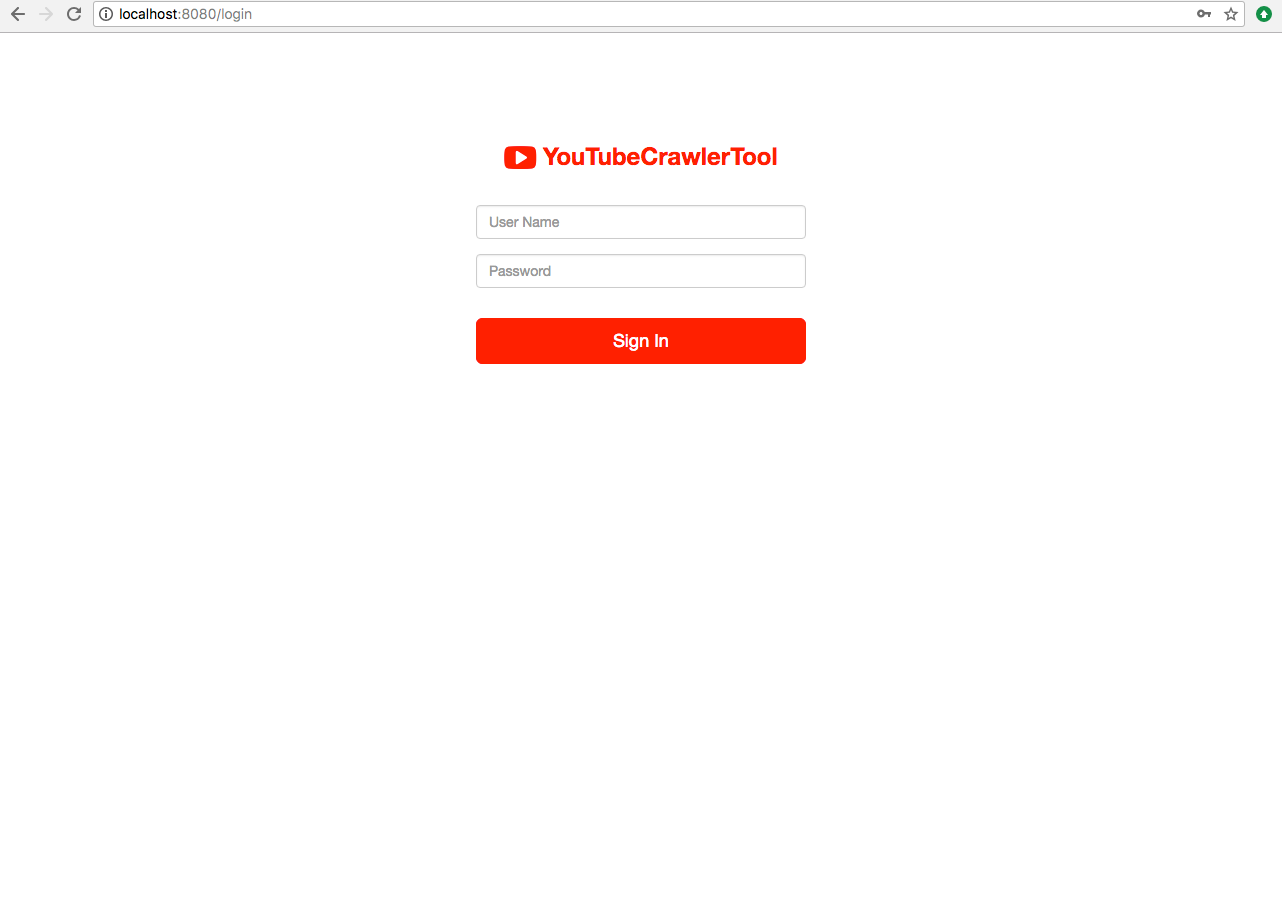
\includegraphics[width=60mm]{funcionamiento/login.png}}
\subfigure[Analysis.html]{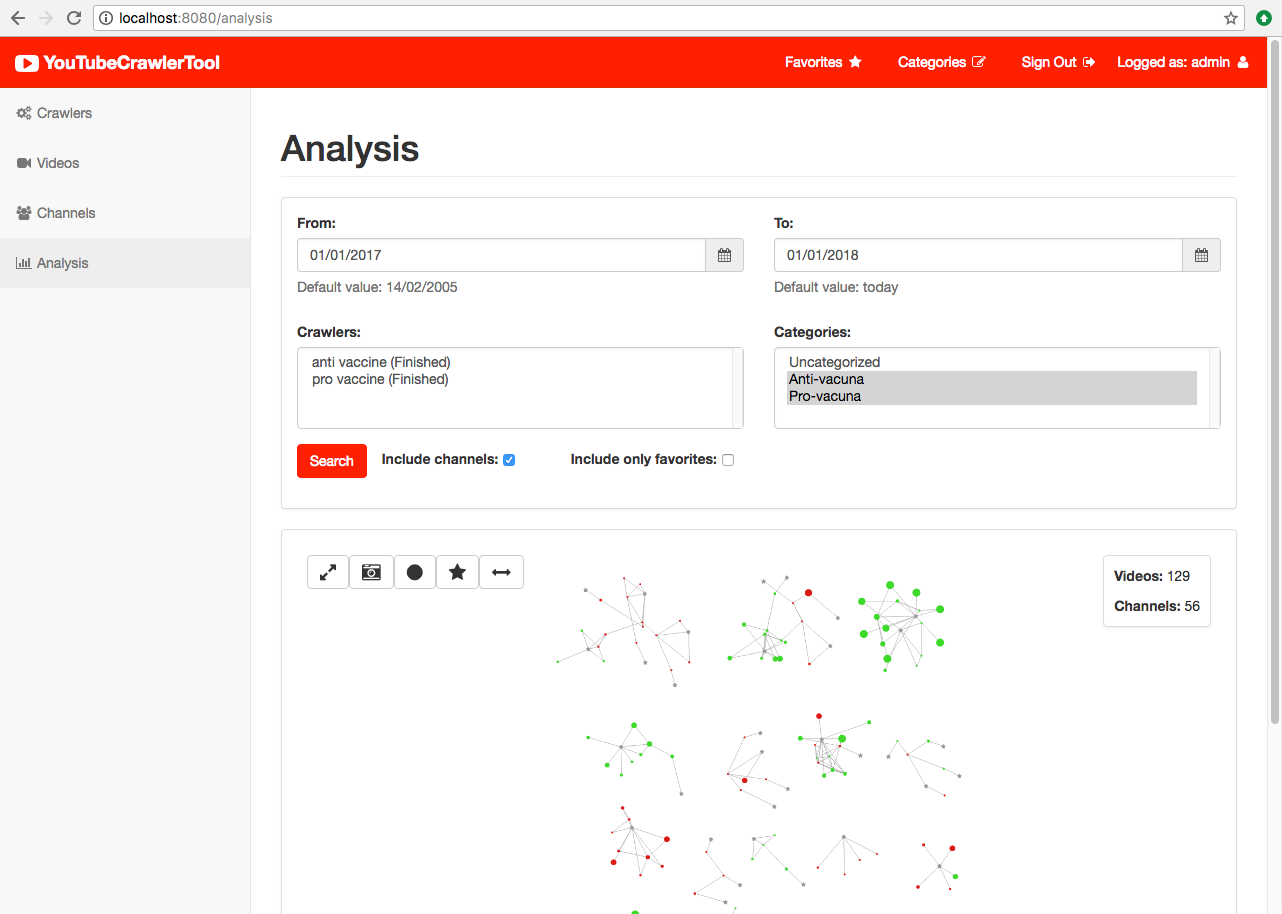
\includegraphics[width=60mm]{funcionamiento/anaysis.png}}
\end{figure}
\begin{figure}[H]
\centering
\subfigure[Crawlers.html]{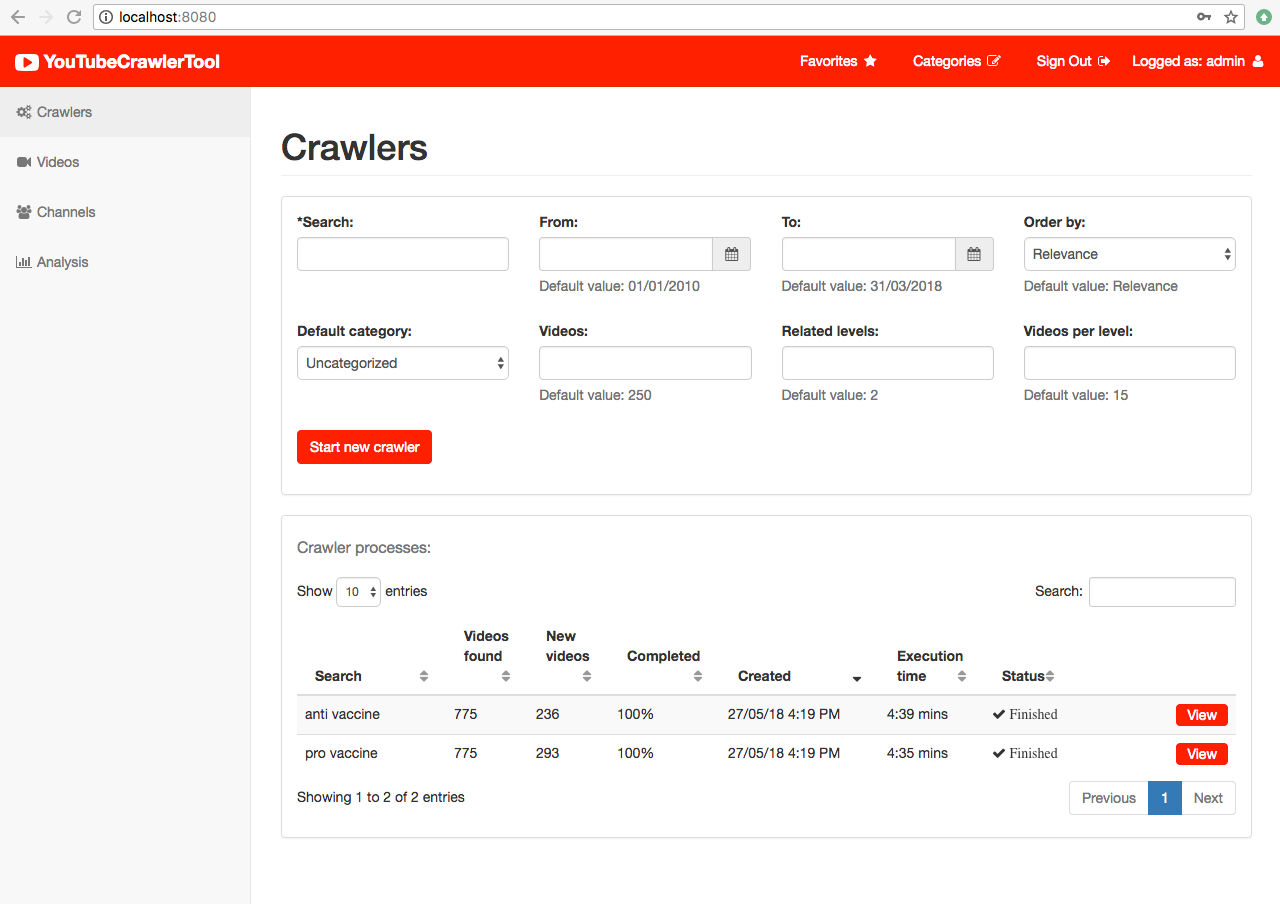
\includegraphics[width=60mm]{funcionamiento/crawlers.png}}
\subfigure[Crawler.html]{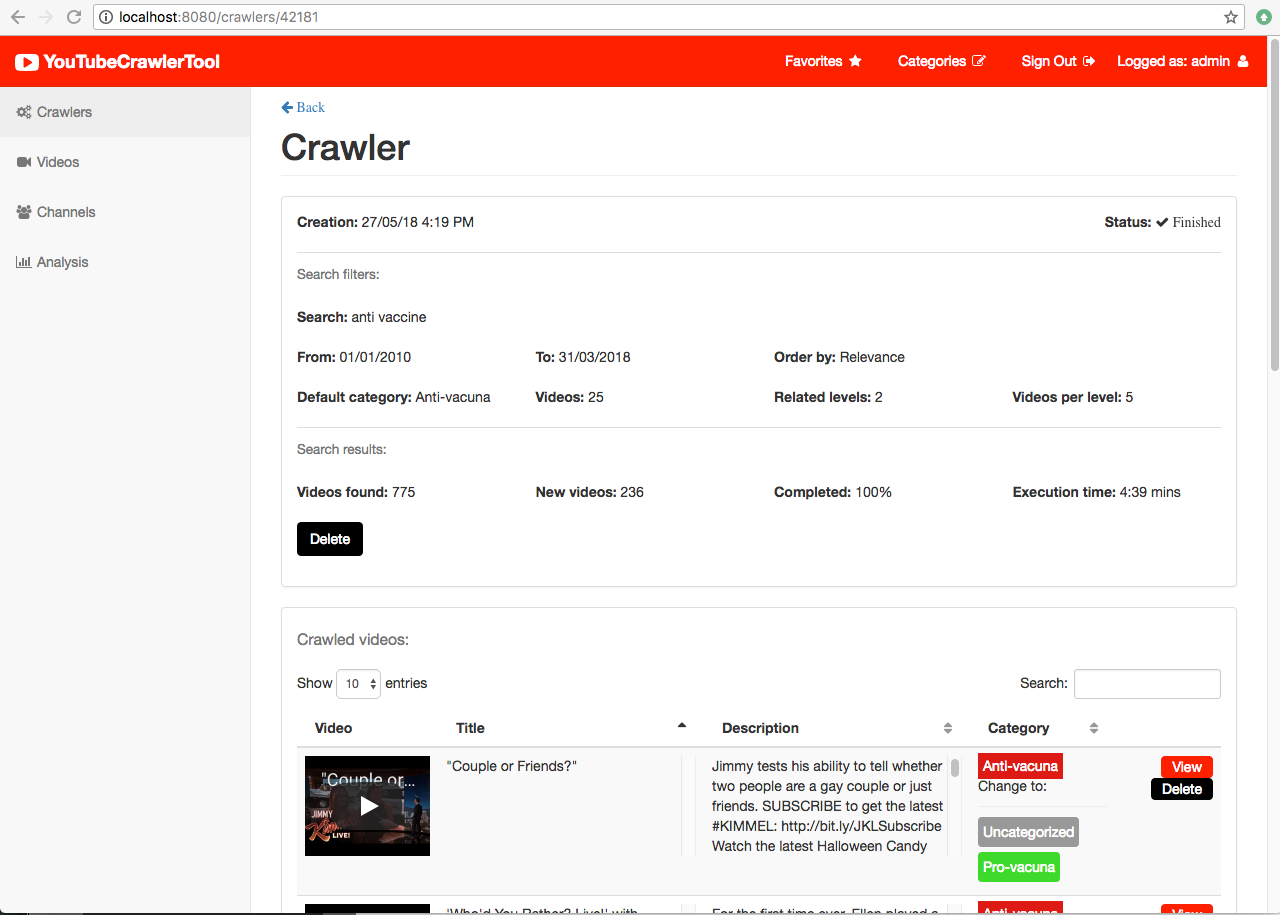
\includegraphics[width=60mm]{funcionamiento/crawler.png}}
\end{figure}
\begin{figure}[H]
\centering
\subfigure[Videos.html]{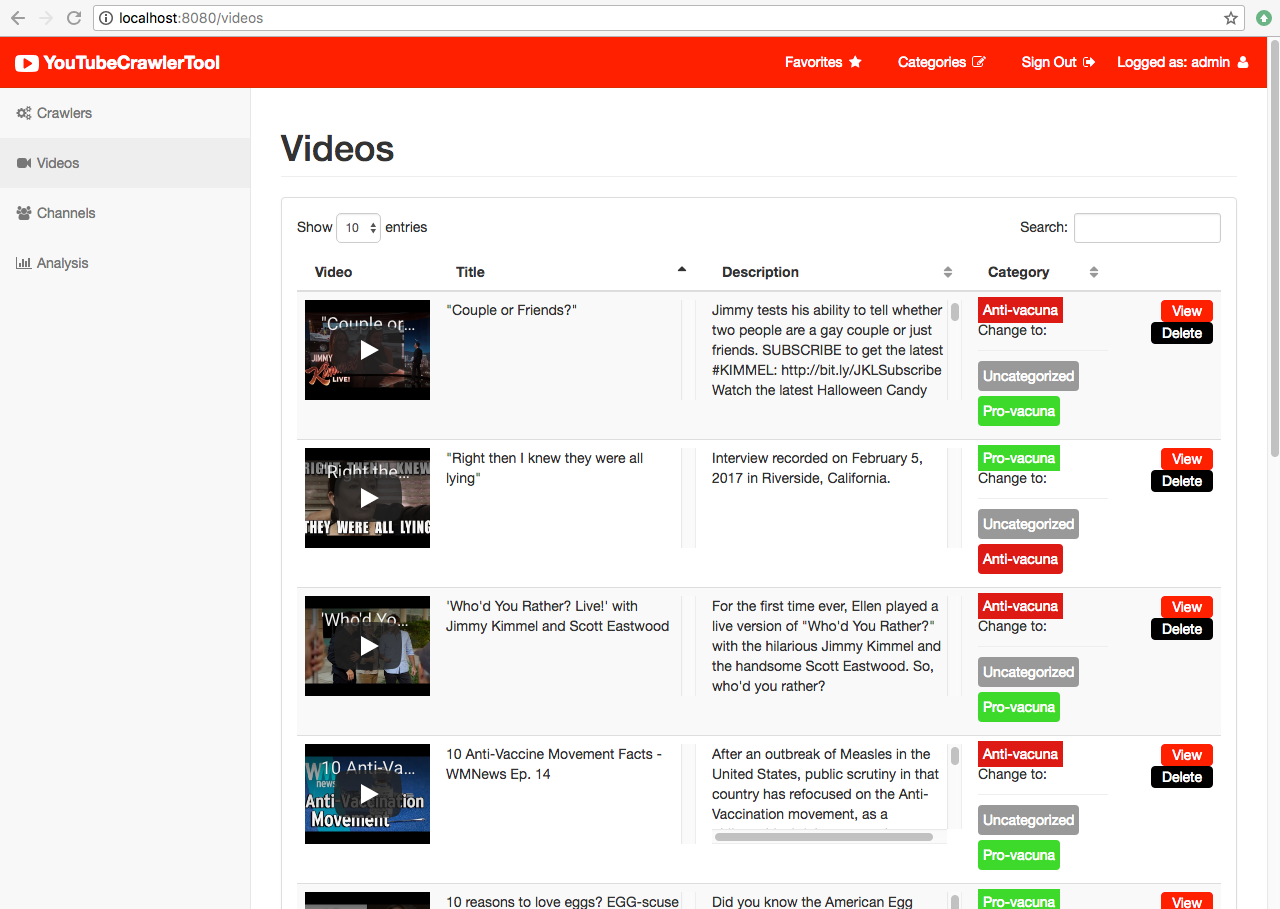
\includegraphics[width=60mm]{funcionamiento/videos.png}}
\subfigure[Video.html]{\includegraphics[width=60mm]{funcionamiento/video.png}}
\end{figure}
\begin{figure}[H]
\centering
\subfigure[Channels.html]{\includegraphics[width=60mm]{funcionamiento/channels.png}}
\subfigure[Channel.html]{\includegraphics[width=60mm]{funcionamiento/channel.png}}
\end{figure}
\begin{figure}[H]
\centering
\subfigure[Favorites.html]{\includegraphics[width=60mm]{funcionamiento/favorites.png}}
\subfigure[Categories.html]{\includegraphics[width=60mm]{funcionamiento/categories.png}}
\end{figure}
\begin{figure}[H]
\centering
\subfigure[NewCategory.html]{\includegraphics[width=60mm]{funcionamiento/newCategory.png}}
\subfigure[EditCategory.html]{\includegraphics[width=60mm]{funcionamiento/editCategory.png}}
\caption{Puesta en funcionamiento}
\end{figure}
\pagebreak 

\subsection{Pruebas de integración}\label{pruevasIntegracion} 
\begin{large}
\noindent\textbf{Resultados globales}
\end{large}

\begin{table}[H]
\centering
%\resizebox{\textwidth}{!}{%
\begin{tabular}{|c|c|c|}
\hline
\rowcolor[HTML]{C0C0C0} 
\textbf{YouTubeCrawlerTool}                                                  & \multicolumn{2}{c|}{\cellcolor[HTML]{C0C0C0}\textbf{Resultado}} \\ \hline
                                                                             & V                              & 72                             \\ \cline{2-3} 
\multirow{-2}{*}{\begin{tabular}[c]{@{}c@{}}EVALUACIÓN\\ 100\%\end{tabular}} & X                              & 0                              \\ \hline
\end{tabular}%
%}
\end{table}


\begin{large}
\noindent\textbf{Componente \textit{User session}}
\end{large}

\begin{table}[H]
\centering
\begin{tabular}{|c|c|c|}
\hline
\rowcolor[HTML]{C0C0C0} 
\textbf{User session}                                                        & \multicolumn{2}{c|}{\cellcolor[HTML]{C0C0C0}\textbf{Resultado}} \\ \hline
                                                                             & V                              & 5                              \\ \cline{2-3} 
\multirow{-2}{*}{\begin{tabular}[c]{@{}c@{}}EVALUACIÓN\\ 100\%\end{tabular}} & X                              & 0                              \\ \hline
\end{tabular}
\end{table}

\begin{table}[H]
\centering
\resizebox{\textwidth}{!}{%
\begin{tabular}{|l|l|l|c|}
\hline
\rowcolor[HTML]{FFFFFF} 
\cellcolor[HTML]{C0C0C0}\textbf{Responsable} & \multicolumn{3}{l|}{\cellcolor[HTML]{FFFFFF}Javier Sánchez Mendoza}                                                                                                                                                                                                          \\ \hline
\cellcolor[HTML]{C0C0C0}\textbf{Componente}  & \multicolumn{3}{l|}{User session}                                                                                                                                                                                                                                            \\ \hline
\cellcolor[HTML]{C0C0C0}\textbf{Caso de uso} & \multicolumn{3}{l|}{UC\_1: Login}                                                                                                                                                                                                                                            \\ \hline
\rowcolor[HTML]{C0C0C0} 
\textbf{Código}                              & {\color[HTML]{333333} \textbf{Acciones a verificar}}                                        & {\color[HTML]{333333} \textbf{Resultado esperado}}                                 & \multicolumn{1}{l|}{\cellcolor[HTML]{C0C0C0}{\color[HTML]{333333} \textbf{Verificación}}} \\ \hline
1                                            & \begin{tabular}[c]{@{}l@{}}Identificarse al sistema como\\ usuario valido.\end{tabular}     & Usuario identificado.                                                              & V                                                                                         \\ \hline
2                                            & \begin{tabular}[c]{@{}l@{}}Identificarse al sistema ya\\ estando identificado.\end{tabular} & \begin{tabular}[c]{@{}l@{}}Acción no permitida por la\\ aplicación.\end{tabular} & V                                                                                         \\ \hline
3                                            & \begin{tabular}[c]{@{}l@{}}Introducir datos nuevos o\\ incorrectos.\end{tabular}            & Usuario no identificado.                                                           & V                                                                                         \\ \hline
\multicolumn{2}{|c|}{}                                                                                                                     & \multicolumn{1}{c|}{V}                                                             & 3                                                                                         \\ \cline{3-4} 
\multicolumn{2}{|c|}{\multirow{-2}{*}{\begin{tabular}[c]{@{}c@{}}EVALUACIÓN\\ 100\%\end{tabular}}}                                         & \multicolumn{1}{c|}{X}                                                             & 0                                                                                         \\ \hline
\end{tabular}
}
\end{table}

\begin{table}[H]
\centering
\resizebox{\textwidth}{!}{%
\begin{tabular}{|l|l|l|c|}
\hline
\rowcolor[HTML]{FFFFFF} 
\cellcolor[HTML]{C0C0C0}\textbf{Responsable} & \multicolumn{3}{l|}{\cellcolor[HTML]{FFFFFF}Javier Sánchez Mendoza}                                                                                                                                                                                                          \\ \hline
\cellcolor[HTML]{C0C0C0}\textbf{Componente}  & \multicolumn{3}{l|}{User session}                                                                                                                                                                                                                                            \\ \hline
\cellcolor[HTML]{C0C0C0}\textbf{Caso de uso} & \multicolumn{3}{l|}{UC\_1-1: Logout}                                                                                                                                                                                                                                            \\ \hline
\rowcolor[HTML]{C0C0C0} 
\textbf{Código}                              & {\color[HTML]{333333} \textbf{Acciones a verificar}}                                        & {\color[HTML]{333333} \textbf{Resultado esperado}}                                 & \multicolumn{1}{l|}{\cellcolor[HTML]{C0C0C0}{\color[HTML]{333333} \textbf{Verificación}}} \\ \hline
1                                            & \begin{tabular}[c]{@{}l@{}}Cerrar sesión de un usuario\\ identificado.\end{tabular}     & \begin{tabular}[c]{@{}l@{}}El usuario actual ya no esta\\identificado en el sistema.\end{tabular} & V                                                                                         \\ \hline
2                                            & \begin{tabular}[c]{@{}l@{}}Cerrar sesión de un usuario\\ no identificado.\end{tabular} & \begin{tabular}[c]{@{}l@{}}Acción no permitida por la\\ aplicación.\end{tabular} & V                                                                                         \\ \hline
\multicolumn{2}{|c|}{}                                                                                                                     & \multicolumn{1}{c|}{V}                                                             & 2                                                                                         \\ \cline{3-4} 
\multicolumn{2}{|c|}{\multirow{-2}{*}{\begin{tabular}[c]{@{}c@{}}EVALUACIÓN\\ 100\%\end{tabular}}}                                         & \multicolumn{1}{c|}{X}                                                             & 0                                                                                         \\ \hline
\end{tabular}
}
\end{table}


\begin{large}
\noindent\textbf{Componente \textit{Crawler}}
\end{large}

\begin{table}[H]
\centering
\begin{tabular}{|c|c|c|}
\hline
\rowcolor[HTML]{C0C0C0} 
\textbf{Crawler}                                                        & \multicolumn{2}{c|}{\cellcolor[HTML]{C0C0C0}\textbf{Resultado}} \\ \hline
                                                                             & V                              & 18                              \\ \cline{2-3} 
\multirow{-2}{*}{\begin{tabular}[c]{@{}c@{}}EVALUACIÓN\\ 100\%\end{tabular}} & X                              & 0                              \\ \hline
\end{tabular}
\end{table}

\begin{table}[H]
\centering
\resizebox{\textwidth}{!}{%
\begin{tabular}{|l|l|l|l|}
\hline
\rowcolor[HTML]{FFFFFF} 
\cellcolor[HTML]{C0C0C0}\textbf{Responsable} & \multicolumn{3}{l|}{\cellcolor[HTML]{FFFFFF}Javier Sánchez Mendoza}                                                                                      \\ \hline
\cellcolor[HTML]{C0C0C0}\textbf{Componente}  & \multicolumn{3}{l|}{Crawler}                                                                                                                             \\ \hline
\cellcolor[HTML]{C0C0C0}\textbf{Caso de uso} & \multicolumn{3}{l|}{UC\_2: View all crawlers statistics}                                                                                                  \\ \hline
\rowcolor[HTML]{C0C0C0} 
\textbf{Código}                              & {\color[HTML]{333333} \textbf{Acciones a verificar}} & {\color[HTML]{333333} \textbf{Resultado esperado}} & {\color[HTML]{333333} \textbf{Verificación}} \\ \hline
\multicolumn{4}{|c|}{NO IMPLEMENTADO}                                                                                                                                                                   \\ \hline
\end{tabular}
}
\end{table}

\begin{table}[H]
\centering
\resizebox{\textwidth}{!}{%
\begin{tabular}{|l|l|l|c|}
\hline
\rowcolor[HTML]{FFFFFF} 
\cellcolor[HTML]{C0C0C0}\textbf{Responsable} & \multicolumn{3}{l|}{\cellcolor[HTML]{FFFFFF}Javier Sánchez Mendoza}                                                                                                                                                                                                                                                                                                  \\ \hline
\cellcolor[HTML]{C0C0C0}\textbf{Componente}  & \multicolumn{3}{l|}{Crawler}                                                                                                                                                                                                                                                                                                                                         \\ \hline
\cellcolor[HTML]{C0C0C0}\textbf{Caso de uso} & \multicolumn{3}{l|}{UC\_3: List all crawlers}                                                                                                                                                                                                                                                                                                                        \\ \hline
\rowcolor[HTML]{C0C0C0} 
\textbf{Código}                              & {\color[HTML]{333333} \textbf{Acciones a verificar}}                                                                                & {\color[HTML]{333333} \textbf{Resultado esperado}}                                                                                 & \multicolumn{1}{l|}{\cellcolor[HTML]{C0C0C0}{\color[HTML]{333333} \textbf{Verificación}}} \\ \hline
1                                            & \begin{tabular}[c]{@{}l@{}}Como usuario acceder al listado\\ de crawlers cuando aun no\\ existe ninguno en el sistema.\end{tabular} & \begin{tabular}[c]{@{}l@{}}No se debe mostrar ningún\\ resultado.\end{tabular}                                                    & V                                                                                         \\ \hline
2                                            & \begin{tabular}[c]{@{}l@{}}Como usuario acceder al listado\\ de crawlers cuando existen\\ algunos en el sistema.\end{tabular}       & \begin{tabular}[c]{@{}l@{}}Se debe mostrar el estado\\ actualizado de todos los crawlers\\ que existan en el sistema.\end{tabular} & V                                                                                         \\ \hline
\multicolumn{2}{|c|}{}                                                                                                                                                             & \multicolumn{1}{c|}{V}                                                                                                             & 2                                                                                         \\ \cline{3-4} 
\multicolumn{2}{|c|}{\multirow{-2}{*}{\begin{tabular}[c]{@{}c@{}}EVALUACIÓN\\ 100\%\end{tabular}}}                                                                                 & \multicolumn{1}{c|}{X}                                                                                                             & 0                                                                                         \\ \hline
\end{tabular}%
}
\end{table}

\begin{table}[H]
\centering
\resizebox{\textwidth}{!}{%
\begin{tabular}{|l|l|l|c|}
\hline
\rowcolor[HTML]{FFFFFF} 
\cellcolor[HTML]{C0C0C0}\textbf{Responsable} & \multicolumn{3}{l|}{\cellcolor[HTML]{FFFFFF}Javier Sánchez Mendoza}                                                                                                                                                                                                                                                                                                                                                                                                                         \\ \hline
\cellcolor[HTML]{C0C0C0}\textbf{Componente}  & \multicolumn{3}{l|}{Crawler}                                                                                                                                                                                                                                                                                                                                                                                                                                                                \\ \hline
\cellcolor[HTML]{C0C0C0}\textbf{Caso de uso} & \multicolumn{3}{l|}{UC\_4: Start new crawler process}                                                                                                                                                                                                                                                                                                                                                                                                                                       \\ \hline
\rowcolor[HTML]{C0C0C0} 
\textbf{Código}                              & {\color[HTML]{333333} \textbf{Acciones a verificar}}                                                                                                                                                   & {\color[HTML]{333333} \textbf{Resultado esperado}}                                                                                                                                     & \multicolumn{1}{l|}{\cellcolor[HTML]{C0C0C0}{\color[HTML]{333333} \textbf{Verificación}}} \\ \hline
1                                            & \begin{tabular}[c]{@{}l@{}}Como usuario no identificado\\ iniciar un proceso de crawler.\end{tabular}                                                                                                  & \begin{tabular}[c]{@{}l@{}}Acción no permitida por la\\ aplicación.\end{tabular}                                                                                                      & V                                                                                         \\ \hline
2                                            & \begin{tabular}[c]{@{}l@{}}Como usuario identificado\\ iniciar un nuevo proceso de\\ crawler sin indicar el termino a\\ buscar.\end{tabular}                                                           & \begin{tabular}[c]{@{}l@{}}Acción no permitida por la\\ aplicación.\end{tabular}                                                                                                      & V                                                                                         \\ \hline
3                                            & \begin{tabular}[c]{@{}l@{}}Como usuario identificado\\ iniciar un nuevo proceso de\\ crawler indicando una fecha\\ mayor en el campo “from” que\\ el que hay informado en el\\ campo “to”\end{tabular} & \begin{tabular}[c]{@{}l@{}}Acción no permitida por la\\ aplicación.\end{tabular}                                                                                                      & V                                                                                         \\ \hline
4                                            & \begin{tabular}[c]{@{}l@{}}Como usuario identificado\\ iniciar un nuevo proceso de\\ crawler indicando el termino de\\ búsqueda.\end{tabular}                                                         & \begin{tabular}[c]{@{}l@{}}Nuevo proceso de crawler\\ inicializado y almacenado con las\\ opciones introducidas o con las\\ de por defecto en los campos no\\ requeridos.\end{tabular} & V                                                                                         \\ \hline
\multicolumn{2}{|c|}{}                                                                                                                                                                                                                                & \multicolumn{1}{c|}{V}                                                                                                                                                                 & 4                                                                                         \\ \cline{3-4} 
\multicolumn{2}{|c|}{\multirow{-2}{*}{\begin{tabular}[c]{@{}c@{}}EVALUACIÓN\\ 100\%\end{tabular}}}                                                                                                                                                    & \multicolumn{1}{c|}{X}                                                                                                                                                                 & 0                                                                                         \\ \hline
\end{tabular}%
}
\end{table}

\begin{table}[H]
\centering
\resizebox{\textwidth}{!}{%
\begin{tabular}{|l|l|l|c|}
\hline
\rowcolor[HTML]{FFFFFF} 
\cellcolor[HTML]{C0C0C0}\textbf{Responsable} & \multicolumn{3}{l|}{\cellcolor[HTML]{FFFFFF}Javier Sánchez Mendoza}                                                                                                                                                                                                                                                                                                                                                                                                                                                                        \\ \hline
\cellcolor[HTML]{C0C0C0}\textbf{Componente}  & \multicolumn{3}{l|}{Crawler}                                                                                                                                                                                                                                                                                                                                                                                                                                                                                                               \\ \hline
\cellcolor[HTML]{C0C0C0}\textbf{Caso de uso} & \multicolumn{3}{l|}{UC\_5: Stop crawler process}                                                                                                                                                                                                                                                                                                                                                                                                                                                                                           \\ \hline
\rowcolor[HTML]{C0C0C0} 
\textbf{Código}                              & {\color[HTML]{333333} \textbf{Acciones a verificar}}                                                                                            & {\color[HTML]{333333} \textbf{Resultado esperado}}                                                                                                                                                                                                                                           & \multicolumn{1}{l|}{\cellcolor[HTML]{C0C0C0}{\color[HTML]{333333} \textbf{Verificación}}} \\ \hline
1                                            & \begin{tabular}[c]{@{}l@{}}Como usuario no identificado\\ parar un proceso de crawler.\end{tabular}                                             & \begin{tabular}[c]{@{}l@{}}Acción no permitida por la\\ aplicación.\end{tabular}                                                                                                                                                                                                             & V                                                                                         \\ \hline
2                                            & \begin{tabular}[c]{@{}l@{}}Como usuario identificado\\ parar un proceso de crawler\\ que este en un estado distinto\\ a “Running”.\end{tabular} & \begin{tabular}[c]{@{}l@{}}Acción no permitida por la\\ aplicación.\end{tabular}                                                                                                                                                                                                             & V                                                                                         \\ \hline
3                                            & \begin{tabular}[c]{@{}l@{}}Como usuario identificado\\ parar un proceso de crawler\\ que este en estado “Running”.\end{tabular}                 & \begin{tabular}[c]{@{}l@{}}El proceso pasa al estado\\ “Stopping” y en acabar la\\ extracción de videos de la pagina\\ actual del crawler el proceso pasa\\ al estado “Stopped” si hay mas\\ paginas para extraer, en caso\\ contrario el crawler pasa al\\ estado “Finished”.\end{tabular} & V                                                                                         \\ \hline
\multicolumn{2}{|c|}{}                                                                                                                                                                         & \multicolumn{1}{c|}{V}                                                                                                                                                                                                                                                                       & 3                                                                                         \\ \cline{3-4} 
\multicolumn{2}{|c|}{\multirow{-2}{*}{\begin{tabular}[c]{@{}c@{}}EVALUACIÓN\\ 100\%\end{tabular}}}                                                                                             & \multicolumn{1}{c|}{X}                                                                                                                                                                                                                                                                       & 0                                                                                         \\ \hline
\end{tabular}%
}
\end{table}

\begin{table}[H]
\centering
\resizebox{\textwidth}{!}{%
\begin{tabular}{|l|l|l|c|}
\hline
\rowcolor[HTML]{FFFFFF} 
\cellcolor[HTML]{C0C0C0}\textbf{Responsable} & \multicolumn{3}{l|}{\cellcolor[HTML]{FFFFFF}Javier Sánchez Mendoza}                                                                                                                                                                                                                                                                                                  \\ \hline
\cellcolor[HTML]{C0C0C0}\textbf{Componente}  & \multicolumn{3}{l|}{Crawler}                                                                                                                                                                                                                                                                                                                                         \\ \hline
\cellcolor[HTML]{C0C0C0}\textbf{Caso de uso} & \multicolumn{3}{l|}{UC\_6: Play crawler process}                                                                                                                                                                                                                                                                                                                     \\ \hline
\rowcolor[HTML]{C0C0C0} 
\textbf{Código}                              & {\color[HTML]{333333} \textbf{Acciones a verificar}}                                                                                                & {\color[HTML]{333333} \textbf{Resultado esperado}}                                                                 & \multicolumn{1}{l|}{\cellcolor[HTML]{C0C0C0}{\color[HTML]{333333} \textbf{Verificación}}} \\ \hline
1                                            & \begin{tabular}[c]{@{}l@{}}Como usuario no identificado\\ reiniciar un proceso de crawler.\end{tabular}                                             & \begin{tabular}[c]{@{}l@{}}Acción no permitida por la\\ aplicación.\end{tabular}                                   & V                                                                                         \\ \hline
2                                            & \begin{tabular}[c]{@{}l@{}}Como usuario identificado\\ reiniciar un proceso de crawler\\ que este en un estado distinto\\ a “Stopped”.\end{tabular} & \begin{tabular}[c]{@{}l@{}}Acción no permitida por la\\ aplicación.\end{tabular}                                   & V                                                                                         \\ \hline
3                                            & \begin{tabular}[c]{@{}l@{}}Como usuario identificado\\ reiniciar un proceso de crawler\\ que este en estado “Stopped”.\end{tabular}                 & \begin{tabular}[c]{@{}l@{}}El proceso pasa al estado\\ “Running” y se continua\\ recolectando videos.\end{tabular} & V                                                                                         \\ \hline
\multicolumn{2}{|c|}{}                                                                                                                                                                             & \multicolumn{1}{c|}{V}                                                                                             & 3                                                                                         \\ \cline{3-4} 
\multicolumn{2}{|c|}{\multirow{-2}{*}{\begin{tabular}[c]{@{}c@{}}EVALUACIÓN\\ 100\%\end{tabular}}}                                                                                                 & \multicolumn{1}{c|}{X}                                                                                             & 0                                                                                         \\ \hline
\end{tabular}%
}
\end{table}

\begin{table}[H]
\centering
\resizebox{\textwidth}{!}{%
\begin{tabular}{|l|l|l|c|}
\hline
\rowcolor[HTML]{FFFFFF} 
\cellcolor[HTML]{C0C0C0}\textbf{Responsable} & \multicolumn{3}{l|}{\cellcolor[HTML]{FFFFFF}Javier Sánchez Mendoza}                                                                                                                                                                                                                                                                      \\ \hline
\cellcolor[HTML]{C0C0C0}\textbf{Componente}  & \multicolumn{3}{l|}{Crawler}                                                                                                                                                                                                                                                                                                             \\ \hline
\cellcolor[HTML]{C0C0C0}\textbf{Caso de uso} & \multicolumn{3}{l|}{UC\_7: View crawler process details}                                                                                                                                                                                                                                                                                 \\ \hline
\rowcolor[HTML]{C0C0C0} 
\textbf{Código}                              & {\color[HTML]{333333} \textbf{Acciones a verificar}}                                                            & {\color[HTML]{333333} \textbf{Resultado esperado}}                                                                         & \multicolumn{1}{l|}{\cellcolor[HTML]{C0C0C0}{\color[HTML]{333333} \textbf{Verificación}}} \\ \hline
1                                            & \begin{tabular}[c]{@{}l@{}}Como usuario accedo a la vista\\ en detalle de un proceso de\\ crawler.\end{tabular} & \begin{tabular}[c]{@{}l@{}}Es posible ver la información\\ actualizada del proceso de\\ crawler seleccionado.\end{tabular} & V                                                                                         \\ \hline
\multicolumn{2}{|c|}{}                                                                                                                                         & \multicolumn{1}{c|}{V}                                                                                                     & 1                                                                                         \\ \cline{3-4} 
\multicolumn{2}{|c|}{\multirow{-2}{*}{\begin{tabular}[c]{@{}c@{}}EVALUACIÓN\\ 100\%\end{tabular}}}                                                             & \multicolumn{1}{c|}{X}                                                                                                     & 0                                                                                         \\ \hline
\end{tabular}%
}
\end{table}

\begin{table}[H]
\centering
\resizebox{\textwidth}{!}{%
\begin{tabular}{|l|l|l|l|}
\hline
\rowcolor[HTML]{FFFFFF} 
\cellcolor[HTML]{C0C0C0}\textbf{Responsable} & \multicolumn{3}{l|}{\cellcolor[HTML]{FFFFFF}Javier Sánchez Mendoza}                                                                                      \\ \hline
\cellcolor[HTML]{C0C0C0}\textbf{Componente}  & \multicolumn{3}{l|}{Crawler}                                                                                                                             \\ \hline
\cellcolor[HTML]{C0C0C0}\textbf{Caso de uso} & \multicolumn{3}{l|}{UC\_8: View crawler process statistics}                                                                                                  \\ \hline
\rowcolor[HTML]{C0C0C0} 
\textbf{Código}                              & {\color[HTML]{333333} \textbf{Acciones a verificar}} & {\color[HTML]{333333} \textbf{Resultado esperado}} & {\color[HTML]{333333} \textbf{Verificación}} \\ \hline
\multicolumn{4}{|c|}{NO IMPLEMENTADO}                                                                                                                                                                   \\ \hline
\end{tabular}
}
\end{table}

\begin{table}[H]
\centering
\resizebox{\textwidth}{!}{%
\begin{tabular}{|l|l|l|c|}
\hline
\rowcolor[HTML]{FFFFFF} 
\cellcolor[HTML]{C0C0C0}\textbf{Responsable} & \multicolumn{3}{l|}{\cellcolor[HTML]{FFFFFF}Javier Sánchez Mendoza}                                                                                                                                                                                                                                                                                                                                                                                                                     \\ \hline
\cellcolor[HTML]{C0C0C0}\textbf{Componente}  & \multicolumn{3}{l|}{Crawler}                                                                                                                                                                                                                                                                                                                                                                                                                                                            \\ \hline
\cellcolor[HTML]{C0C0C0}\textbf{Caso de uso} & \multicolumn{3}{l|}{UC\_9: Delete crawler process}                                                                                                                                                                                                                                                                                                                                                                                                                                      \\ \hline
\rowcolor[HTML]{C0C0C0} 
\textbf{Código}                              & {\color[HTML]{333333} \textbf{Acciones a verificar}}                                                                                                         & {\color[HTML]{333333} \textbf{Resultado esperado}}                                                                                                                                                                           & \multicolumn{1}{l|}{\cellcolor[HTML]{C0C0C0}{\color[HTML]{333333} \textbf{Verificación}}} \\ \hline
1                                            & \begin{tabular}[c]{@{}l@{}}Como usuario no identificado\\ eliminar un proceso de crawler.\end{tabular}                                                       & \begin{tabular}[c]{@{}l@{}}Acción no permitida por la\\ aplicación.\end{tabular}                                                                                                                                             & V                                                                                         \\ \hline
2                                            & \begin{tabular}[c]{@{}l@{}}Como usuario identificado\\ eliminar un proceso de crawler\\ en estado “Running” o\\ “Stopping\end{tabular}                       & \begin{tabular}[c]{@{}l@{}}Acción no permitida por la\\ aplicación.\end{tabular}                                                                                                                                             & V                                                                                         \\ \hline
3                                            & \begin{tabular}[c]{@{}l@{}}Como usuario identificado\\ eliminar un proceso de crawler\\ en estado “Finished”,\\ “Stopped”, “Blocked” o “Error”.\end{tabular} & \begin{tabular}[c]{@{}l@{}}El proceso de crawler como los\\ vídeos que ha recolectado son\\ eliminados del sistema además de\\ los canales que como resultado\\ de la acción no tengan ningún\\ vídeo asociado.\end{tabular} & V                                                                                         \\ \hline
\multicolumn{2}{|c|}{}                                                                                                                                                                                      & \multicolumn{1}{c|}{V}                                                                                                                                                                                                       & 3                                                                                         \\ \cline{3-4} 
\multicolumn{2}{|c|}{\multirow{-2}{*}{\begin{tabular}[c]{@{}c@{}}EVALUACIÓN\\ 100\%\end{tabular}}}                                                                                                          & \multicolumn{1}{c|}{X}                                                                                                                                                                                                       & 0                                                                                         \\ \hline
\end{tabular}%
}
\end{table}

\begin{table}[H]
\centering
\resizebox{\textwidth}{!}{%
\begin{tabular}{|l|l|l|c|}
\hline
\rowcolor[HTML]{FFFFFF} 
\cellcolor[HTML]{C0C0C0}\textbf{Responsable} & \multicolumn{3}{l|}{\cellcolor[HTML]{FFFFFF}Javier Sánchez Mendoza}                                                                                                                                                                                                                                                                                                                               \\ \hline
\cellcolor[HTML]{C0C0C0}\textbf{Componente}  & \multicolumn{3}{l|}{Crawler}                                                                                                                                                                                                                                                                                                                                                                      \\ \hline
\cellcolor[HTML]{C0C0C0}\textbf{Caso de uso} & \multicolumn{3}{l|}{CU\_10: List all crawler process videos}                                                                                                                                                                                                                                                                                                                                      \\ \hline
\rowcolor[HTML]{C0C0C0} 
\textbf{Código}                              & {\color[HTML]{333333} \textbf{Acciones a verificar}}                                                                                                                   & {\color[HTML]{333333} \textbf{Resultado esperado}}                                                                           & \multicolumn{1}{l|}{\cellcolor[HTML]{C0C0C0}{\color[HTML]{333333} \textbf{Verificación}}} \\ \hline
1                                            & \begin{tabular}[c]{@{}l@{}}Como usuario acceder al listado\\ de videos recolectados por un\\ crawler cuando el crawler no\\ ha recolectado ningún vídeo.\end{tabular} & \begin{tabular}[c]{@{}l@{}}No se debe mostrar ningún\\ resultado.\end{tabular}                                               & V                                                                                         \\ \hline
2                                            & \begin{tabular}[c]{@{}l@{}}Como usuario acceder al listado\\ de videos recolectados por un\\ crawler cuando el crawler ha\\ recolectado algún vídeo.\end{tabular}     & \begin{tabular}[c]{@{}l@{}}Se deben mostrar todos y solo los\\ vídeos recolectados por el\\ proceso de crawler.\end{tabular} & V                                                                                         \\ \hline
\multicolumn{2}{|c|}{}                                                                                                                                                                                                & \multicolumn{1}{c|}{V}                                                                                                       & 2                                                                                         \\ \cline{3-4} 
\multicolumn{2}{|c|}{\multirow{-2}{*}{\begin{tabular}[c]{@{}c@{}}EVALUACIÓN\\ 100\%\end{tabular}}}                                                                                                                    & \multicolumn{1}{c|}{X}                                                                                                       & 0                                                                                         \\ \hline
\end{tabular}%
}
\end{table}



\begin{large}
\noindent\textbf{Componente \textit{Video}}
\end{large}

\begin{table}[H]
\centering
\begin{tabular}{|c|c|c|}
\hline
\rowcolor[HTML]{C0C0C0} 
\textbf{Video}                                                        & \multicolumn{2}{c|}{\cellcolor[HTML]{C0C0C0}\textbf{Resultado}} \\ \hline
                                                                             & V                              & 22                              \\ \cline{2-3} 
\multirow{-2}{*}{\begin{tabular}[c]{@{}c@{}}EVALUACIÓN\\ 100\%\end{tabular}} & X                              & 0                              \\ \hline
\end{tabular}
\end{table}

\begin{table}[H]
\centering
\resizebox{\textwidth}{!}{%
\begin{tabular}{|l|l|l|c|}
\hline
\rowcolor[HTML]{FFFFFF} 
\cellcolor[HTML]{C0C0C0}\textbf{Responsable} & \multicolumn{3}{l|}{\cellcolor[HTML]{FFFFFF}Javier Sánchez Mendoza}                                                                                                                                                                                                                                                                    \\ \hline
\cellcolor[HTML]{C0C0C0}\textbf{Componente}  & \multicolumn{3}{l|}{Video}                                                                                                                                                                                                                                                                                                             \\ \hline
\cellcolor[HTML]{C0C0C0}\textbf{Caso de uso} & \multicolumn{3}{l|}{CU\_11-1: List all videos}                                                                                                                                                                                                                                                                                         \\ \hline
\rowcolor[HTML]{C0C0C0} 
\textbf{Código}                              & {\color[HTML]{333333} \textbf{Acciones a verificar}}                                                                              & {\color[HTML]{333333} \textbf{Resultado esperado}}                                                     & \multicolumn{1}{l|}{\cellcolor[HTML]{C0C0C0}{\color[HTML]{333333} \textbf{Verificación}}} \\ \hline
1                                            & \begin{tabular}[c]{@{}l@{}}Como usuario acceder al listado\\ de vídeos cuando aun no existe\\ ninguno en el sistema.\end{tabular} & \begin{tabular}[c]{@{}l@{}}No se debe mostrar ningún\\ resultado.\end{tabular}                         & V                                                                                         \\ \hline
2                                            & \begin{tabular}[c]{@{}l@{}}Como usuario acceder al listado\\ de vídeos cuando existen\\ algunos en el sistema.\end{tabular}       & \begin{tabular}[c]{@{}l@{}}Se deben mostrar todos los\\ vídeos que existan en el sistema.\end{tabular} & V                                                                                         \\ \hline
\multicolumn{2}{|c|}{}                                                                                                                                                           & \multicolumn{1}{c|}{V}                                                                                 & 2                                                                                         \\ \cline{3-4} 
\multicolumn{2}{|c|}{\multirow{-2}{*}{\begin{tabular}[c]{@{}c@{}}EVALUACIÓN\\ 100\%\end{tabular}}}                                                                               & \multicolumn{1}{c|}{X}                                                                                 & 0                                                                                         \\ \hline
\end{tabular}%
}
\end{table}

\begin{table}[H]
\centering
\resizebox{\textwidth}{!}{%
\begin{tabular}{|l|l|l|c|}
\hline
\rowcolor[HTML]{FFFFFF} 
\cellcolor[HTML]{C0C0C0}\textbf{Responsable} & \multicolumn{3}{l|}{\cellcolor[HTML]{FFFFFF}Javier Sánchez Mendoza}                                                                                                                                                                                                                             \\ \hline
\cellcolor[HTML]{C0C0C0}\textbf{Componente}  & \multicolumn{3}{l|}{Video}                                                                                                                                                                                                                                                                      \\ \hline
\cellcolor[HTML]{C0C0C0}\textbf{Caso de uso} & \multicolumn{3}{l|}{CU\_11: View video detail}                                                                                                                                                                                                                                                  \\ \hline
\rowcolor[HTML]{C0C0C0} 
\textbf{Código}                              & {\color[HTML]{333333} \textbf{Acciones a verificar}}                                              & {\color[HTML]{333333} \textbf{Resultado esperado}}                                              & \multicolumn{1}{l|}{\cellcolor[HTML]{C0C0C0}{\color[HTML]{333333} \textbf{Verificación}}} \\ \hline
1                                            & \begin{tabular}[c]{@{}l@{}}Como usuario acceder a la vista\\ en detalle de un video.\end{tabular} & \begin{tabular}[c]{@{}l@{}}Es posible ver la información del\\ video seleccionado.\end{tabular} & V                                                                                         \\ \hline
\multicolumn{2}{|c|}{}                                                                                                                           & \multicolumn{1}{c|}{V}                                                                          & 1                                                                                         \\ \cline{3-4} 
\multicolumn{2}{|c|}{\multirow{-2}{*}{\begin{tabular}[c]{@{}c@{}}EVALUACIÓN\\ 100\%\end{tabular}}}                                               & \multicolumn{1}{c|}{X}                                                                          & 0                                                                                         \\ \hline
\end{tabular}%
}
\end{table}

\begin{table}[H]
\centering
\resizebox{\textwidth}{!}{%
\begin{tabular}{|l|l|l|c|}
\hline
\rowcolor[HTML]{FFFFFF} 
\cellcolor[HTML]{C0C0C0}\textbf{Responsable} & \multicolumn{3}{l|}{\cellcolor[HTML]{FFFFFF}Javier Sánchez Mendoza}                                                                                                                                                                                                                                           \\ \hline
\cellcolor[HTML]{C0C0C0}\textbf{Componente}  & \multicolumn{3}{l|}{Video}                                                                                                                                                                                                                                                                                    \\ \hline
\cellcolor[HTML]{C0C0C0}\textbf{Caso de uso} & \multicolumn{3}{l|}{CU\_12: Categorize a video}                                                                                                                                                                                                                                                               \\ \hline
\rowcolor[HTML]{C0C0C0} 
\textbf{Código}                              & {\color[HTML]{333333} \textbf{Acciones a verificar}}                                                        & {\color[HTML]{333333} \textbf{Resultado esperado}}                                                  & \multicolumn{1}{l|}{\cellcolor[HTML]{C0C0C0}{\color[HTML]{333333} \textbf{Verificación}}} \\ \hline
1                                            & \begin{tabular}[c]{@{}l@{}}Como usuario no identificado\\ cambiar la categoría de un\\ vídeo.\end{tabular} & \begin{tabular}[c]{@{}l@{}}Acción no permitida por la\\ aplicación.\end{tabular}                    & V                                                                                         \\ \hline
2                                            & \begin{tabular}[c]{@{}l@{}}Como usuario identificado\\ cambiar la categoría de un\\ vídeo.\end{tabular}    & \begin{tabular}[c]{@{}l@{}}El vídeo tiene asignada la nueva\\ categoría seleccionada.\end{tabular} & V                                                                                         \\ \hline
\multicolumn{2}{|c|}{}                                                                                                                                     & \multicolumn{1}{c|}{V}                                                                              & 2                                                                                         \\ \cline{3-4} 
\multicolumn{2}{|c|}{\multirow{-2}{*}{\begin{tabular}[c]{@{}c@{}}EVALUACIÓN\\ 100\%\end{tabular}}}                                                         & \multicolumn{1}{c|}{X}                                                                              & 0                                                                                         \\ \hline
\end{tabular}%
}
\end{table}

\begin{table}[H]
\centering
\resizebox{\textwidth}{!}{%
\begin{tabular}{|l|l|l|c|}
\hline
\rowcolor[HTML]{FFFFFF} 
\cellcolor[HTML]{C0C0C0}\textbf{Responsable}                                     & \multicolumn{3}{l|}{\cellcolor[HTML]{FFFFFF}Javier Sánchez Mendoza}                                                                                                                                                                                                                                                                                 \\ \hline
\cellcolor[HTML]{C0C0C0}\textbf{Componente}                                      & \multicolumn{3}{l|}{Video}                                                                                                                                                                                                                                                                                                                          \\ \hline
\cellcolor[HTML]{C0C0C0}\textbf{Caso de uso}                                     & \multicolumn{3}{l|}{CU\_13: Delete a video}                                                                                                                                                                                                                                                                                                         \\ \hline
\rowcolor[HTML]{C0C0C0} 
\textbf{Código}                                                                  & {\color[HTML]{333333} \textbf{Acciones a verificar}}                                                                                    & {\color[HTML]{333333} \textbf{Resultado esperado}}                                                            & \multicolumn{1}{l|}{\cellcolor[HTML]{C0C0C0}{\color[HTML]{333333} \textbf{Verificación}}} \\ \hline
1                                                                                & \begin{tabular}[c]{@{}l@{}}Como usuario no identificado\\ eliminar un vídeo.\end{tabular}                                               & \begin{tabular}[c]{@{}l@{}}Acción no permitida por la\\ aplicación.\end{tabular}                              & V                                                                                         \\ \hline
2                                                                                & \begin{tabular}[c]{@{}l@{}}Como usuario identificado\\ borrar un vídeo.\end{tabular}                                                    & \begin{tabular}[c]{@{}l@{}}Acción no permitida por la\\ aplicación.\end{tabular}                              & V                                                                                         \\ \hline
3                                                                                & \begin{tabular}[c]{@{}l@{}}Como usuario identificado\\ borrar un vídeo el cual su canal\\ solo contiene el video a borrar.\end{tabular} & \begin{tabular}[c]{@{}l@{}}El vídeo ya no esta disponible en\\ el sistema al igual que su canal.\end{tabular} & V                                                                                         \\ \hline
\multicolumn{1}{|c|}{\begin{tabular}[c]{@{}c@{}}EVALUACIÓN\\ 100\%\end{tabular}} & \multicolumn{1}{c|}{}                                                                                                                   & \multicolumn{1}{c|}{V}                                                                                        & 3                                                                                         \\ \hline
\multicolumn{1}{|c|}{}                                                           & \multicolumn{1}{c|}{}                                                                                                                   & \multicolumn{1}{c|}{X}                                                                                        & 0                                                                                         \\ \hline
\end{tabular}%
}
\end{table}

\begin{table}[H]
\centering
\resizebox{\textwidth}{!}{%
\begin{tabular}{|l|l|l|c|}
\hline
\rowcolor[HTML]{FFFFFF} 
\cellcolor[HTML]{C0C0C0}\textbf{Responsable}                                     & \multicolumn{3}{l|}{\cellcolor[HTML]{FFFFFF}Javier Sánchez Mendoza}                                                                                                                                                                                                                                                                                                                                    \\ \hline
\cellcolor[HTML]{C0C0C0}\textbf{Componente}                                      & \multicolumn{3}{l|}{Video}                                                                                                                                                                                                                                                                                                                                                                             \\ \hline
\cellcolor[HTML]{C0C0C0}\textbf{Caso de uso}                                     & \multicolumn{3}{l|}{CU\_14: List all related videos}                                                                                                                                                                                                                                                                                                                                                   \\ \hline
\rowcolor[HTML]{C0C0C0} 
\textbf{Código}                                                                  & {\color[HTML]{333333} \textbf{Acciones a verificar}}                                                                                                                 & {\color[HTML]{333333} \textbf{Resultado esperado}}                                                                                  & \multicolumn{1}{l|}{\cellcolor[HTML]{C0C0C0}{\color[HTML]{333333} \textbf{Verificación}}} \\ \hline
1                                                                                & \begin{tabular}[c]{@{}l@{}}Como usuario acceder al listado\\ de vídeos relacionados de un\\ vídeo cuando el vídeo no tiene\\ ningún vídeo relacionado.\end{tabular} & \begin{tabular}[c]{@{}l@{}}No se debe mostrar ningún\\ resultado.\end{tabular}                                                      & V                                                                                         \\ \hline
2                                                                                & \begin{tabular}[c]{@{}l@{}}Como usuario acceder al listado\\ de vídeos relacionados de un\\ vídeo cuando el vídeo si tiene\\ algún vídeo relacionado.\end{tabular}  & \begin{tabular}[c]{@{}l@{}}Se deben mostrar todos y solo los\\ vídeos a los cuales el vídeo actual\\ este relacionado.\end{tabular} & V                                                                                         \\ \hline
\multicolumn{1}{|c|}{\begin{tabular}[c]{@{}c@{}}EVALUACIÓN\\ 100\%\end{tabular}} & \multicolumn{1}{c|}{}                                                                                                                                                & \multicolumn{1}{c|}{V}                                                                                                              & 2                                                                                         \\ \hline
\multicolumn{1}{|c|}{}                                                           & \multicolumn{1}{c|}{}                                                                                                                                                & \multicolumn{1}{c|}{X}                                                                                                              & 0                                                                                         \\ \hline
\end{tabular}%
}
\end{table}

\begin{table}[H]
\centering
\resizebox{\textwidth}{!}{%
\begin{tabular}{|l|l|l|c|}
\hline
\rowcolor[HTML]{FFFFFF} 
\cellcolor[HTML]{C0C0C0}\textbf{Responsable} & \multicolumn{3}{l|}{\cellcolor[HTML]{FFFFFF}Javier Sánchez Mendoza}                                                                                                                                                                                                                                                                                                                                                                                                                                             \\ \hline
\cellcolor[HTML]{C0C0C0}\textbf{Componente}  & \multicolumn{3}{l|}{Video}                                                                                                                                                                                                                                                                                                                                                                                                                                                                                      \\ \hline
\cellcolor[HTML]{C0C0C0}\textbf{Caso de uso} & \multicolumn{3}{l|}{CU\_15: Find more related videos}                                                                                                                                                                                                                                                                                                                                                                                                                                                           \\ \hline
\rowcolor[HTML]{C0C0C0} 
\textbf{Código}                              & {\color[HTML]{333333} \textbf{Acciones a verificar}}                                                                                                                                                                    & {\color[HTML]{333333} \textbf{Resultado esperado}}                                                                                                                                        & \multicolumn{1}{l|}{\cellcolor[HTML]{C0C0C0}{\color[HTML]{333333} \textbf{Verificación}}} \\ \hline
1                                            & \begin{tabular}[c]{@{}l@{}}Como usuario no identificado\\ iniciar un nuevo proceso de\\ crawler sobre un vídeo para\\ encontrar vídeos relacionados.\end{tabular}                                                       & \begin{tabular}[c]{@{}l@{}}Acción no permitida por la\\ aplicación.\end{tabular}                                                                                                          & V                                                                                         \\ \hline
2                                            & \begin{tabular}[c]{@{}l@{}}Como usuario identificado\\ iniciar un nuevo proceso de\\ crawler indicando los\\ parámetros de búsqueda sobre\\ un vídeo en concreto para\\ encontrar sus relacionados.\end{tabular}      & \begin{tabular}[c]{@{}l@{}}Un nuevo proceso de crawler de\\ búsqueda relacionada debe\\ haberse dado de alta con la\\ información introducida y estar\\ un funcionamiento.\end{tabular} & V                                                                                         \\ \hline
3                                            & \begin{tabular}[c]{@{}l@{}}Como usuario identificado\\ iniciar un nuevo proceso de\\ crawler sin indicar ningún\\ parámetro de búsqueda sobre\\ un vídeo en concreto para\\ encontrar sus relacionados.\end{tabular} & \begin{tabular}[c]{@{}l@{}}Un nuevo proceso de crawler de\\ búsqueda relacionada debe\\ haberse dado de alta con los\\ parámetros por defecto y estar un\\ funcionamiento.\end{tabular} & V                                                                                         \\ \hline
\multicolumn{2}{|c|}{}                                                                                                                                                                                                                                                 & \multicolumn{1}{c|}{V}                                                                                                                                                                    & 3                                                                                         \\ \cline{3-4} 
\multicolumn{2}{|c|}{\multirow{-2}{*}{\begin{tabular}[c]{@{}c@{}}EVALUACIÓN\\ 100\%\end{tabular}}}                                                                                                                                                                     & \multicolumn{1}{c|}{X}                                                                                                                                                                    & 0                                                                                         \\ \hline
\end{tabular}%
}
\end{table}

\begin{table}[H]
\centering
\resizebox{\textwidth}{!}{%
\begin{tabular}{|l|l|l|c|}
\hline
\rowcolor[HTML]{FFFFFF} 
\cellcolor[HTML]{C0C0C0}\textbf{Responsable} & \multicolumn{3}{l|}{\cellcolor[HTML]{FFFFFF}Javier Sánchez Mendoza}                                                                                                                                                                                                                                                                                        \\ \hline
\cellcolor[HTML]{C0C0C0}\textbf{Componente}  & \multicolumn{3}{l|}{Video}                                                                                                                                                                                                                                                                                                                                 \\ \hline
\cellcolor[HTML]{C0C0C0}\textbf{Caso de uso} & \multicolumn{3}{l|}{CU\_15-1: Add a video as a favorite}                                                                                                                                                                                                                                                                                                   \\ \hline
\rowcolor[HTML]{C0C0C0} 
\textbf{Código}                              & {\color[HTML]{333333} \textbf{Acciones a verificar}}                                                                                              & {\color[HTML]{333333} \textbf{Resultado esperado}}                                                         & \multicolumn{1}{l|}{\cellcolor[HTML]{C0C0C0}{\color[HTML]{333333} \textbf{Verificación}}} \\ \hline
1                                            & \begin{tabular}[c]{@{}l@{}}Como usuario no identificado\\ marcar un vídeo como favorito.\end{tabular}                                             & \begin{tabular}[c]{@{}l@{}}Acción no permitida por la\\ aplicación.\end{tabular}                           & V                                                                                         \\ \hline
2                                            & \begin{tabular}[c]{@{}l@{}}Como usuario identificado\\ marcar un vídeo como favorito\\ un vídeo que ya esta marcado\\ como favorito.\end{tabular} & \begin{tabular}[c]{@{}l@{}}Acción no permitida por la\\ aplicación.\end{tabular}                           & V                                                                                         \\ \hline
3                                            & \begin{tabular}[c]{@{}l@{}}Como usuario identificado\\ marcar un vídeo como favorito.\end{tabular}                                                & \begin{tabular}[c]{@{}l@{}}El vídeo es añadido al listado de\\ vídeos favoritos del usuario.\end{tabular} & V                                                                                         \\ \hline
\multicolumn{2}{|c|}{}                                                                                                                                                                           & \multicolumn{1}{c|}{V}                                                                                     & 3                                                                                         \\ \cline{3-4} 
\multicolumn{2}{|c|}{\multirow{-2}{*}{\begin{tabular}[c]{@{}c@{}}EVALUACIÓN\\ 100\%\end{tabular}}}                                                                                               & \multicolumn{1}{c|}{X}                                                                                     & 0                                                                                         \\ \hline
\end{tabular}%
}
\end{table}

\begin{table}[H]
\centering
\resizebox{\textwidth}{!}{%
\begin{tabular}{|l|l|l|c|}
\hline
\rowcolor[HTML]{FFFFFF} 
\cellcolor[HTML]{C0C0C0}\textbf{Responsable} & \multicolumn{3}{l|}{\cellcolor[HTML]{FFFFFF}Javier Sánchez Mendoza}                                                                                                                                                                                                                                                                                           \\ \hline
\cellcolor[HTML]{C0C0C0}\textbf{Componente}  & \multicolumn{3}{l|}{Video}                                                                                                                                                                                                                                                                                                                                    \\ \hline
\cellcolor[HTML]{C0C0C0}\textbf{Caso de uso} & \multicolumn{3}{l|}{CU\_15-2: Delete a video as a favorite}                                                                                                                                                                                                                                                                                                   \\ \hline
\rowcolor[HTML]{C0C0C0} 
\textbf{Código}                              & {\color[HTML]{333333} \textbf{Acciones a verificar}}                                                                                                & {\color[HTML]{333333} \textbf{Resultado esperado}}                                                          & \multicolumn{1}{l|}{\cellcolor[HTML]{C0C0C0}{\color[HTML]{333333} \textbf{Verificación}}} \\ \hline
1                                            & \begin{tabular}[c]{@{}l@{}}Como usuario no identificado\\ eliminar un vídeo como\\ favorito.\end{tabular}                                           & \begin{tabular}[c]{@{}l@{}}Acción no permitida por la\\ aplicación.\end{tabular}                            & V                                                                                         \\ \hline
2                                            & \begin{tabular}[c]{@{}l@{}}Como usuario identificado\\ eliminar un vídeo como\\ favorito un vídeo que no esta\\ marcado como favorito.\end{tabular} & \begin{tabular}[c]{@{}l@{}}Acción no permitida por la\\ aplicación.\end{tabular}                            & V                                                                                         \\ \hline
3                                            & \begin{tabular}[c]{@{}l@{}}Como usuario identificado\\ eliminar un vídeo como\\ favorito un vídeo que esta\\ marcado como favorito.\end{tabular}    & \begin{tabular}[c]{@{}l@{}}El vídeo es eliminado al listado de\\ vídeos favoritos del usuario.\end{tabular} & V                                                                                         \\ \hline
\multicolumn{2}{|c|}{}                                                                                                                                                                             & \multicolumn{1}{c|}{V}                                                                                      & 3                                                                                         \\ \cline{3-4} 
\multicolumn{2}{|c|}{\multirow{-2}{*}{\begin{tabular}[c]{@{}c@{}}EVALUACIÓN\\ 100\%\end{tabular}}}                                                                                                 & \multicolumn{1}{c|}{X}                                                                                      & 0                                                                                         \\ \hline
\end{tabular}%
}
\end{table}

\begin{table}[H]
\centering
\resizebox{\textwidth}{!}{%
\begin{tabular}{|l|l|l|c|}
\hline
\rowcolor[HTML]{FFFFFF} 
\cellcolor[HTML]{C0C0C0}\textbf{Responsable} & \multicolumn{3}{l|}{\cellcolor[HTML]{FFFFFF}Javier Sánchez Mendoza}                                                                                                                                                                                                                                                                                                                                                   \\ \hline
\cellcolor[HTML]{C0C0C0}\textbf{Componente}  & \multicolumn{3}{l|}{Video}                                                                                                                                                                                                                                                                                                                                                                                            \\ \hline
\cellcolor[HTML]{C0C0C0}\textbf{Caso de uso} & \multicolumn{3}{l|}{CU\_15-3: List all favorite videos}                                                                                                                                                                                                                                                                                                                                                               \\ \hline
\rowcolor[HTML]{C0C0C0} 
\textbf{Código}                              & {\color[HTML]{333333} \textbf{Acciones a verificar}}                                                                                                                          & {\color[HTML]{333333} \textbf{Resultado esperado}}                                                                                        & \multicolumn{1}{l|}{\cellcolor[HTML]{C0C0C0}{\color[HTML]{333333} \textbf{Verificación}}} \\ \hline
1                                            & \begin{tabular}[c]{@{}l@{}}Como usuario no identificado\\ ver el listado de vídeos\\ favoritos.\end{tabular}                                                                  & \begin{tabular}[c]{@{}l@{}}Acción no permitida por la\\ aplicación.\end{tabular}                                                          & V                                                                                         \\ \hline
2                                            & \begin{tabular}[c]{@{}l@{}}Como usuario identificado ver\\ el listado de vídeos favoritos\\ cuando el usuario aun no ha\\ marcado ningún vídeo como\\ favorito.\end{tabular} & \begin{tabular}[c]{@{}l@{}}No se debe mostrar ningún\\ resultado\end{tabular}                                                             & V                                                                                         \\ \hline
3                                            & \begin{tabular}[c]{@{}l@{}}Como usuario identificado ver\\ el listado de vídeos favoritos\\ cuando el usuario ha marcado\\ algún vídeo como favorito.\end{tabular}           & \begin{tabular}[c]{@{}l@{}}Se debe mostrar un listado con\\ todos los vídeos marcados como\\ favorito por parte del usuario.\end{tabular} & V                                                                                         \\ \hline
\multicolumn{2}{|c|}{}                                                                                                                                                                                                       & \multicolumn{1}{c|}{V}                                                                                                                    & 3                                                                                         \\ \cline{3-4} 
\multicolumn{2}{|c|}{\multirow{-2}{*}{\begin{tabular}[c]{@{}c@{}}EVALUACIÓN\\ 100\%\end{tabular}}}                                                                                                                           & \multicolumn{1}{c|}{X}                                                                                                                    & 0                                                                                         \\ \hline
\end{tabular}%
}
\end{table}


\begin{large}
\noindent\textbf{Componente \textit{Channel}}
\end{large}

\begin{table}[H]
\centering
\begin{tabular}{|c|c|c|}
\hline
\rowcolor[HTML]{C0C0C0} 
\textbf{Channel}                                                        & \multicolumn{2}{c|}{\cellcolor[HTML]{C0C0C0}\textbf{Resultado}} \\ \hline
                                                                             & V                              & 7                              \\ \cline{2-3} 
\multirow{-2}{*}{\begin{tabular}[c]{@{}c@{}}EVALUACIÓN\\ 100\%\end{tabular}} & X                              & 0                              \\ \hline
\end{tabular}
\end{table}

\begin{table}[H]
\centering
\resizebox{\textwidth}{!}{%
\begin{tabular}{|l|l|l|l|}
\hline
\rowcolor[HTML]{FFFFFF} 
\cellcolor[HTML]{C0C0C0}\textbf{Responsable} & \multicolumn{3}{l|}{\cellcolor[HTML]{FFFFFF}Javier Sánchez Mendoza}                                                                                      \\ \hline
\cellcolor[HTML]{C0C0C0}\textbf{Componente}  & \multicolumn{3}{l|}{Channel}                                                                                                                             \\ \hline
\cellcolor[HTML]{C0C0C0}\textbf{Caso de uso} & \multicolumn{3}{l|}{UC\_16: View all channels statistics}                                                                                                  \\ \hline
\rowcolor[HTML]{C0C0C0} 
\textbf{Código}                              & {\color[HTML]{333333} \textbf{Acciones a verificar}} & {\color[HTML]{333333} \textbf{Resultado esperado}} & {\color[HTML]{333333} \textbf{Verificación}} \\ \hline
\multicolumn{4}{|c|}{NO IMPLEMENTADO}                                                                                                                                                                   \\ \hline
\end{tabular}
}
\end{table}

\begin{table}[H]
\centering
\resizebox{\textwidth}{!}{%
\begin{tabular}{|l|l|l|c|}
\hline
\rowcolor[HTML]{FFFFFF} 
\cellcolor[HTML]{C0C0C0}\textbf{Responsable} & \multicolumn{3}{l|}{\cellcolor[HTML]{FFFFFF}Javier Sánchez Mendoza}                                                                                                                                                                                                                                                                      \\ \hline
\cellcolor[HTML]{C0C0C0}\textbf{Componente}  & \multicolumn{3}{l|}{Channel}                                                                                                                                                                                                                                                                                                             \\ \hline
\cellcolor[HTML]{C0C0C0}\textbf{Caso de uso} & \multicolumn{3}{l|}{CU\_17: List all channels}                                                                                                                                                                                                                                                                                           \\ \hline
\rowcolor[HTML]{C0C0C0} 
\textbf{Código}                              & {\color[HTML]{333333} \textbf{Acciones a verificar}}                                                                               & {\color[HTML]{333333} \textbf{Resultado esperado}}                                                      & \multicolumn{1}{l|}{\cellcolor[HTML]{C0C0C0}{\color[HTML]{333333} \textbf{Verificación}}} \\ \hline
1                                            & \begin{tabular}[c]{@{}l@{}}Como usuario acceder al listado\\ de canales cuando aun no\\ existe ninguno en el sistema.\end{tabular} & \begin{tabular}[c]{@{}l@{}}No se debe mostrar ningún\\ resultado.\end{tabular}                          & V                                                                                         \\ \hline
2                                            & \begin{tabular}[c]{@{}l@{}}Como usuario acceder al listado\\ de canales cuando existen\\ algunos en el sistema.\end{tabular}       & \begin{tabular}[c]{@{}l@{}}Se deben mostrar todos los\\ canales que existan en el sistema.\end{tabular} & V                                                                                         \\ \hline
\multicolumn{2}{|c|}{}                                                                                                                                                            & \multicolumn{1}{c|}{V}                                                                                  & 2                                                                                         \\ \cline{3-4} 
\multicolumn{2}{|c|}{\multirow{-2}{*}{\begin{tabular}[c]{@{}c@{}}EVALUACIÓN\\ 100\%\end{tabular}}}                                                                                & \multicolumn{1}{c|}{X}                                                                                  & 0                                                                                         \\ \hline
\end{tabular}%
}
\end{table}

\begin{table}[H]
\centering
\resizebox{\textwidth}{!}{%
\begin{tabular}{|l|l|l|c|}
\hline
\rowcolor[HTML]{FFFFFF} 
\cellcolor[HTML]{C0C0C0}\textbf{Responsable} & \multicolumn{3}{l|}{\cellcolor[HTML]{FFFFFF}Javier Sánchez Mendoza}                                                                                                                                                                                                                             \\ \hline
\cellcolor[HTML]{C0C0C0}\textbf{Componente}  & \multicolumn{3}{l|}{Channel}                                                                                                                                                                                                                                                                    \\ \hline
\cellcolor[HTML]{C0C0C0}\textbf{Caso de uso} & \multicolumn{3}{l|}{CU\_18: View channel details}                                                                                                                                                                                                                                               \\ \hline
\rowcolor[HTML]{C0C0C0} 
\textbf{Código}                              & {\color[HTML]{333333} \textbf{Acciones a verificar}}                                              & {\color[HTML]{333333} \textbf{Resultado esperado}}                                              & \multicolumn{1}{l|}{\cellcolor[HTML]{C0C0C0}{\color[HTML]{333333} \textbf{Verificación}}} \\ \hline
1                                            & \begin{tabular}[c]{@{}l@{}}Como usuario acceder a la vista\\ en detalle de un canal.\end{tabular} & \begin{tabular}[c]{@{}l@{}}Es posible ver la información del\\ canal seleccionado.\end{tabular} & V                                                                                         \\ \hline
\multicolumn{2}{|c|}{}                                                                                                                           & \multicolumn{1}{c|}{V}                                                                          & 1                                                                                         \\ \cline{3-4} 
\multicolumn{2}{|c|}{\multirow{-2}{*}{\begin{tabular}[c]{@{}c@{}}EVALUACIÓN\\ 100\%\end{tabular}}}                                               & \multicolumn{1}{c|}{X}                                                                          & 0                                                                                         \\ \hline
\end{tabular}%
}
\end{table}

\begin{table}[H]
\centering
\resizebox{\textwidth}{!}{%
\begin{tabular}{|l|l|l|l|}
\hline
\rowcolor[HTML]{FFFFFF} 
\cellcolor[HTML]{C0C0C0}\textbf{Responsable} & \multicolumn{3}{l|}{\cellcolor[HTML]{FFFFFF}Javier Sánchez Mendoza}                                                                                      \\ \hline
\cellcolor[HTML]{C0C0C0}\textbf{Componente}  & \multicolumn{3}{l|}{Channel}                                                                                                                             \\ \hline
\cellcolor[HTML]{C0C0C0}\textbf{Caso de uso} & \multicolumn{3}{l|}{UC\_19: View channel statistics}                                                                                                  \\ \hline
\rowcolor[HTML]{C0C0C0} 
\textbf{Código}                              & {\color[HTML]{333333} \textbf{Acciones a verificar}} & {\color[HTML]{333333} \textbf{Resultado esperado}} & {\color[HTML]{333333} \textbf{Verificación}} \\ \hline
\multicolumn{4}{|c|}{NO IMPLEMENTADO}                                                                                                                                                                   \\ \hline
\end{tabular}
}
\end{table}

\begin{table}[H]
\centering
\resizebox{\textwidth}{!}{%
\begin{tabular}{|l|l|l|c|}
\hline
\rowcolor[HTML]{FFFFFF} 
\cellcolor[HTML]{C0C0C0}\textbf{Responsable} & \multicolumn{3}{l|}{\cellcolor[HTML]{FFFFFF}Javier Sánchez Mendoza}                                                                                                                                                                                                                                                                  \\ \hline
\cellcolor[HTML]{C0C0C0}\textbf{Componente}  & \multicolumn{3}{l|}{Channel}                                                                                                                                                                                                                                                                                                         \\ \hline
\cellcolor[HTML]{C0C0C0}\textbf{Caso de uso} & \multicolumn{3}{l|}{CU\_20: Delete a channel}                                                                                                                                                                                                                                                                                        \\ \hline
\rowcolor[HTML]{C0C0C0} 
\textbf{Código}                              & {\color[HTML]{333333} \textbf{Acciones a verificar}}                                      & {\color[HTML]{333333} \textbf{Resultado esperado}}                                                                                           & \multicolumn{1}{l|}{\cellcolor[HTML]{C0C0C0}{\color[HTML]{333333} \textbf{Verificación}}} \\ \hline
1                                            & \begin{tabular}[c]{@{}l@{}}Como usuario no identificado\\ eliminar un canal.\end{tabular} & \begin{tabular}[c]{@{}l@{}}Acción no permitida por la\\ aplicación.\end{tabular}                                                             & V                                                                                         \\ \hline
2                                            & \begin{tabular}[c]{@{}l@{}}Como usuario identificado\\ borrar un canal.\end{tabular}      & \begin{tabular}[c]{@{}l@{}}El canal y todos los vídeos con los\\ que este relacionado ya no están\\ disponibles en el sistema.\end{tabular} & V                                                                                         \\ \hline
\multicolumn{2}{|c|}{}                                                                                                                   & \multicolumn{1}{c|}{V}                                                                                                                       & 2                                                                                         \\ \cline{3-4} 
\multicolumn{2}{|c|}{\multirow{-2}{*}{\begin{tabular}[c]{@{}c@{}}EVALUACIÓN\\ 100\%\end{tabular}}}                                       & \multicolumn{1}{c|}{X}                                                                                                                       & 0                                                                                         \\ \hline
\end{tabular}%
}
\end{table}

\begin{table}[H]
\centering
\resizebox{\textwidth}{!}{%
\begin{tabular}{|l|l|l|c|}
\hline
\rowcolor[HTML]{FFFFFF} 
\cellcolor[HTML]{C0C0C0}\textbf{Responsable} & \multicolumn{3}{l|}{\cellcolor[HTML]{FFFFFF}Javier Sánchez Mendoza}                                                                                                                                                                                                                                                                                                                                                             \\ \hline
\cellcolor[HTML]{C0C0C0}\textbf{Componente}  & \multicolumn{3}{l|}{Channel}                                                                                                                                                                                                                                                                                                                                                                                                    \\ \hline
\cellcolor[HTML]{C0C0C0}\textbf{Caso de uso} & \multicolumn{3}{l|}{CU\_21: List all channel videos}                                                                                                                                                                                                                                                                                                                                                                            \\ \hline
\rowcolor[HTML]{C0C0C0} 
\textbf{Código}                              & {\color[HTML]{333333} \textbf{Acciones a verificar}}                                                                                                    & {\color[HTML]{333333} \textbf{Resultado esperado}}                                                                                                                        & \multicolumn{1}{l|}{\cellcolor[HTML]{C0C0C0}{\color[HTML]{333333} \textbf{Verificación}}} \\ \hline
1                                            & \begin{tabular}[c]{@{}l@{}}Como usuario acceder al listado\\ de vídeos de un canal en\\ concreto cuando el canal no\\ tiene ningún vídeo.\end{tabular} & \begin{tabular}[c]{@{}l@{}}Acción no permitida por la\\ aplicación debido a que, si un\\ canal no tiene ningún vídeo\\ asociado es eliminado del\\ sistema.\end{tabular} & V                                                                                         \\ \hline
2                                            & \begin{tabular}[c]{@{}l@{}}Como usuario acceder al listado\\ de videos de un canal en\\ concreto cuando el canal tiene\\ ningún vídeo.\end{tabular}    & \begin{tabular}[c]{@{}l@{}}Se deben mostrar todos y solo los\\ vídeos asociados con el canal\\ seleccionado.\end{tabular}                                                 & V                                                                                         \\ \hline
\multicolumn{2}{|c|}{}                                                                                                                                                                                 & \multicolumn{1}{c|}{V}                                                                                                                                                    & 2                                                                                         \\ \cline{3-4} 
\multicolumn{2}{|c|}{\multirow{-2}{*}{\begin{tabular}[c]{@{}c@{}}EVALUACIÓN\\ 100\%\end{tabular}}}                                                                                                     & \multicolumn{1}{c|}{X}                                                                                                                                                    & 0                                                                                         \\ \hline
\end{tabular}%
}
\end{table}

\begin{large}
\noindent\textbf{Componente \textit{Category}}
\end{large}

\begin{table}[H]
\centering
\begin{tabular}{|c|c|c|}
\hline
\rowcolor[HTML]{C0C0C0} 
\textbf{Category}                                                        & \multicolumn{2}{c|}{\cellcolor[HTML]{C0C0C0}\textbf{Resultado}} \\ \hline
                                                                             & V                              & 12                              \\ \cline{2-3} 
\multirow{-2}{*}{\begin{tabular}[c]{@{}c@{}}EVALUACIÓN\\ 100\%\end{tabular}} & X                              & 0                              \\ \hline
\end{tabular}
\end{table}

\begin{table}[H]
\centering
\resizebox{\textwidth}{!}{%
\begin{tabular}{|l|l|l|c|}
\hline
\rowcolor[HTML]{FFFFFF} 
\cellcolor[HTML]{C0C0C0}\textbf{Responsable} & \multicolumn{3}{l|}{\cellcolor[HTML]{FFFFFF}Javier Sánchez Mendoza}                                                                                                                                                                                                                                                                               \\ \hline
\cellcolor[HTML]{C0C0C0}\textbf{Componente}  & \multicolumn{3}{l|}{Category}                                                                                                                                                                                                                                                                                                                     \\ \hline
\cellcolor[HTML]{C0C0C0}\textbf{Caso de uso} & \multicolumn{3}{l|}{CU\_22: List all categories}                                                                                                                                                                                                                                                                                                  \\ \hline
\rowcolor[HTML]{C0C0C0} 
\textbf{Código}                              & {\color[HTML]{333333} \textbf{Acciones a verificar}}                                                                                   & {\color[HTML]{333333} \textbf{Resultado esperado}}                                                           & \multicolumn{1}{l|}{\cellcolor[HTML]{C0C0C0}{\color[HTML]{333333} \textbf{Verificación}}} \\ \hline
1                                            & \begin{tabular}[c]{@{}l@{}}Como usuario acceder al listado\\ de categorías cuando aun no\\ existe ninguna en el sistema.\end{tabular} & \begin{tabular}[c]{@{}l@{}}No se debe mostrar ningún\\ resultado.\end{tabular}                               & V                                                                                         \\ \hline
2                                            & \begin{tabular}[c]{@{}l@{}}Como usuario acceder al listado\\ de categorías cuando existe\\ alguna en el sistema.\end{tabular}         & \begin{tabular}[c]{@{}l@{}}Se deben mostrar todos las\\ categorías que existan en el\\ sistema.\end{tabular} & V                                                                                         \\ \hline
\multicolumn{2}{|c|}{}                                                                                                                                                                & \multicolumn{1}{c|}{V}                                                                                       & 2                                                                                         \\ \cline{3-4} 
\multicolumn{2}{|c|}{\multirow{-2}{*}{\begin{tabular}[c]{@{}c@{}}EVALUACIÓN\\ 100\%\end{tabular}}}                                                                                    & \multicolumn{1}{c|}{X}                                                                                       & 0                                                                                         \\ \hline
\end{tabular}%
}
\end{table}

\begin{table}[H]
\centering
\resizebox{\textwidth}{!}{%
\begin{tabular}{|l|l|l|c|}
\hline
\rowcolor[HTML]{FFFFFF} 
\cellcolor[HTML]{C0C0C0}\textbf{Responsable} & \multicolumn{3}{l|}{\cellcolor[HTML]{FFFFFF}Javier Sánchez Mendoza}                                                                                                                                                                                                                                                                                                                            \\ \hline
\cellcolor[HTML]{C0C0C0}\textbf{Componente}  & \multicolumn{3}{l|}{Category}                                                                                                                                                                                                                                                                                                                                                                  \\ \hline
\cellcolor[HTML]{C0C0C0}\textbf{Caso de uso} & \multicolumn{3}{l|}{CU\_23: Add new category}                                                                                                                                                                                                                                                                                                                                                  \\ \hline
\rowcolor[HTML]{C0C0C0} 
\textbf{Código}                              & {\color[HTML]{333333} \textbf{Acciones a verificar}}                                                                                                                                         & {\color[HTML]{333333} \textbf{Resultado esperado}}                                                  & \multicolumn{1}{l|}{\cellcolor[HTML]{C0C0C0}{\color[HTML]{333333} \textbf{Verificación}}} \\ \hline
1                                            & \begin{tabular}[c]{@{}l@{}}Como usuario no identificado\\ dar de alta una nueva\\ categoría.\end{tabular}                                                                                    & \begin{tabular}[c]{@{}l@{}}Acción no permitida por la\\ aplicación.\end{tabular}                    & V                                                                                         \\ \hline
2                                            & \begin{tabular}[c]{@{}l@{}}Como usuario identificado dar\\ de alta una nueva categoría sin\\ especificar el nombre.\end{tabular}                                                             & \begin{tabular}[c]{@{}l@{}}No se debe dar de alta una nueva\\ categoría en el sistema.\end{tabular} & V                                                                                         \\ \hline
3                                            & \begin{tabular}[c]{@{}l@{}}Como usuario identificado dar\\ de alta una nueva categoría sin\\ especificar el color.\end{tabular}                                                              & \begin{tabular}[c]{@{}l@{}}No se debe dar de alta una nueva\\ categoría en el sistema.\end{tabular} & V                                                                                         \\ \hline
4                                            & \begin{tabular}[c]{@{}l@{}}Como usuario identificado dar\\ de alta una nueva categoría sin\\ especificando un nombre de\\ categoría que ya existe\\ previamente en el sistema.\end{tabular} & \begin{tabular}[c]{@{}l@{}}No se debe dar de alta una nueva\\ categoría en el sistema.\end{tabular} & V                                                                                         \\ \hline
5                                            & \begin{tabular}[c]{@{}l@{}}Como usuario identificado dar\\ de alta una nueva categoría\\ especificando nombre y color.\end{tabular}                                                          & \begin{tabular}[c]{@{}l@{}}Una nueva categoría debe darse\\ de alta en el sistema.\end{tabular}     & V                                                                                         \\ \hline
\multicolumn{2}{|c|}{}                                                                                                                                                                                                                      & \multicolumn{1}{c|}{V}                                                                              & 5                                                                                         \\ \cline{3-4} 
\multicolumn{2}{|c|}{\multirow{-2}{*}{\begin{tabular}[c]{@{}c@{}}EVALUACIÓN\\ 100\%\end{tabular}}}                                                                                                                                          & \multicolumn{1}{c|}{X}                                                                              & 0                                                                                         \\ \hline
\end{tabular}%
}
\end{table}

\begin{table}[H]
\centering
\resizebox{\textwidth}{!}{%
\begin{tabular}{|l|l|l|c|}
\hline
\rowcolor[HTML]{FFFFFF} 
\cellcolor[HTML]{C0C0C0}\textbf{Responsable} & \multicolumn{3}{l|}{\cellcolor[HTML]{FFFFFF}Javier Sánchez Mendoza}                                                                                                                                                                                                                                                                              \\ \hline
\cellcolor[HTML]{C0C0C0}\textbf{Componente}  & \multicolumn{3}{l|}{Category}                                                                                                                                                                                                                                                                                                                    \\ \hline
\cellcolor[HTML]{C0C0C0}\textbf{Caso de uso} & \multicolumn{3}{l|}{CU\_24: Edit a category}                                                                                                                                                                                                                                                                                                     \\ \hline
\rowcolor[HTML]{C0C0C0} 
\textbf{Código}                              & {\color[HTML]{333333} \textbf{Acciones a verificar}}                                                             & {\color[HTML]{333333} \textbf{Resultado esperado}}                                                                                & \multicolumn{1}{l|}{\cellcolor[HTML]{C0C0C0}{\color[HTML]{333333} \textbf{Verificación}}} \\ \hline
1                                            & \begin{tabular}[c]{@{}l@{}}Como usuario no identificado\\ editar la información de una\\ categoría.\end{tabular} & \begin{tabular}[c]{@{}l@{}}Acción no permitida por la\\ aplicación.\end{tabular}                                                  & V                                                                                         \\ \hline
2                                            & \begin{tabular}[c]{@{}l@{}}Como usuario identificado\\ modificar el nombre de una\\ categoría.\end{tabular}      & \begin{tabular}[c]{@{}l@{}}Acción no permitida por la\\ aplicación.\end{tabular}                                                  & V                                                                                         \\ \hline
3                                            & \begin{tabular}[c]{@{}l@{}}Como usuario identificado\\ modificar el color de una\\ categoría.\end{tabular}       & \begin{tabular}[c]{@{}l@{}}La categoría previamente\\ existente en el sistema tiene\\ ahora asignado un nuevo color.\end{tabular} & V                                                                                         \\ \hline
\multicolumn{2}{|c|}{}                                                                                                                                          & \multicolumn{1}{c|}{V}                                                                                                            & 3                                                                                         \\ \cline{3-4} 
\multicolumn{2}{|c|}{\multirow{-2}{*}{\begin{tabular}[c]{@{}c@{}}EVALUACIÓN\\ 100\%\end{tabular}}}                                                              & \multicolumn{1}{c|}{X}                                                                                                            & 0                                                                                         \\ \hline
\end{tabular}%
}
\end{table}

\begin{table}[H]
\centering
\resizebox{\textwidth}{!}{%
\begin{tabular}{|l|l|l|c|}
\hline
\rowcolor[HTML]{FFFFFF} 
\cellcolor[HTML]{C0C0C0}\textbf{Responsable} & \multicolumn{3}{l|}{\cellcolor[HTML]{FFFFFF}Javier Sánchez Mendoza}                                                                                                                                                                                                                                                                                                                                                                                                   \\ \hline
\cellcolor[HTML]{C0C0C0}\textbf{Componente}  & \multicolumn{3}{l|}{Category}                                                                                                                                                                                                                                                                                                                                                                                                                                         \\ \hline
\cellcolor[HTML]{C0C0C0}\textbf{Caso de uso} & \multicolumn{3}{l|}{CU\_25: Delete a category}                                                                                                                                                                                                                                                                                                                                                                                                                        \\ \hline
\rowcolor[HTML]{C0C0C0} 
\textbf{Código}                              & {\color[HTML]{333333} \textbf{Acciones a verificar}}                                           & {\color[HTML]{333333} \textbf{Resultado esperado}}                                                                                                                                                                                                                       & \multicolumn{1}{l|}{\cellcolor[HTML]{C0C0C0}{\color[HTML]{333333} \textbf{Verificación}}} \\ \hline
1                                            & \begin{tabular}[c]{@{}l@{}}Como usuario no identificado\\ eliminar una categoría.\end{tabular} & \begin{tabular}[c]{@{}l@{}}Acción no permitida por la\\ aplicación.\end{tabular}                                                                                                                                                                                        & V                                                                                         \\ \hline
2                                            & \begin{tabular}[c]{@{}l@{}}Como usuario identificado\\ eliminar una categoría.\end{tabular}    & \begin{tabular}[c]{@{}l@{}}La categoría así como todos los\\ vídeos categorizados con la\\ misma categoría que se esta\\ eliminando son eliminados del\\ sistema además de los canales\\ que como resultado de la acción\\ no tengan ningún vídeo asociado.\end{tabular} & V                                                                                         \\ \hline
\multicolumn{2}{|c|}{}                                                                                                                        & \multicolumn{1}{c|}{V}                                                                                                                                                                                                                                                   & 2                                                                                         \\ \cline{3-4} 
\multicolumn{2}{|c|}{\multirow{-2}{*}{\begin{tabular}[c]{@{}c@{}}EVALUACIÓN\\ 100\%\end{tabular}}}                                            & \multicolumn{1}{c|}{X}                                                                                                                                                                                                                                                   & 0                                                                                         \\ \hline
\end{tabular}%
}
\end{table}


\begin{large}
\noindent\textbf{Componente \textit{Analysis}}
\end{large}

\begin{table}[H]
\centering
\begin{tabular}{|c|c|c|}
\hline
\rowcolor[HTML]{C0C0C0} 
\textbf{Analysis}                                                        & \multicolumn{2}{c|}{\cellcolor[HTML]{C0C0C0}\textbf{Resultado}} \\ \hline
                                                                             & V                              & 8                              \\ \cline{2-3} 
\multirow{-2}{*}{\begin{tabular}[c]{@{}c@{}}EVALUACIÓN\\ 100\%\end{tabular}} & X                              & 0                              \\ \hline
\end{tabular}
\end{table}

\begin{table}[H]
\centering
\resizebox{\textwidth}{!}{%
\begin{tabular}{|l|l|l|c|}
\hline
\rowcolor[HTML]{FFFFFF} 
\cellcolor[HTML]{C0C0C0}\textbf{Responsable} & \multicolumn{3}{l|}{\cellcolor[HTML]{FFFFFF}Javier Sánchez Mendoza}                                                                                                                                                                                                                                                                                                                                                                                               \\ \hline
\cellcolor[HTML]{C0C0C0}\textbf{Componente}  & \multicolumn{3}{l|}{Analysis}                                                                                                                                                                                                                                                                                                                                                                                                                                     \\ \hline
\cellcolor[HTML]{C0C0C0}\textbf{Caso de uso} & \multicolumn{3}{l|}{CU\_26: Search and show results on a graph}                                                                                                                                                                                                                                                                                                                                                                                                   \\ \hline
\rowcolor[HTML]{C0C0C0} 
\textbf{Código}                              & {\color[HTML]{333333} \textbf{Acciones a verificar}}                                                                                                                 & {\color[HTML]{333333} \textbf{Resultado esperado}}                                                                                                                                             & \multicolumn{1}{l|}{\cellcolor[HTML]{C0C0C0}{\color[HTML]{333333} \textbf{Verificación}}} \\ \hline
1                                            & \begin{tabular}[c]{@{}l@{}}Como usuario realizar una\\ búsqueda de análisis sin indicar\\ ningún filtro.\end{tabular}                                               & \begin{tabular}[c]{@{}l@{}}En el grafo resultante deben\\ aparecer todos los vídeos\\ existentes en el sistema y sus\\ relaciones.\end{tabular}                                                & V                                                                                         \\ \hline
2                                            & \begin{tabular}[c]{@{}l@{}}Como usuario realizar una\\ búsqueda de análisis indicando\\ diferentes combinaciones de\\ filtros.\end{tabular}                        & \begin{tabular}[c]{@{}l@{}}En el grafo resultante deben\\ aparecer solo los vídeos\\ existentes en el sistema que sean\\ resultado de la búsqueda\\ introducida y sus relaciones.\end{tabular} & V                                                                                         \\ \hline
3                                            & \begin{tabular}[c]{@{}l@{}}Como usuario realizar una\\ búsqueda de análisis cuando no\\ hay ningún vídeo en el sistema.\end{tabular}                                 & \begin{tabular}[c]{@{}l@{}}No se debe mostrar ningún\\ resultado.\end{tabular}                                                                                                                 & V                                                                                         \\ \hline
4                                            & \begin{tabular}[c]{@{}l@{}}Como usuario realizar una\\ búsqueda de análisis indicando\\ una combinación de filtros que\\ no produzca ningún resultado.\end{tabular} & \begin{tabular}[c]{@{}l@{}}No se debe mostrar ningún\\ resultado.\end{tabular}                                                                                                                 & V                                                                                         \\ \hline
5                                            & \begin{tabular}[c]{@{}l@{}}Como usuario realizar una\\ búsqueda de análisis indicando\\ que se quieren obtener los\\ canales.\end{tabular}                           & \begin{tabular}[c]{@{}l@{}}En el grafo resultante deben\\ aparecer los vídeos resultado de\\ la búsqueda introducida junto con\\ sus canales de publicación y sus\\ relaciones.\end{tabular}   & V                                                                                         \\ \hline
\multicolumn{2}{|c|}{}                                                                                                                                                                                              & \multicolumn{1}{c|}{V}                                                                                                                                                                         & 5                                                                                         \\ \cline{3-4} 
\multicolumn{2}{|c|}{\multirow{-2}{*}{\begin{tabular}[c]{@{}c@{}}EVALUACIÓN\\ 100\%\end{tabular}}}                                                                                                                  & \multicolumn{1}{c|}{X}                                                                                                                                                                         & 0                                                                                         \\ \hline
\end{tabular}%
}
\end{table}

\begin{table}[H]
\centering
\resizebox{\textwidth}{!}{%
\begin{tabular}{|l|l|l|c|}
\hline
\rowcolor[HTML]{FFFFFF} 
\cellcolor[HTML]{C0C0C0}\textbf{Responsable} & \multicolumn{3}{l|}{\cellcolor[HTML]{FFFFFF}Javier Sánchez Mendoza}                                                                                                                                                                                                                                                                                                                                                                              \\ \hline
\cellcolor[HTML]{C0C0C0}\textbf{Componente}  & \multicolumn{3}{l|}{Analysis}                                                                                                                                                                                                                                                                                                                                                                                                                    \\ \hline
\cellcolor[HTML]{C0C0C0}\textbf{Caso de uso} & \multicolumn{3}{l|}{CU\_27: Export search results}                                                                                                                                                                                                                                                                                                                                                                                               \\ \hline
\rowcolor[HTML]{C0C0C0} 
\textbf{Código}                              & {\color[HTML]{333333} \textbf{Acciones a verificar}}                                                                                                  & {\color[HTML]{333333} \textbf{Resultado esperado}}                                                                                                                                           & \multicolumn{1}{l|}{\cellcolor[HTML]{C0C0C0}{\color[HTML]{333333} \textbf{Verificación}}} \\ \hline
1                                            & \begin{tabular}[c]{@{}l@{}}Como usuario exportar a\\ fichero csv los vídeos\\ resultantes de una búsqueda\\ de análisis.\end{tabular}                 & \begin{tabular}[c]{@{}l@{}}Los vídeos obtenidos como\\ resultado de una búsqueda de\\ análisis son exportados a un\\ fichero csv y descargado por el\\ usuario.\end{tabular}                 & V                                                                                         \\ \hline
2                                            & \begin{tabular}[c]{@{}l@{}}Como usuario exportar a\\ fichero csv los canales\\ resultantes de una búsqueda\\ de análisis.\end{tabular}                & \begin{tabular}[c]{@{}l@{}}Los canales obtenidos como\\ resultado de una búsqueda de\\ análisis son exportados a un\\ fichero csv y descargado por el\\ usuario.\end{tabular}                & V                                                                                         \\ \hline
3                                            & \begin{tabular}[c]{@{}l@{}}Como usuario exportar a\\ fichero csv las relaciones entre\\ nodos resultantes de una\\ búsqueda de análisis.\end{tabular} & \begin{tabular}[c]{@{}l@{}}Las relaciones entre nodos\\ obtenidos como resultado de una\\ búsqueda de análisis son\\ exportados a un fichero csv y\\ descargado por el usuario.\end{tabular} & V                                                                                         \\ \hline
\multicolumn{2}{|c|}{}                                                                                                                                                                               & \multicolumn{1}{c|}{V}                                                                                                                                                                       & 3                                                                                         \\ \cline{3-4} 
\multicolumn{2}{|c|}{\multirow{-2}{*}{\begin{tabular}[c]{@{}c@{}}EVALUACIÓN\\ 100\%\end{tabular}}}                                                                                                   & \multicolumn{1}{c|}{X}                                                                                                                                                                       & 0                                                                                         \\ \hline
\end{tabular}%
}
\end{table}

\end{document}
